\documentclass[../thesis.tex]{subfiles}
% Separate preamble for this subfile. This preamble is loaded last, so one can override various functions before \begin{document}

% Better comment extension for Vscode colors these comments differently
% Normal comment color
% * Important information
% ! ALERT
% ? Question
% TODO stuff to do
% // This is strikethrough


\begin{document}

\section{General tips}
\begin{itemize}
    \item Try to have an overview, makes the next tip easier. 
    \item Prioritise and have some kind of plan
    \item If you have time to do something, have a list of "small" things that are easy to pick up and do.
    \item If you need to sit long to get something done, it is sometimes worth doing it, other times the solution is to take a break and come back. Knowing when to do either is a skill in itself. 
    \item Breathers — i.e. a five-minute walk \emph{outside}
    \item Coffee breaks, preferably with a nice group of people.
    \item Have food at school, be that crackers, chocolate, noodles, bread, toppings, oatmeal...
    \item Exercise!
    \item It is a marathon, not a sprint.
    \item Have a notebook and or, post-it notes to note down important and useful things along the way.
\end{itemize}

\section{Writing tips}
\begin{itemize}
    \item Write a summary of articles you have read. Write ALWAYS where you have found something, the worst is spending time looking for the place something originally came from. 
    \item Highlight PDFs for all its worth. As well as placing text boxes with notes Makes it easier to read later down the line. 
    \item For the most used articles author did this extensively on the printed articles. Now these pages look like a mess with different colored notes in the margin, highlight colors etc.
    \item 
\end{itemize}

\textbf{Literature search}
\begin{itemize}
    \item Google is always useful, as well as Google Scholar which has its own pages for many authors and the papers they have written. 
    \item \href{https://www.litmaps.com}{Litmaps} makes a very nice graphical web of connected papers. Useful for searching forwards in time as well as backwards in time. Sometimes some sources are referenced by a lot of authors. One can often generate new "maps" from these sources again. Hot tip: have several different tabs open with different maps. If you register you can save one map, unless you pay for premium.   
    \item \href{https://oa.mg}{Oa} Have not used it much, it seems like a capable search engine.
    \item \href{https://mathscinet.ams.org/mathscinet/publications-search}{Mathscinet} Is a great place for searching for maths papers, many of which have user-generated summaries of high quality.
    \item \href{https://www.jstor.org}{jstor} has almost all kinds of journals. NTNU provides access. 
    \item Researchgate, Arxiv, Springer, and similar pages have many articles, usually these can be found via Google or other search engines.
    \item There exists probably a YouTube video with some updated hacks here. 
\end{itemize}


\textbf{Bibliography Manager}\\
Make your life easier, get a bibliography manager. The author used Zotero (\href{https://www.zotero.org}{link}), but there are a few others. Also, download the extension Better BibTex (\href{https://retorque.re/zotero-better-bibtex/}{Link}) which will among a few other things make sure your citation keys stay unique. Now you can create a library inside 'My library for your thesis named 'Mastergrad' (if labeling it something else you must update the \verb|thesis.tex| with your name of this folder), maybe some subfolders for books, articles, etc. Use the magic wand to automatically populate your bibliography. Note that it will sometimes get articles that do not match the ones you have found (there might exist different versions out there), so make sure that the contents (especially the link to the paper) lead to the same one you use. Sometimes you must create manual entries, such as for artwork, images not created yourselves, webpages, etc. When exporting do the following three steps. It will remember the location of where you saved last time and will use the standard name 'Mastergrad' for the file if you labeled the folder as such. 




\begin{figure}[h!]%h!
    \centering
    \begin{subfigure}{.33\textwidth}
        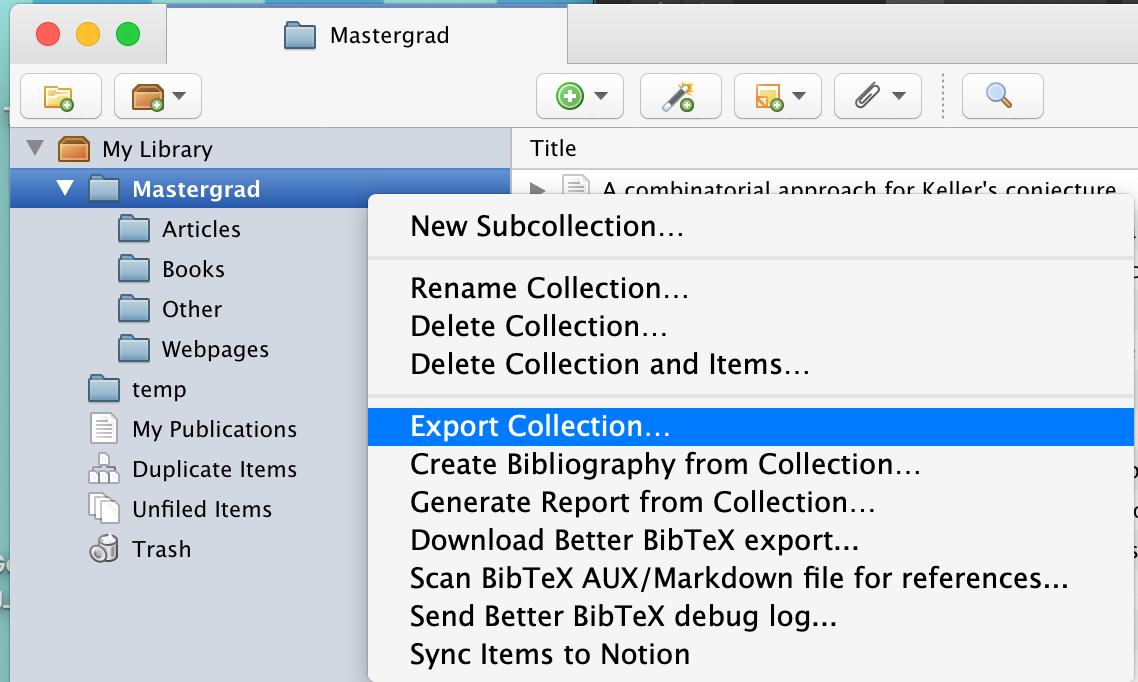
\includegraphics[width=0.9\linewidth]{x_zotero_1.png}
    \end{subfigure}\quad
    \begin{subfigure}{.33\textwidth}
        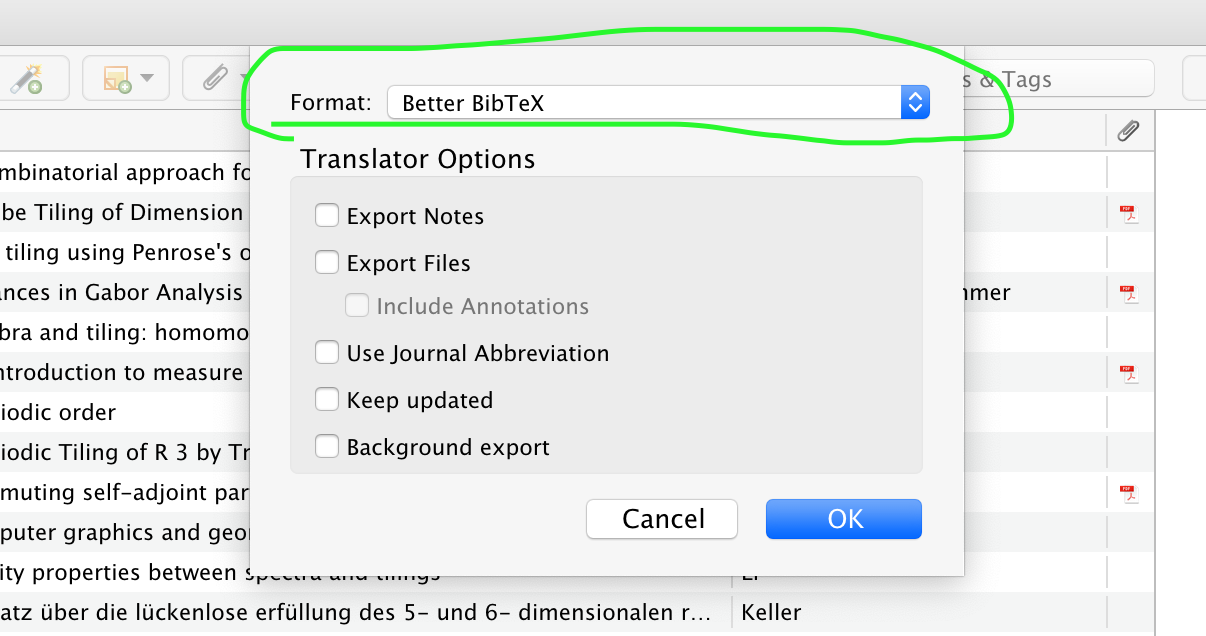
\includegraphics[width=0.9\linewidth]{x_zotero_2.png}
    \end{subfigure}\quad
    \begin{subfigure}{.33\textwidth}
        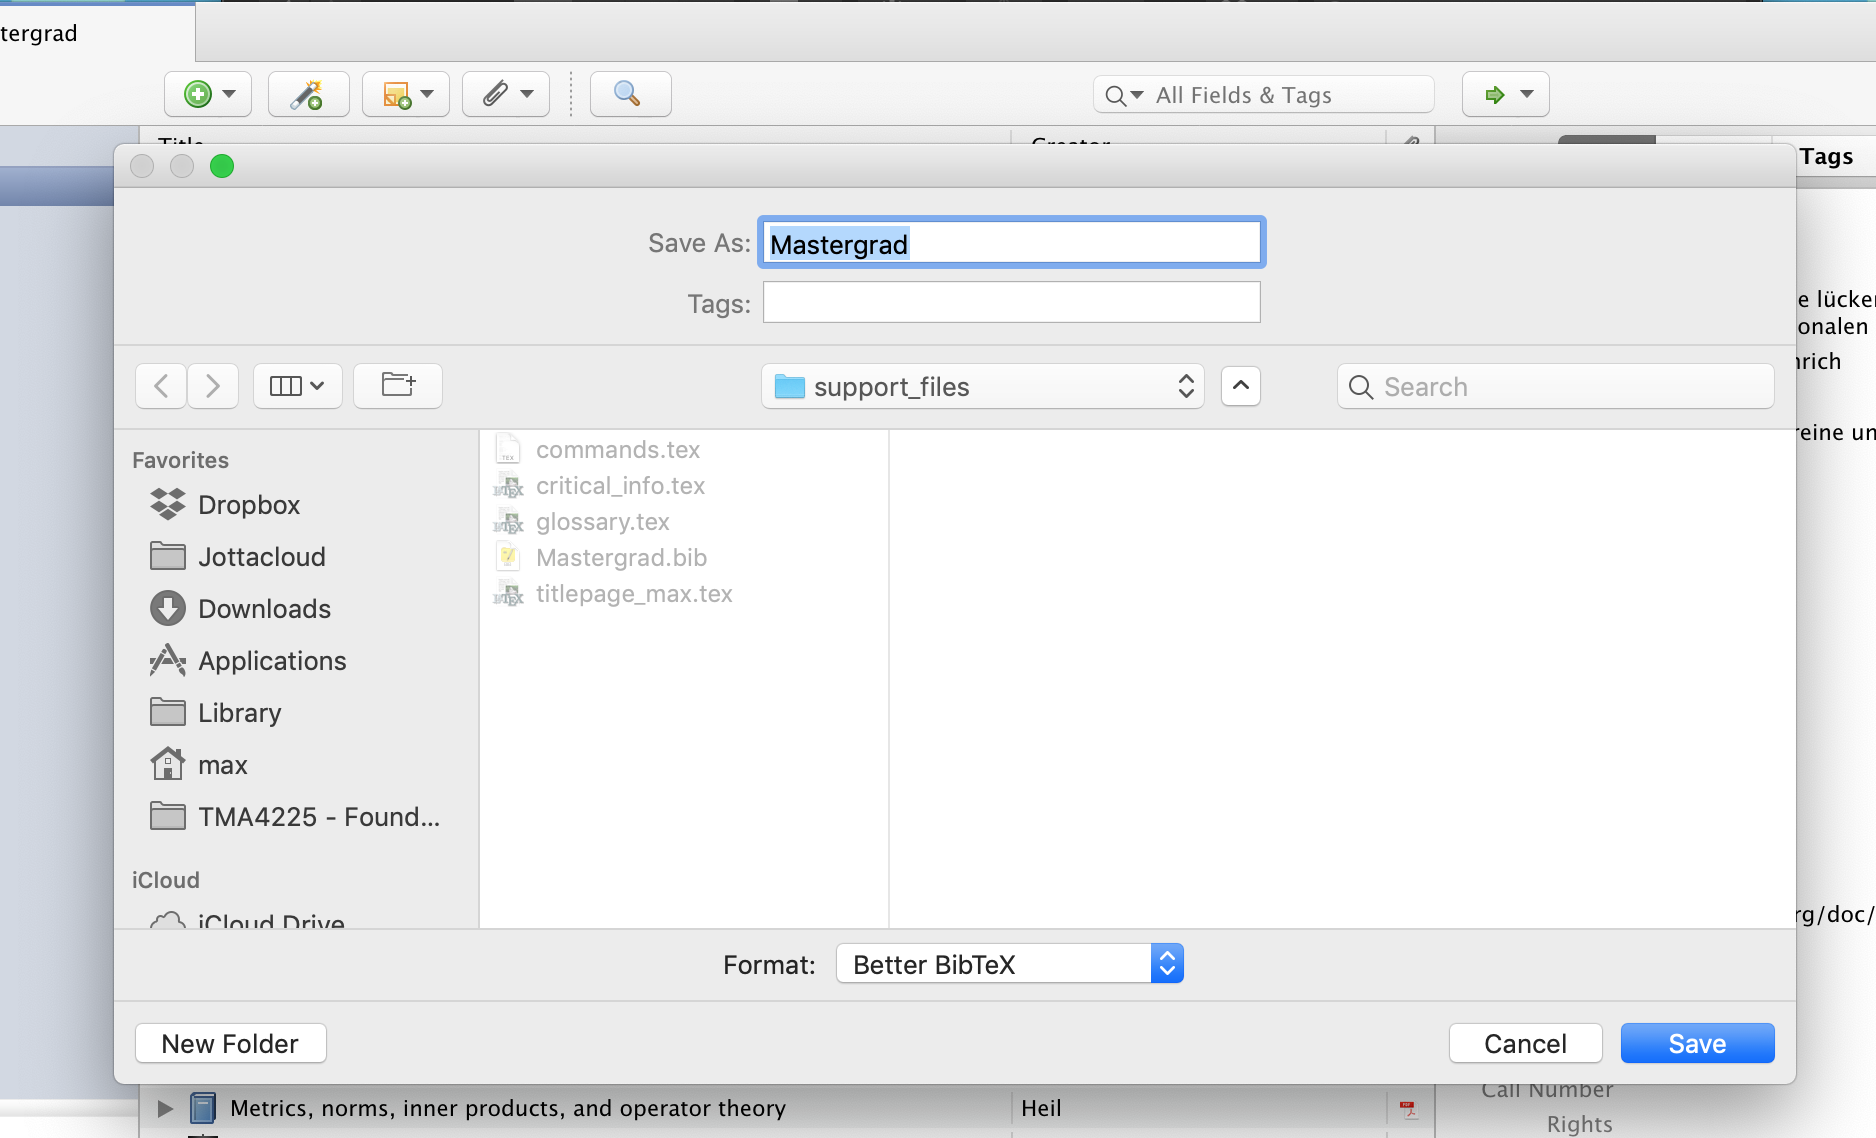
\includegraphics[width=0.9\linewidth]{x_zotero_3.png}
    \end{subfigure}
    \caption{Zotero export guide. Right-click and choose 'export collection'. Make sure the format is correct (BetterBibTeX). The first time you must manually navigate to the correct save spot, later on the Zotero should remember this.}
    \label{fig:zotero_figure}
\end{figure}


\textbf{Thesaurus}\\
Are you on a Mac? It has one of the best dictionaries and thesaurus for the English language — and it is built-in! Search for the program named "Dictionary" and choose your preferred languages in the app's preferences.  


\textbf{Write grammar free and correctly}\\
In addition to finding synonyms via the thesaurus above, chatgpt was used to find alternate words (also if needed, doublechecking its meaning via other sources). The author does not recommend chatgpt for writing content or solving problems it is much better (although not perfect) at rewriting your content, although sometimes the result is terrible. Also note, a paragraph might initially look good, but a read over a week later might result in you finding it made no sense at all. You will however rewrite parts of your thesis many times, and this is (usually) a \emph{good} thing <3
The most useful program for writing was Grammarly. chatgpt knows no grammar, and makes many many many grammar errors when writing. Grammarly is the bread and butter of spellchecking your thesis. An added benefit of Grammarly is that it can be integrated into many \LaTeX editors, including the one the author used (Vscode). If you need to buy it to get the extended functionality, it is well worth its steep price. 


\textbf{!Backup your document!}\\
If writing locally, plz make a backup!!! I kept two of my \LaTeX code; Paying a premium to Apple to back up my \emph{entire} desktop, documents, etc. to the cloud, and also synchronizing my one folder with the thesis itself to GitHub, a feature that is neatly integrated into Vscode, and easy to use.
GitHub, in addition to providing peace of mind, has a nice interface for viewing the history of all the changes to your document (that is only the changes you have pushed/saved to git, not the changes your editor itself keeps a history of (which is usually reset every time you close/open your document)). If you work with sensitive information or do not want your thesis public, the repository (name of the "folder" you have stored the theis) can be set to private.


\subsection{Tips on debugging \LaTeX}
\begin{itemize}
    \item Ask "chatgpt" with your problem/code/error message. This can often be helpful to understand WHAT has gone wrong. It may provide solutions that will not work. It might however be a good starting point for further search.
    \item Search the web
    \item Read the documentation for the package you are using on CTAN \url{https://www.ctan.org}
    \item Search the wiki (usually better than Wikipedia itself) \url{https://en.wikibooks.org/wiki/LaTeX}
    \item Ask a friend
\end{itemize}
If something is difficult to solve and is not directly related to the actual content of your thesis, consider making a note of what you have found out $+$ what do to next to try and solve it, and then move on to more pressing matters. 


\subsection{Tips for creating specific things in \LaTeX}
\textbf{For generating tables:}\\
\url{https://tablesgenerator.com}


\textbf{Genious for testing LaTeX code:}\\
\url{https://www.latex4technics.com}\\
Note that in the settings tab, one can change from compiling only equations to full \LaTeX. This can be useful for quickly testing figure code or other things in which you need a very very short compile time to test changes quickly. 
Important! If the page is refreshed, you lose all you have written. 


\textbf{Figures for biology, medicine, etc.}\\
\url{https://www.biorender.com}\\
Wish we had this for maths sometimes!


\textbf{Tikiz and some thoughts on drawings}\\
When creating drawings in \LaTeX, I would recommend doing so using the powerful internal package 'tikz'. It can sometimes be hard to use, but here is a few tips to get you started. First, a good source for some basic knowledge is \url{https://www.overleaf.com/learn/latex/TikZ_package}, or \url{https://tikz.dev} for more detailed information on specific parts of Tikiz and the different libraries one can use. The latter also provides some tutorials as well as providing a great overview of what it can be used to draw. The author also used chatgpt to generate some initial code, or to ask questions on "how to do this and that", but it cannot get you all the way. To test tikiz code the author used the webpage above 'latex4technics'. Functional, readable, and "good" figures are important. It is not recommended to do not push these "time thieves" to the final weeks. In addition to making your thesis better, it is also rewarding to complete a cool \LaTeX figure, and it was also the only thing my family partly understood of the thesis. A final mention is of this page which has tutorials for many types of figures and drawings \url{https://latexdraw.com}.

If one does not want to learn Tikiz, one can always play around with \href{https://www.mathcha.io/editor/vwPs1KFnvu2vIy2#}{matcha.io}, but it might not give you what you want, or the result is to simple of a drawing/figure. 


\subsection{Math specific pages}

\textbf{A simple and useful dictionary}\\
\url{https://matematikkradet.no/ordliste/}

\textbf{For drawing simple arrow diagrams}\\
\url{https://tikzcd.yichuanshen.de}

\textbf{The superior and more powerful diagram editor}\\
\url{https://q.uiver.app}

\textbf{Writing advice from Tao}\\
\url{https://terrytao.wordpress.com/advice-on-writing-papers/}



%* —————————————— NEW SECTION 
\section{Examples from my thesis}
Before and after for some figures
\begin{figure}[h!]%h!
    \centering
    \begin{subfigure}{.45\textwidth}
        \includegraphics[width=0.9\linewidth]{cper_dense_c.png}
    \end{subfigure}\quad
    \begin{subfigure}{.45\textwidth}
        %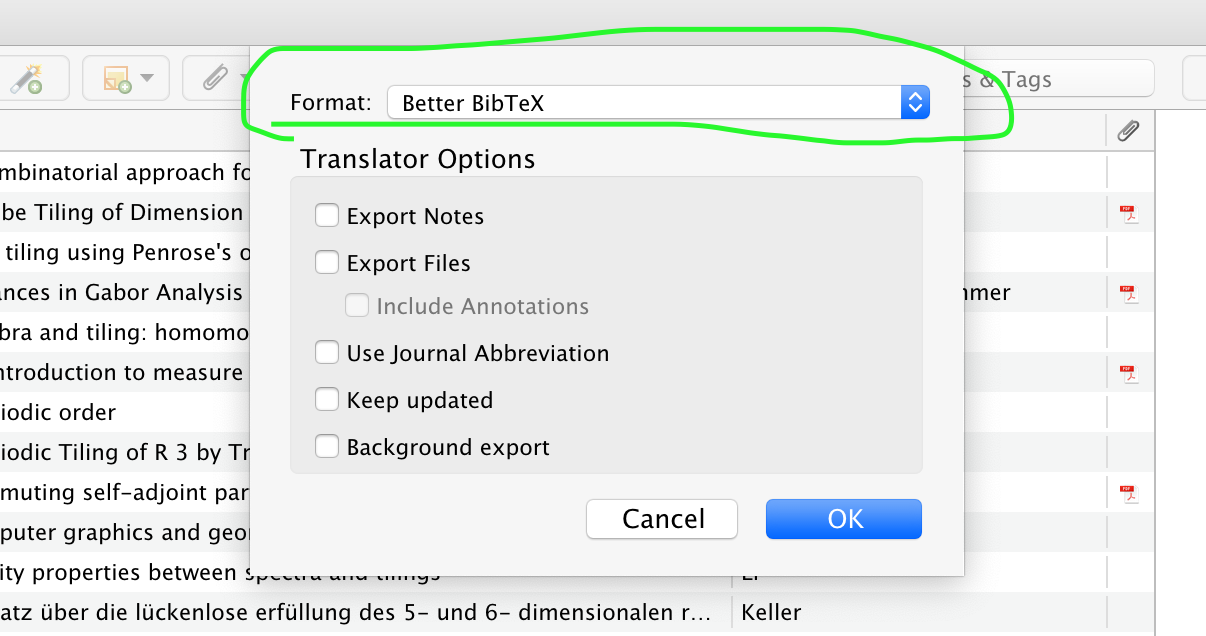
\includegraphics[width=0.9\linewidth]{x_zotero_2.png}
        

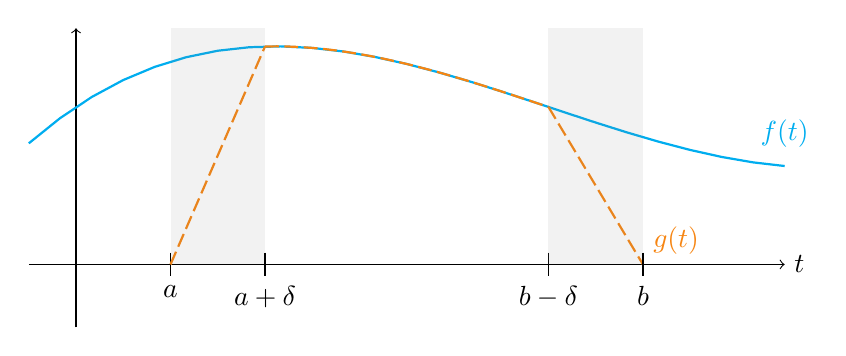
\begin{tikzpicture}[xscale=6,yscale=2]
    %* Draw axes
    \draw[->] (-0.1,0) -- (1.5,0) node[right] {$t$};  % går fra -0.3 til 1.5 på X aksen
    \draw[->] (0,-0.4) -- (0,1.5); %node[above] {$y$};  % går fra -0.4 til 1.5 på Y aksen
    
    %* Plot polynomial function
    \draw[cyan, thick, domain = -0.1:1.5] plot (\x, {(\x-1)^3 - (\x-1) + 1}) node[above, yshift=1mm] {$f(t)$};


    %* Draw labeled marks on the x-axis
    \foreach \x in { 0.2 }{
        \draw (\x,0.075) -- (\x,-0.075) node[below] {$a$}; % Lengden på linjen først
        %\draw[dashed] (\x,0) -- (\x,1.5);
        \draw[BurntOrange, dash pattern={on 5pt off 2pt}, thick] (\x,0) -- (0.4,{(0.4-1)^3 - (0.4-1) + 1});  % end value is the function value
    }

    %* Shade area between the points above and below
    \fill[gray, opacity=0.1] (0.2,0) -- (0.2,1.5) -- (0.4,1.5) -- (0.4,0) -- cycle;
    %\draw[pattern={north east lines},pattern color=gray] (0.2,0) rectangle +(0.2,1.5);

    %* Draw labeled marks on the x-axis
    \foreach \x in { 0.4 }{
        \draw (\x,0.075) -- (\x,-0.075) node[below] {$a+\delta$}; % Lengden på linjen først
        %\draw[dashed] (\x,0) -- (\x,1.5);
    }

    %* draw the middle parts of the approximating function g  —————— MIDDLE ——————
    %\draw[red, thick, dashed, domain=0.4:1] plot (\x, {(\x-1)^3 - (\x-1) + 1}) node[anchor=south east, yshift=2mm] {$g(t)$};
    %\draw[BurntOrange, thick, dashed, domain=0.4:1] plot (\x, {(\x-1)^3 - (\x-1) + 1});
    \draw[BurntOrange, thick, dash pattern={on 5pt off 2pt}, domain=0.4:1] plot (\x, {(\x-1)^3 - (\x-1) + 1});
    

    %* Draw labeled marks on the x-axis
    \foreach \x in { 1 }{
        \draw (\x,0.075) -- (\x,-0.075) node[below] {$b-\delta$}; % Lengden på linjen først
        %\draw[dashed] (\x,0) -- (\x,1.5);
        \draw[BurntOrange, dash pattern={on 5pt off 2pt}, thick] (\x,{(\x-1)^3 - (\x-1) + 1}) -- (1.2,0) node[anchor=south west, yshift=0mm] {$g(t)$};  % end value is the function value
    }

    %* Shade area between the points above and below
    \fill[gray, opacity=0.1] (1,0) -- (1,1.5) -- (1.2,1.5) -- (1.2,0) -- cycle;

    %* Draw labeled marks on the x-axis
    \foreach \x in { 1.2 }{
        \draw (\x,0.075) -- (\x,-0.075) node[below] {$b$};
        %\draw[dashed] (\x,0) -- (\x,1.5);
    }

    %\fill[gray, opacity=0.3] (0.2,0) -- (0.2,{(0.2-1)^3 - (0.2-1) + 1}) -- (0.4,{(0.4-1)^3 - (0.4-1) + 1}) -- (0.4,0) -- cycle;

\end{tikzpicture}


\mycomment{  %! Whole middle fill with dotted lines
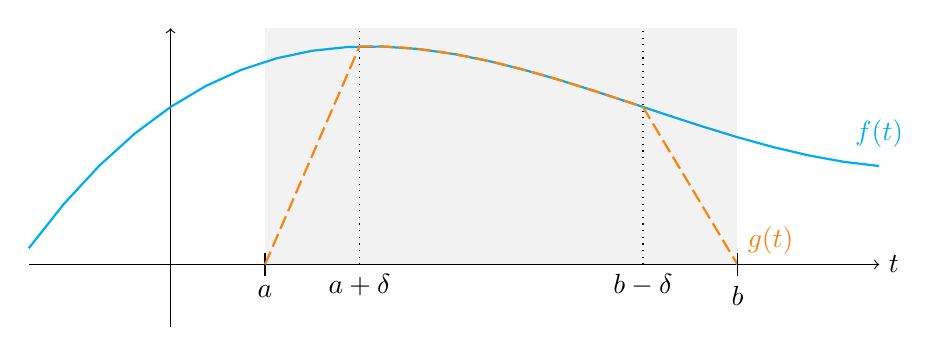
\begin{tikzpicture}[xscale=6,yscale=2]
    %* Draw axes
    \draw[->] (-0.3,0) -- (1.5,0) node[right] {$t$};  % går fra -0.3 til 1.5 på X aksen
    \draw[->] (0,-0.4) -- (0,1.5); %node[above] {$y$};  % går fra -0.4 til 1.5 på Y aksen
    
    %* Plot polynomial function
    \draw[cyan, thick, domain=-0.3:1.5] plot (\x, {(\x-1)^3 - (\x-1) + 1}) node[above, yshift=1mm] {$f(t)$};
    %* Shade area 
    \fill[gray, opacity=0.1] (0.2,0) -- (0.2,1.5) -- (1.2,1.5) -- (1.2,0) -- cycle;

    %* Draw labeled marks on the x-axis
    \foreach \x in { 0.2 }{
        \draw (\x,0.075) -- (\x,-0.075) node[below] {$a$}; % Lengden på linjen først
        %\draw[dashed] (\x,0) -- (\x,1.5);
        \draw[BurntOrange, dash pattern={on 5pt off 2pt}, thick] (\x,0) -- (0.4,{(0.4-1)^3 - (0.4-1) + 1});  % end value is the function value
    }

    %* Draw labeled marks on the x-axis
    \foreach \x in { 0.4 }{
        \draw (\x,0) -- (\x,-0.001) node[below] {$a+\delta$}; % Lengden på linjen først
        \draw[dotted] (\x,0) -- (\x,1.5);
    }

    %* draw the middle parts of the approximating function g  —————— MIDDLE ——————
    %\draw[red, thick, dashed, domain=0.4:1] plot (\x, {(\x-1)^3 - (\x-1) + 1}) node[anchor=south east, yshift=2mm] {$g(t)$};
    %\draw[BurntOrange, thick, dashed, domain=0.4:1] plot (\x, {(\x-1)^3 - (\x-1) + 1});
    \draw[BurntOrange, thick, dash pattern={on 5pt off 2pt}, domain=0.4:1] plot (\x, {(\x-1)^3 - (\x-1) + 1});
    

    %* Draw labeled marks on the x-axis
    \foreach \x in { 1 }{
        \draw (\x,0) -- (\x,-0.001) node[below] {$b-\delta$}; % Lengden på linjen først
        \draw[dotted] (\x,0) -- (\x,1.5);
        \draw[BurntOrange, dash pattern={on 5pt off 2pt}, thick] (\x,{(\x-1)^3 - (\x-1) + 1}) -- (1.2,0) node[anchor=south west, yshift=0mm] {$g(t)$};  % end value is the function value
    }


    %* Draw labeled marks on the x-axis
    \foreach \x in { 1.2 }{
        \draw (\x,0.075) -- (\x,-0.075) node[below] {$b$};
        %\draw[dashed] (\x,0) -- (\x,1.5);
    }

    %\fill[gray, opacity=0.3] (0.2,0) -- (0.2,{(0.2-1)^3 - (0.2-1) + 1}) -- (0.4,{(0.4-1)^3 - (0.4-1) + 1}) -- (0.4,0) -- cycle;

\end{tikzpicture}
}

\mycomment{  %! Whole middle fill with dashed lines
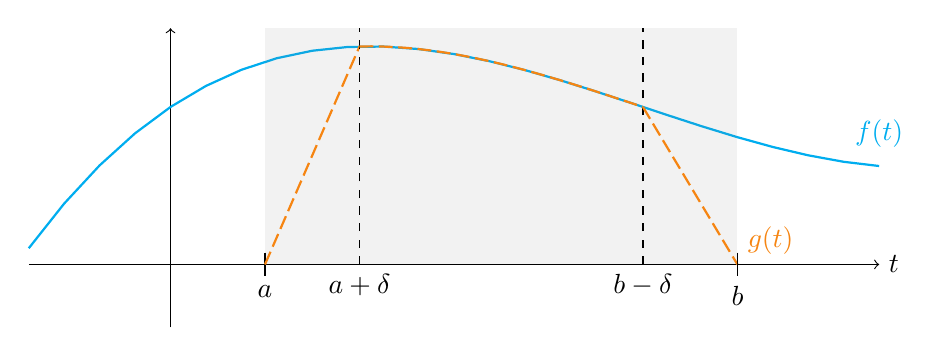
\begin{tikzpicture}[xscale=6,yscale=2]
    %* Draw axes
    \draw[->] (-0.3,0) -- (1.5,0) node[right] {$t$};  % går fra -0.3 til 1.5 på X aksen
    \draw[->] (0,-0.4) -- (0,1.5); %node[above] {$y$};  % går fra -0.4 til 1.5 på Y aksen
    
    %* Plot polynomial function
    \draw[cyan, thick, domain=-0.3:1.5] plot (\x, {(\x-1)^3 - (\x-1) + 1}) node[above, yshift=1mm] {$f(t)$};
    %* Shade area 
    \fill[gray, opacity=0.1] (0.2,0) -- (0.2,1.5) -- (1.2,1.5) -- (1.2,0) -- cycle;

    %* Draw labeled marks on the x-axis
    \foreach \x in { 0.2 }{
        \draw (\x,0.075) -- (\x,-0.075) node[below] {$a$}; % Lengden på linjen først
        %\draw[dashed] (\x,0) -- (\x,1.5);
        \draw[BurntOrange, dash pattern={on 5pt off 2pt}, thick] (\x,0) -- (0.4,{(0.4-1)^3 - (0.4-1) + 1});  % end value is the function value
    }

    %* Draw labeled marks on the x-axis
    \foreach \x in { 0.4 }{
        \draw (\x,0) -- (\x,-0.001) node[below] {$a+\delta$}; % Lengden på linjen først
        \draw[dashed] (\x,0) -- (\x,1.5);
    }

    %* draw the middle parts of the approximating function g  —————— MIDDLE ——————
    %\draw[red, thick, dashed, domain=0.4:1] plot (\x, {(\x-1)^3 - (\x-1) + 1}) node[anchor=south east, yshift=2mm] {$g(t)$};
    %\draw[BurntOrange, thick, dashed, domain=0.4:1] plot (\x, {(\x-1)^3 - (\x-1) + 1});
    \draw[BurntOrange, thick, dash pattern={on 5pt off 2pt}, domain=0.4:1] plot (\x, {(\x-1)^3 - (\x-1) + 1});
    

    %* Draw labeled marks on the x-axis
    \foreach \x in { 1 }{
        \draw (\x,0) -- (\x,-0.001) node[below] {$b-\delta$}; % Lengden på linjen først
        \draw[dashed] (\x,0) -- (\x,1.5);
        \draw[BurntOrange, dash pattern={on 5pt off 2pt}, thick] (\x,{(\x-1)^3 - (\x-1) + 1}) -- (1.2,0) node[anchor=south west, yshift=0mm] {$g(t)$};  % end value is the function value
    }


    %* Draw labeled marks on the x-axis
    \foreach \x in { 1.2 }{
        \draw (\x,0.075) -- (\x,-0.075) node[below] {$b$};
        %\draw[dashed] (\x,0) -- (\x,1.5);
    }

    %\fill[gray, opacity=0.3] (0.2,0) -- (0.2,{(0.2-1)^3 - (0.2-1) + 1}) -- (0.4,{(0.4-1)^3 - (0.4-1) + 1}) -- (0.4,0) -- cycle;

\end{tikzpicture}
}


\mycomment{  %! Whole middle fill with dashed lines and solid lines at the end
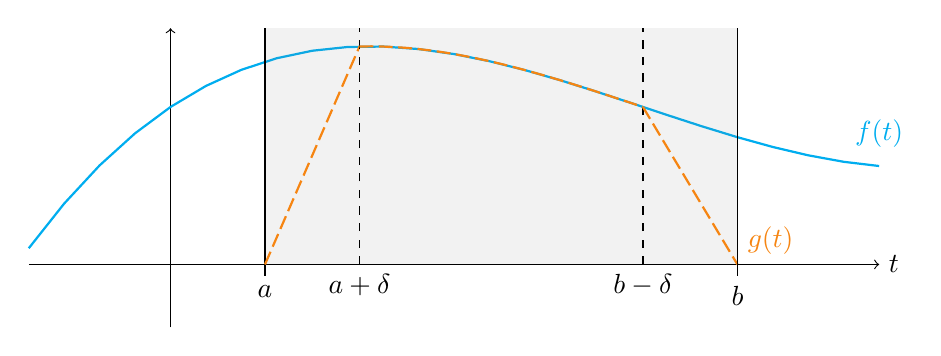
\begin{tikzpicture}[xscale=6,yscale=2]
    %* Draw axes
    \draw[->] (-0.3,0) -- (1.5,0) node[right] {$t$};  % går fra -0.3 til 1.5 på X aksen
    \draw[->] (0,-0.4) -- (0,1.5); %node[above] {$y$};  % går fra -0.4 til 1.5 på Y aksen
    
    %* Plot polynomial function
    \draw[cyan, thick, domain=-0.3:1.5] plot (\x, {(\x-1)^3 - (\x-1) + 1}) node[above, yshift=1mm] {$f(t)$};
    %* Shade area 
    \fill[gray, opacity=0.1] (0.2,0) -- (0.2,1.5) -- (1.2,1.5) -- (1.2,0) -- cycle;

    %* Draw labeled marks on the x-axis
    \foreach \x in { 0.2 }{
        \draw (\x,0.075) -- (\x,-0.075) node[below] {$a$}; % Lengden på linjen først
        \draw(\x,0) -- (\x,1.5);
        \draw[BurntOrange, dash pattern={on 5pt off 2pt}, thick] (\x,0) -- (0.4,{(0.4-1)^3 - (0.4-1) + 1});  % end value is the function value
    }

    %* Draw labeled marks on the x-axis
    \foreach \x in { 0.4 }{
        \draw (\x,0) -- (\x,-0.001) node[below] {$a+\delta$}; % Lengden på linjen først
        \draw [dashed] (\x,0) -- (\x,1.5);
    }

    %* draw the middle parts of the approximating function g  —————— MIDDLE ——————
    %\draw[red, thick, dashed, domain=0.4:1] plot (\x, {(\x-1)^3 - (\x-1) + 1}) node[anchor=south east, yshift=2mm] {$g(t)$};
    %\draw[BurntOrange, thick, dashed, domain=0.4:1] plot (\x, {(\x-1)^3 - (\x-1) + 1});
    \draw[BurntOrange, thick, dash pattern={on 5pt off 2pt}, domain=0.4:1] plot (\x, {(\x-1)^3 - (\x-1) + 1});
    

    %* Draw labeled marks on the x-axis
    \foreach \x in { 1 }{
        \draw (\x,0) -- (\x,-0.001) node[below] {$b-\delta$}; % Lengden på linjen først
        \draw [dashed] (\x,0) -- (\x,1.5);
        \draw[BurntOrange, dash pattern={on 5pt off 2pt}, thick] (\x,{(\x-1)^3 - (\x-1) + 1}) -- (1.2,0) node[anchor=south west, yshift=0mm] {$g(t)$};  % end value is the function value
    }


    %* Draw labeled marks on the x-axis
    \foreach \x in { 1.2 }{
        \draw (\x,0.075) -- (\x,-0.075) node[below] {$b$};
        \draw (\x,0) -- (\x,1.5);
    }

    %\fill[gray, opacity=0.3] (0.2,0) -- (0.2,{(0.2-1)^3 - (0.2-1) + 1}) -- (0.4,{(0.4-1)^3 - (0.4-1) + 1}) -- (0.4,0) -- cycle;

\end{tikzpicture}
}
    \end{subfigure}
\end{figure}


\begin{figure}[h!]%h!
    \centering
    \begin{subfigure}{.45\textwidth}
        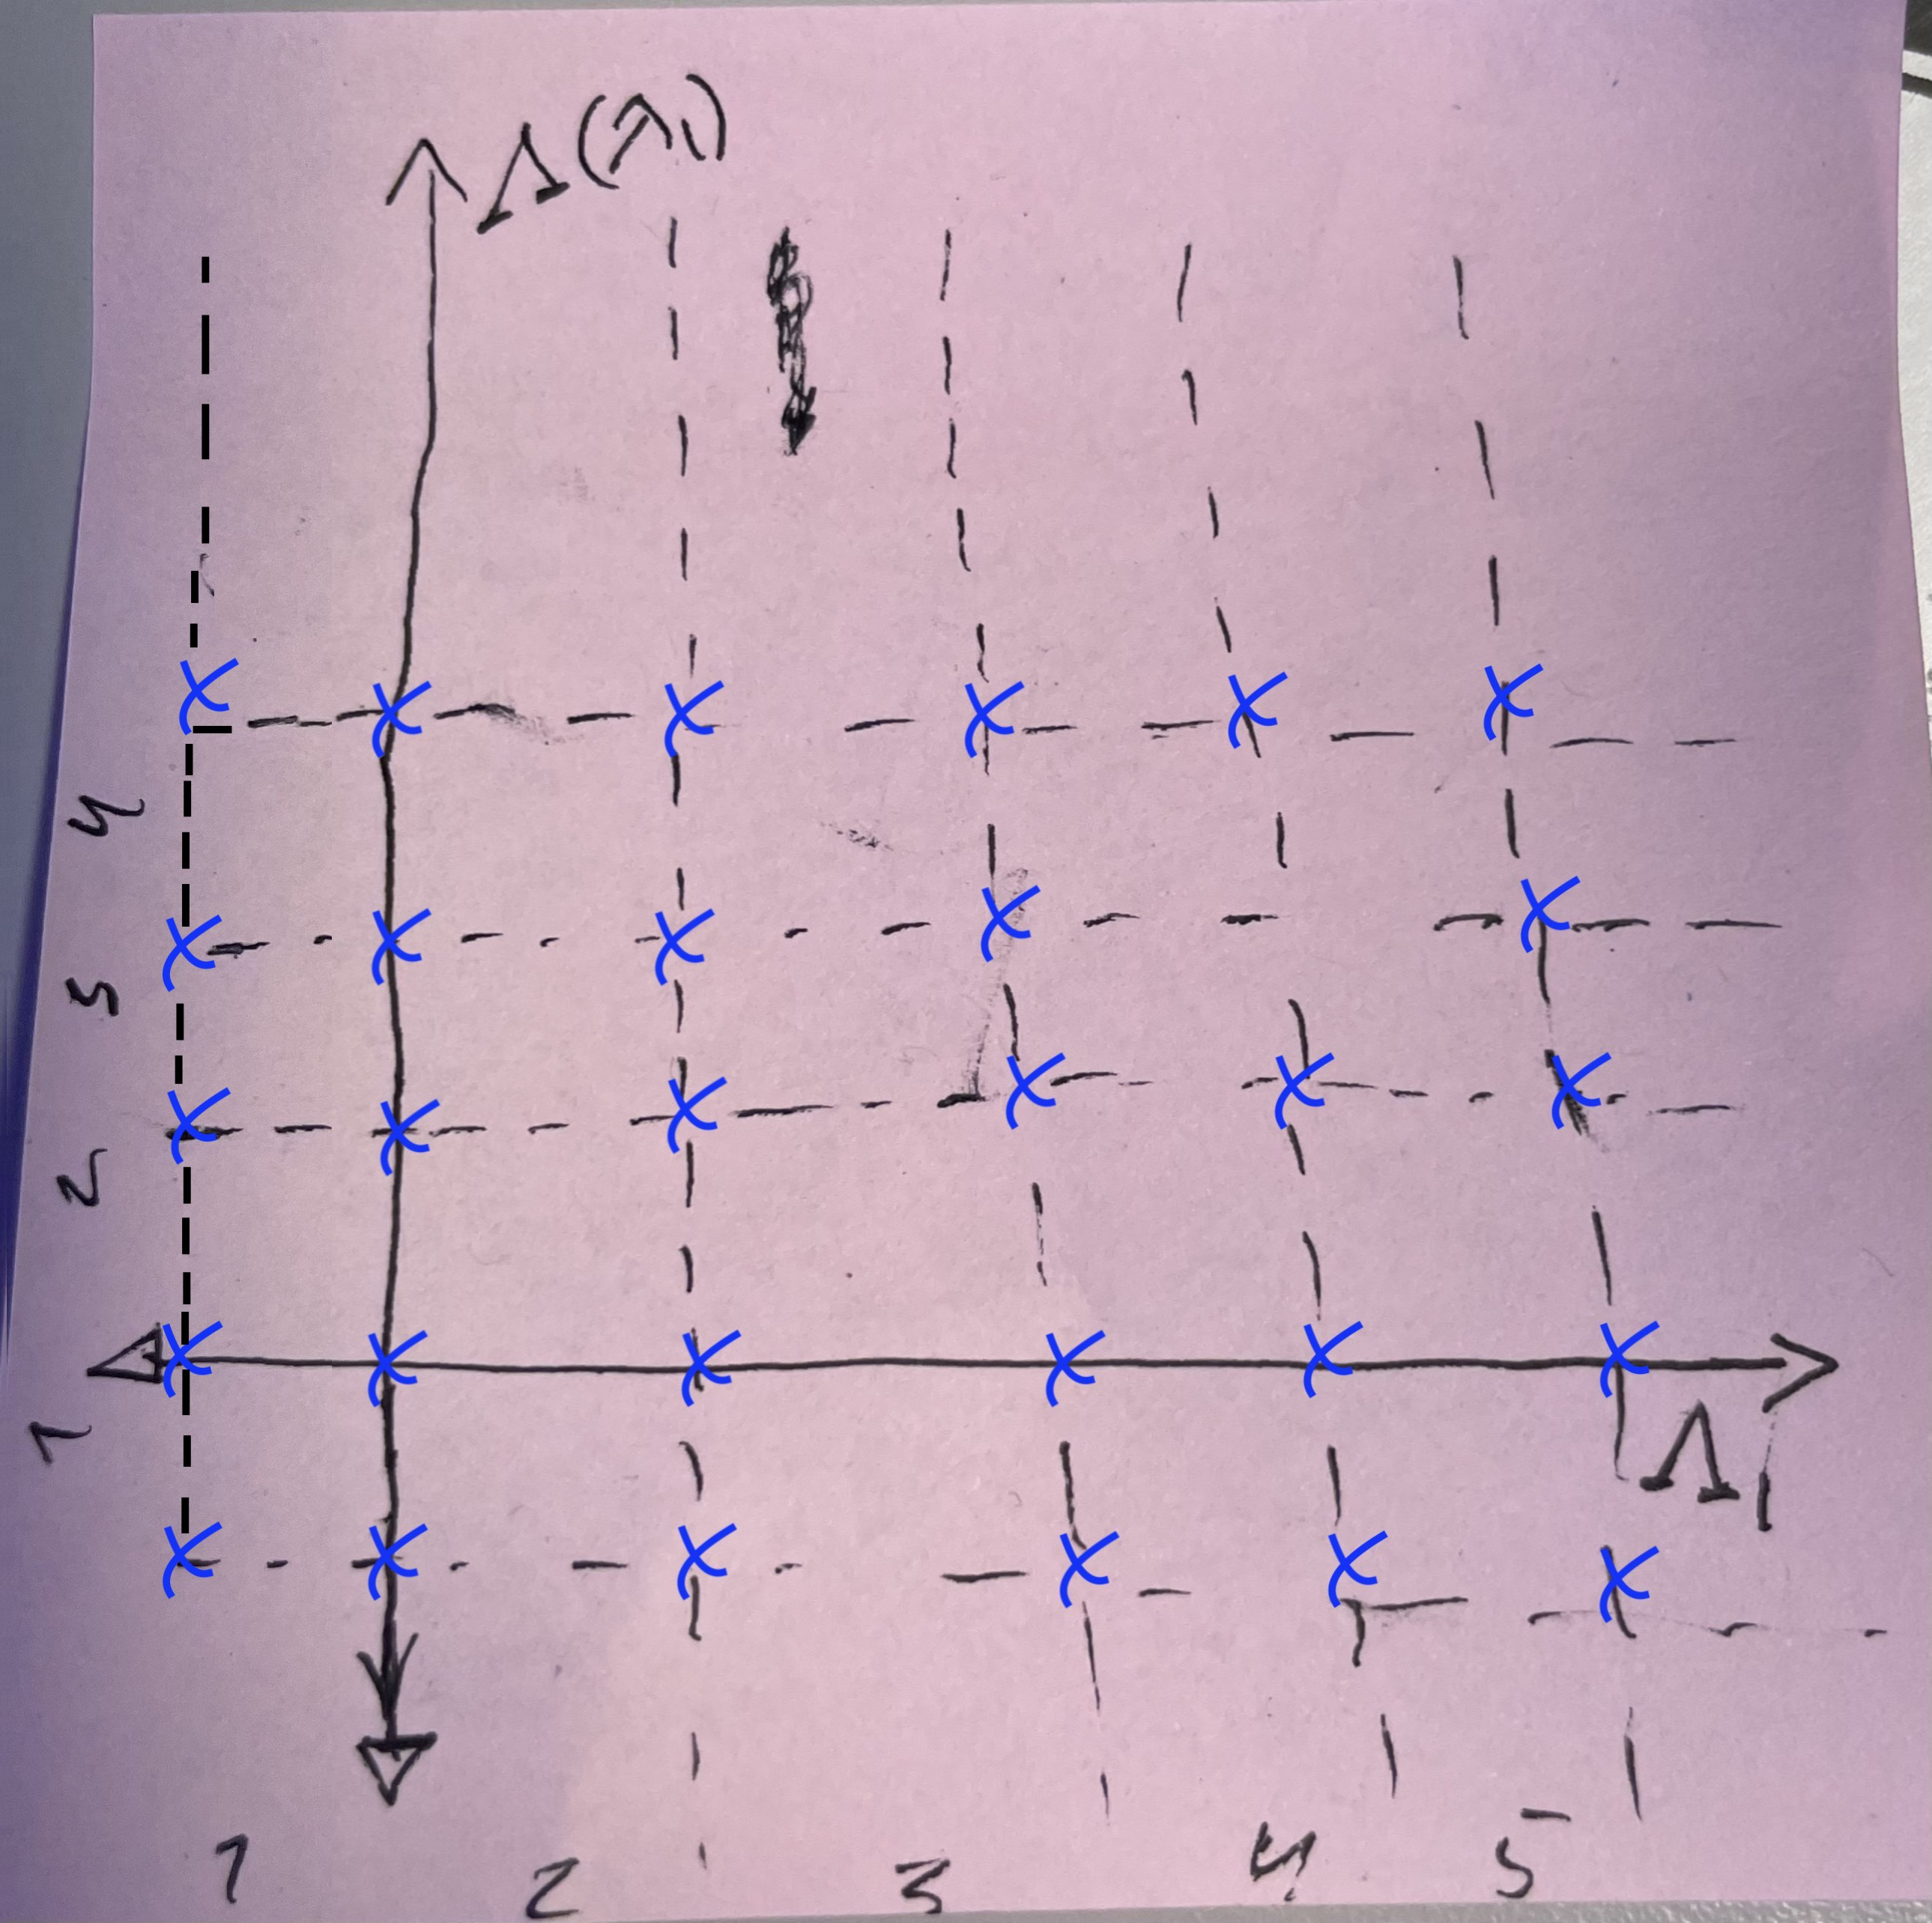
\includegraphics[width=0.9\linewidth]{spec_no_shift.jpg}
    \end{subfigure}\quad
    \begin{subfigure}{.45\textwidth}
        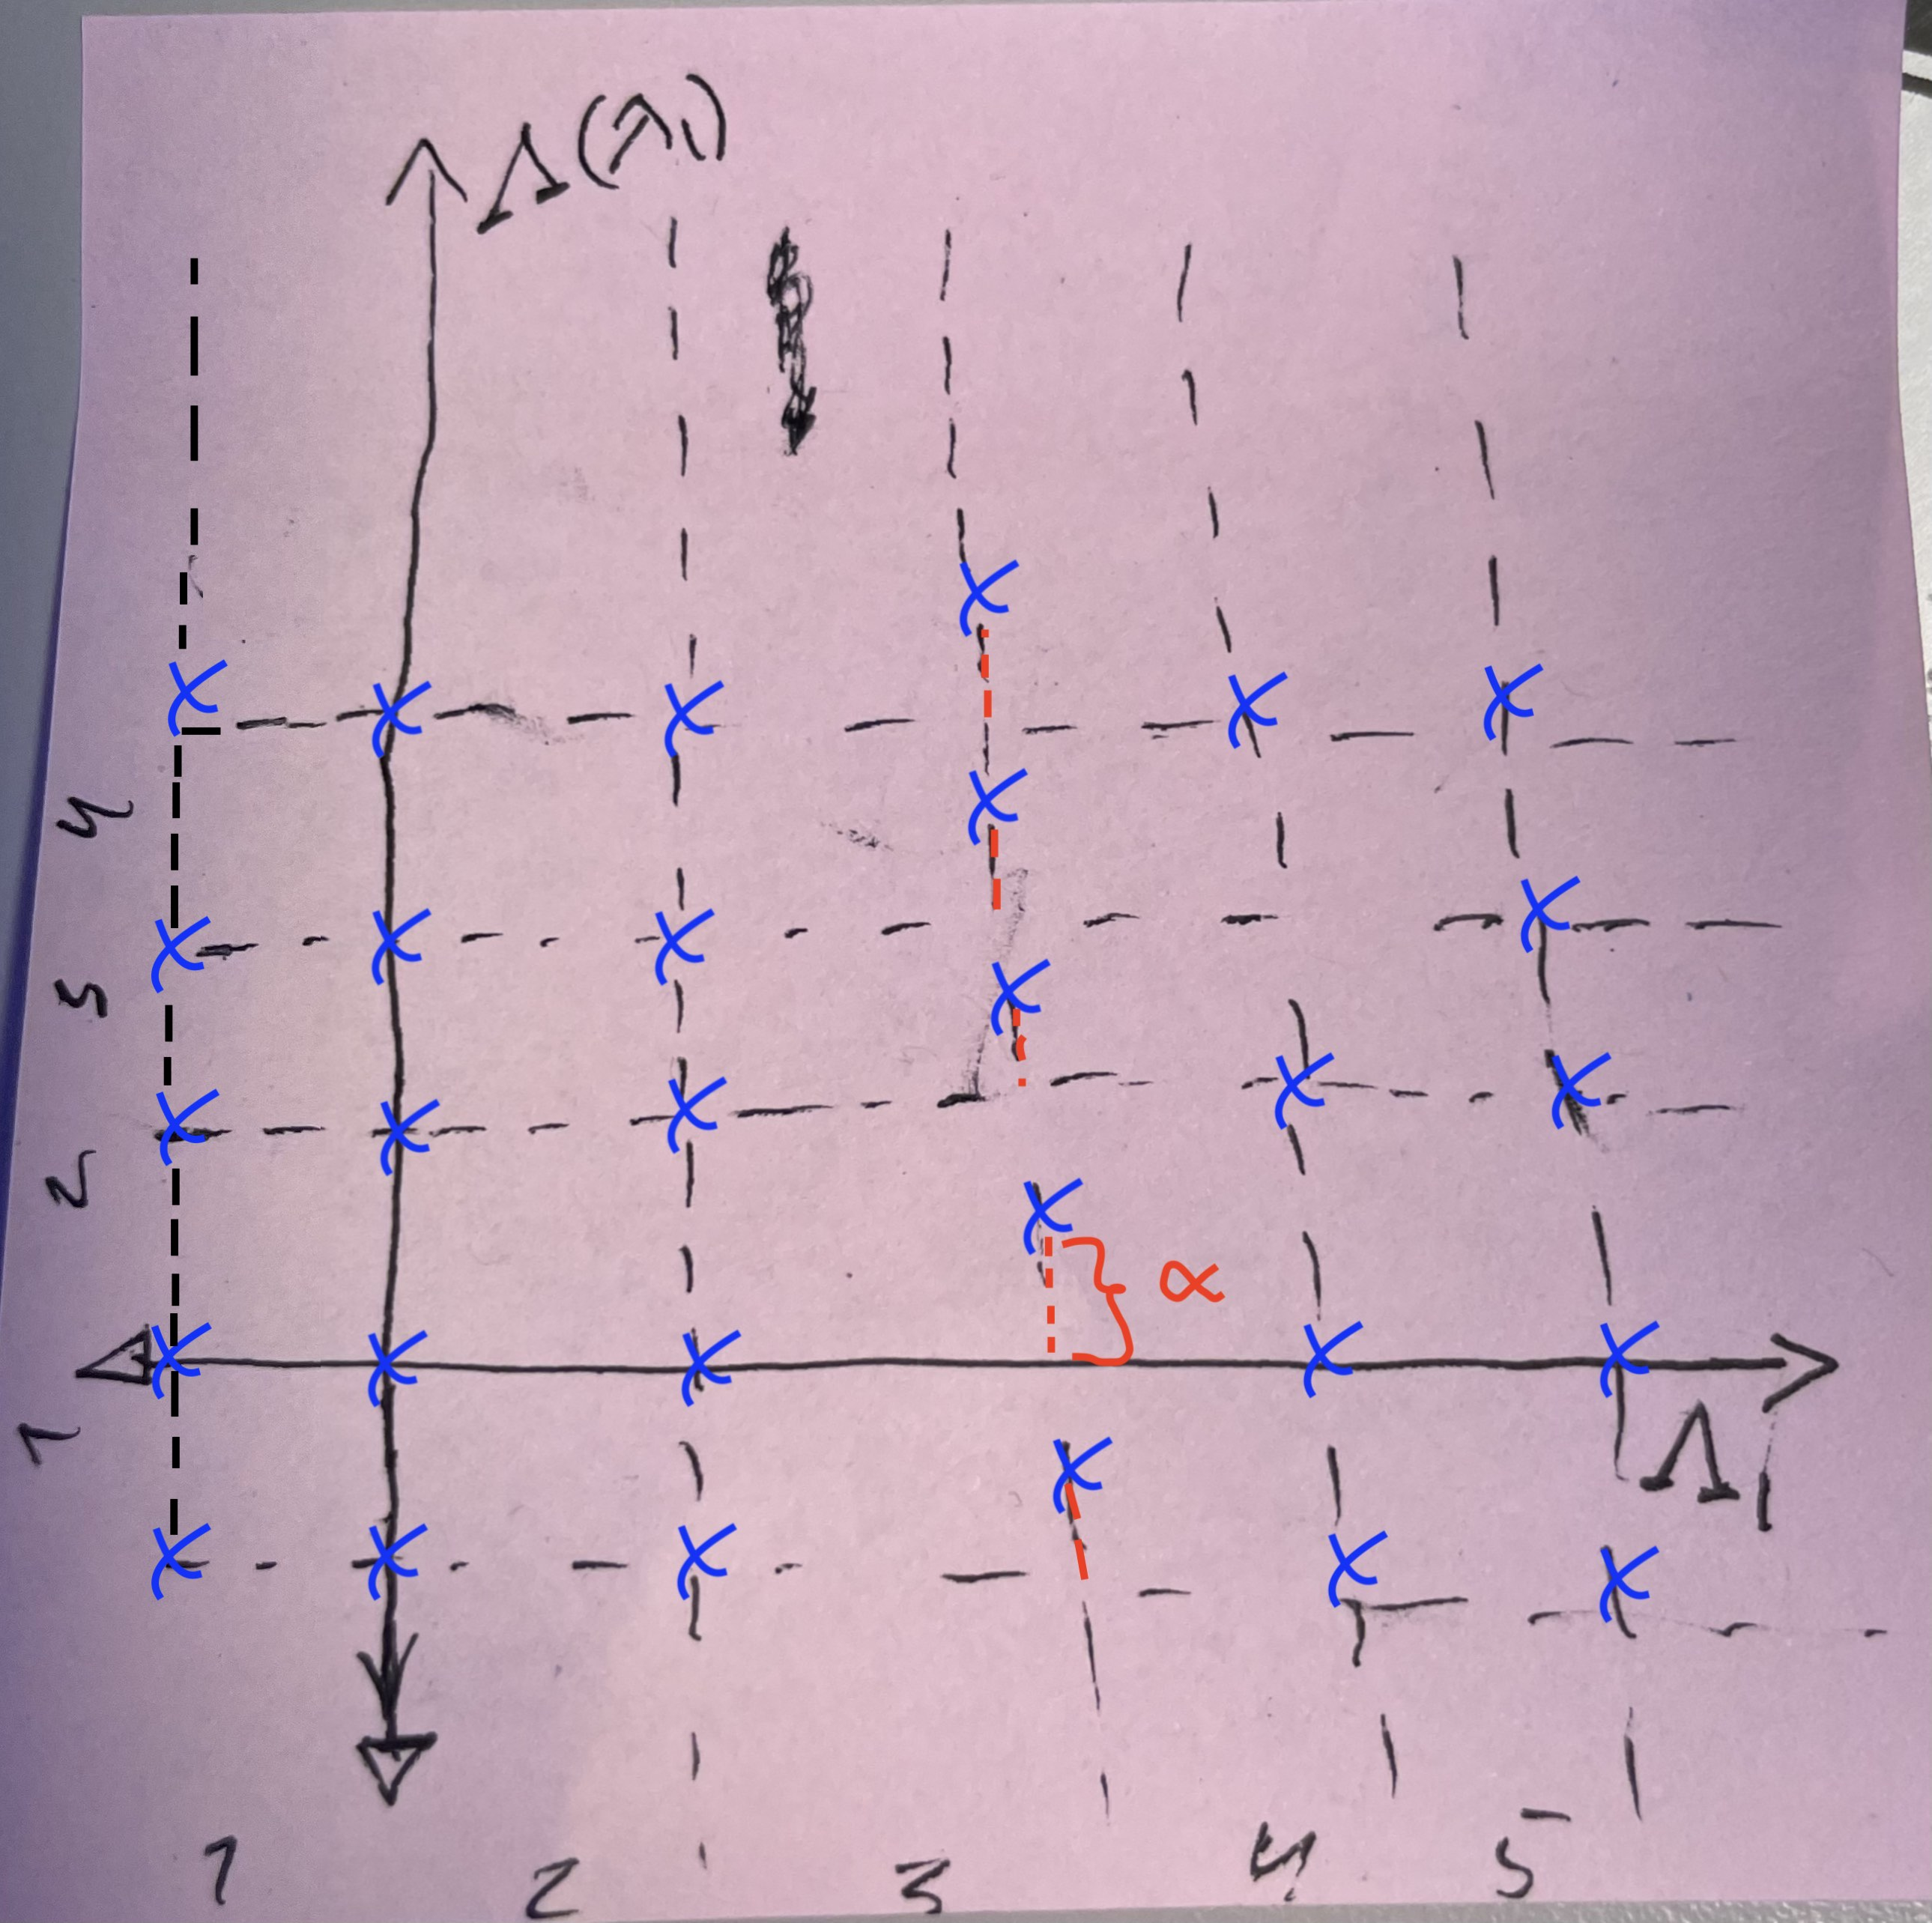
\includegraphics[width=0.9\linewidth]{spec_single_shift.jpg}
    \end{subfigure}\\
    \begin{subfigure}{.45\textwidth}
        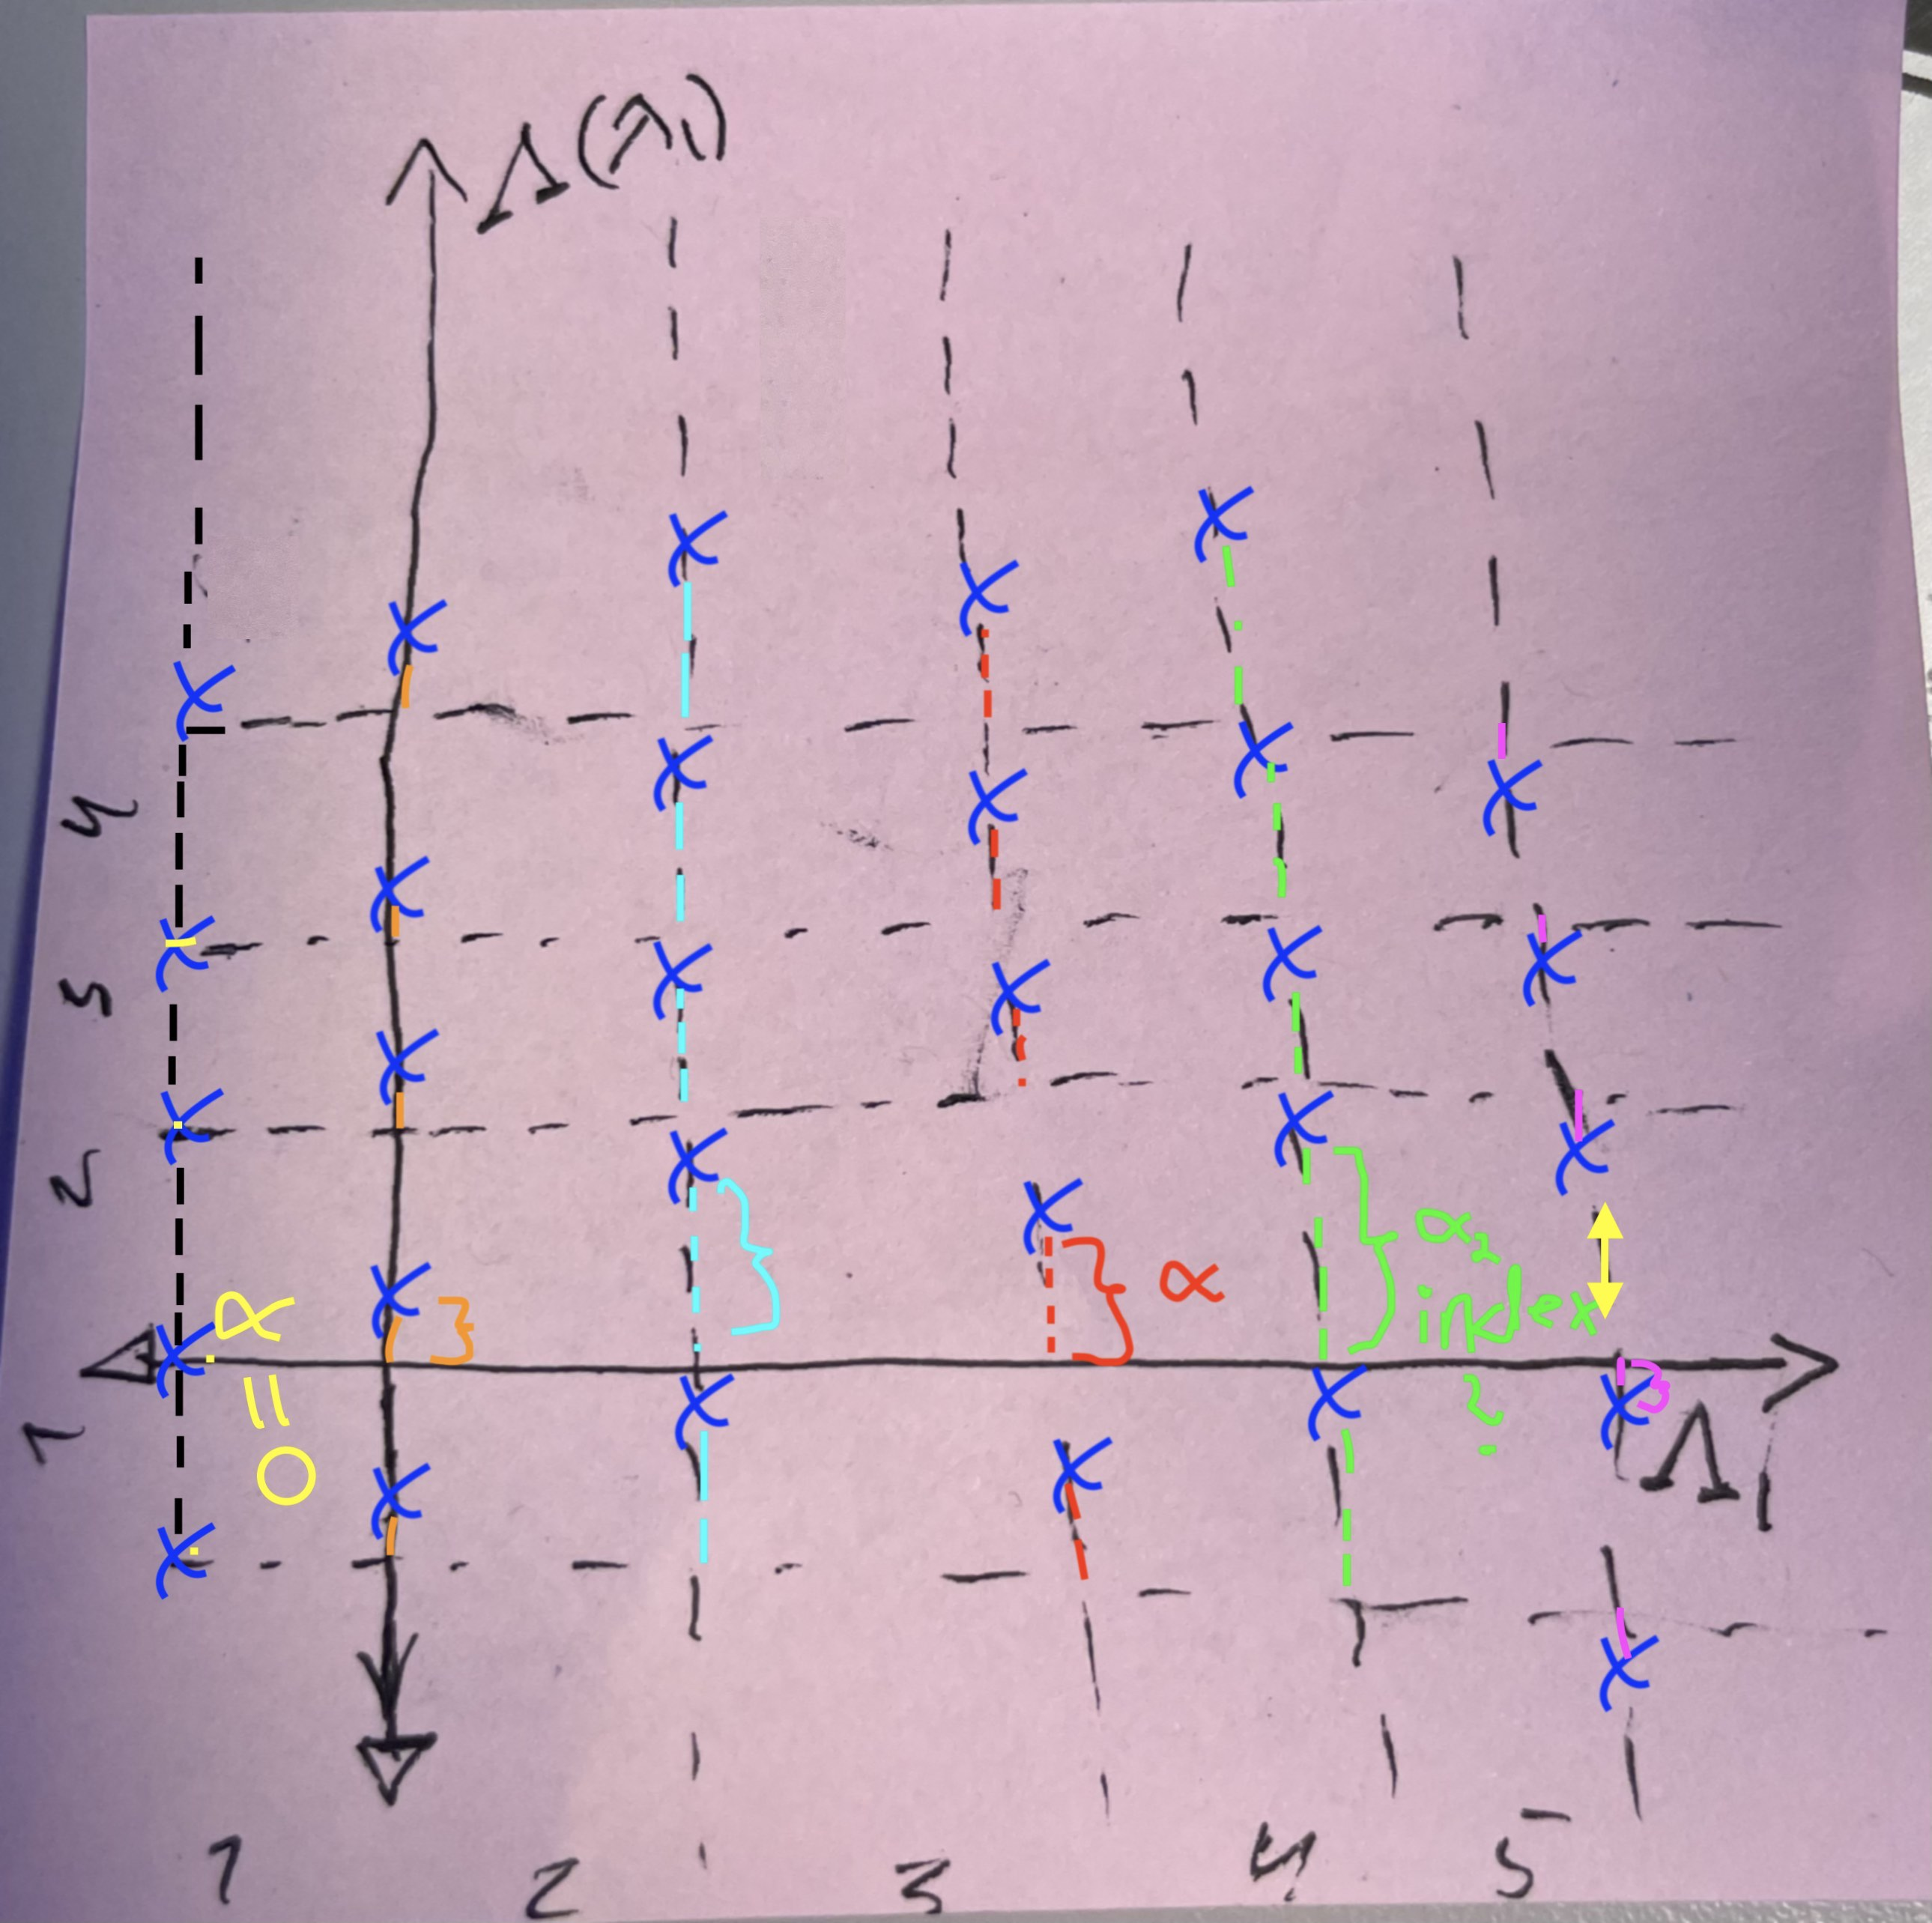
\includegraphics[width=0.9\linewidth]{multiple_shift_left_zero.jpg}
    \end{subfigure}\quad
    \begin{subfigure}{.45\textwidth}
        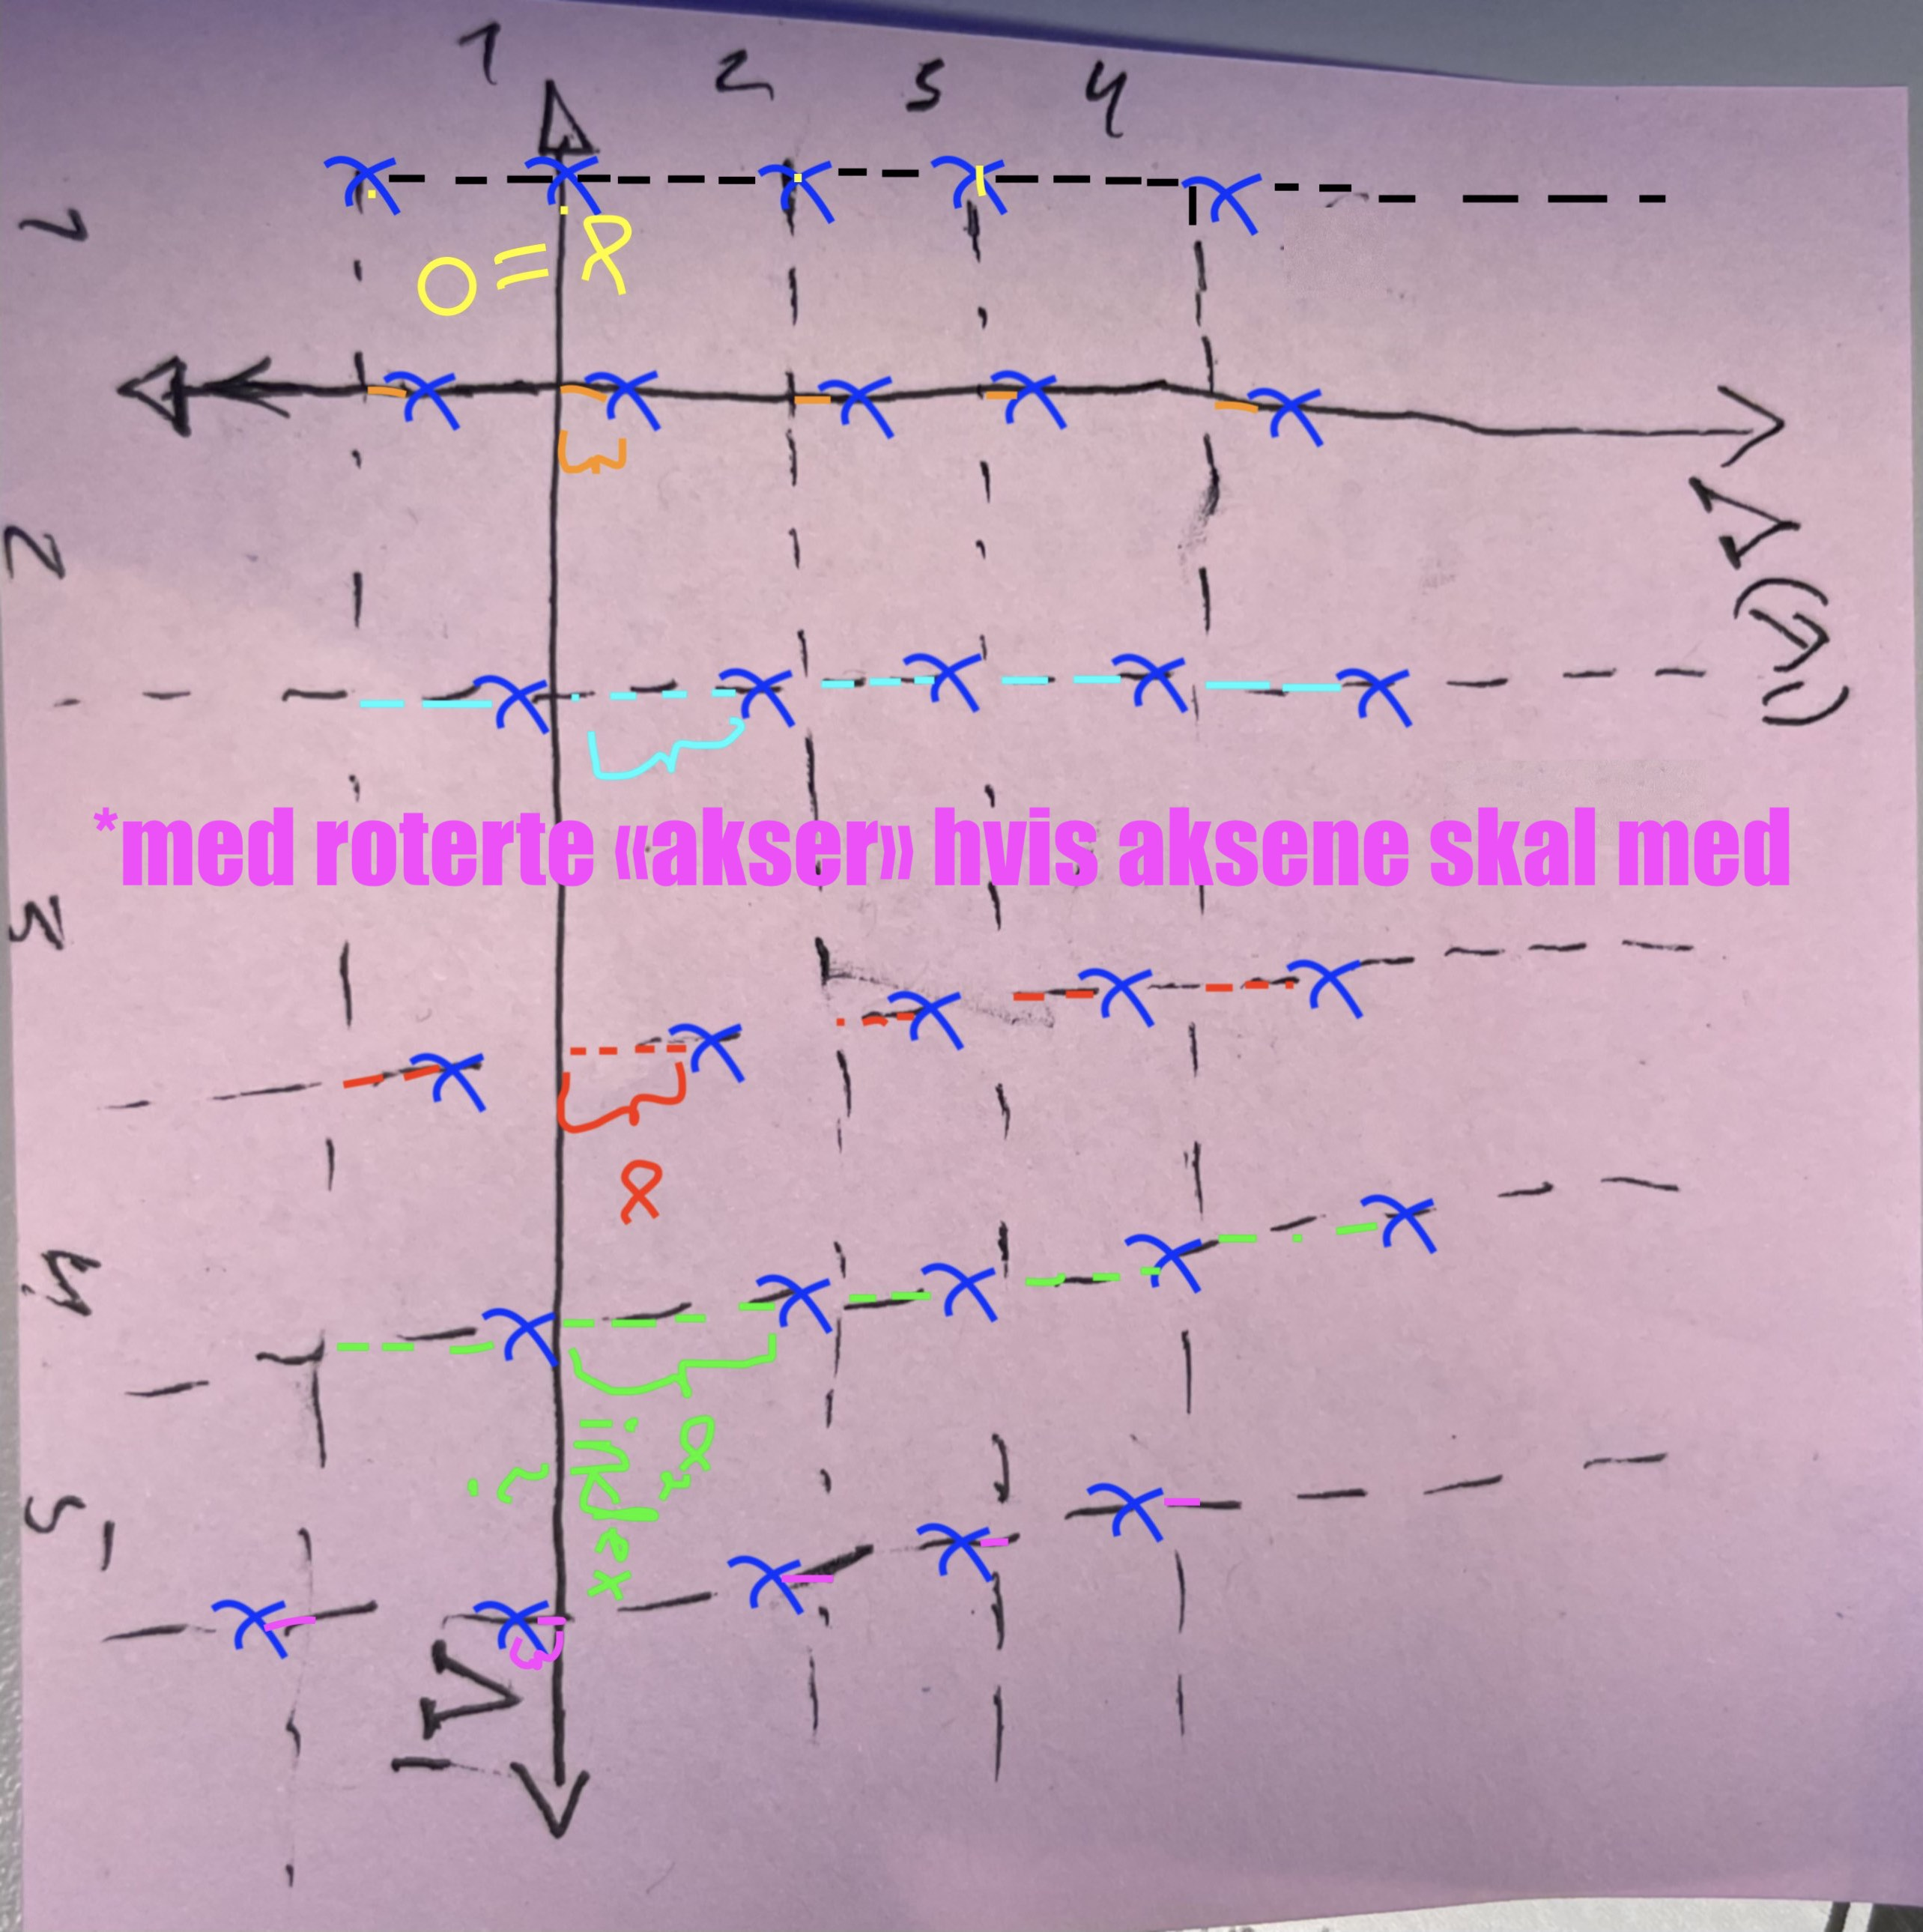
\includegraphics[width=0.9\linewidth]{multiple_shift_left_zero_horizontal.jpg}
    \end{subfigure}
\end{figure}



\begin{figure}[t]%h!
    \centering
    \begin{subfigure}{.47\textwidth}
        \centering
        %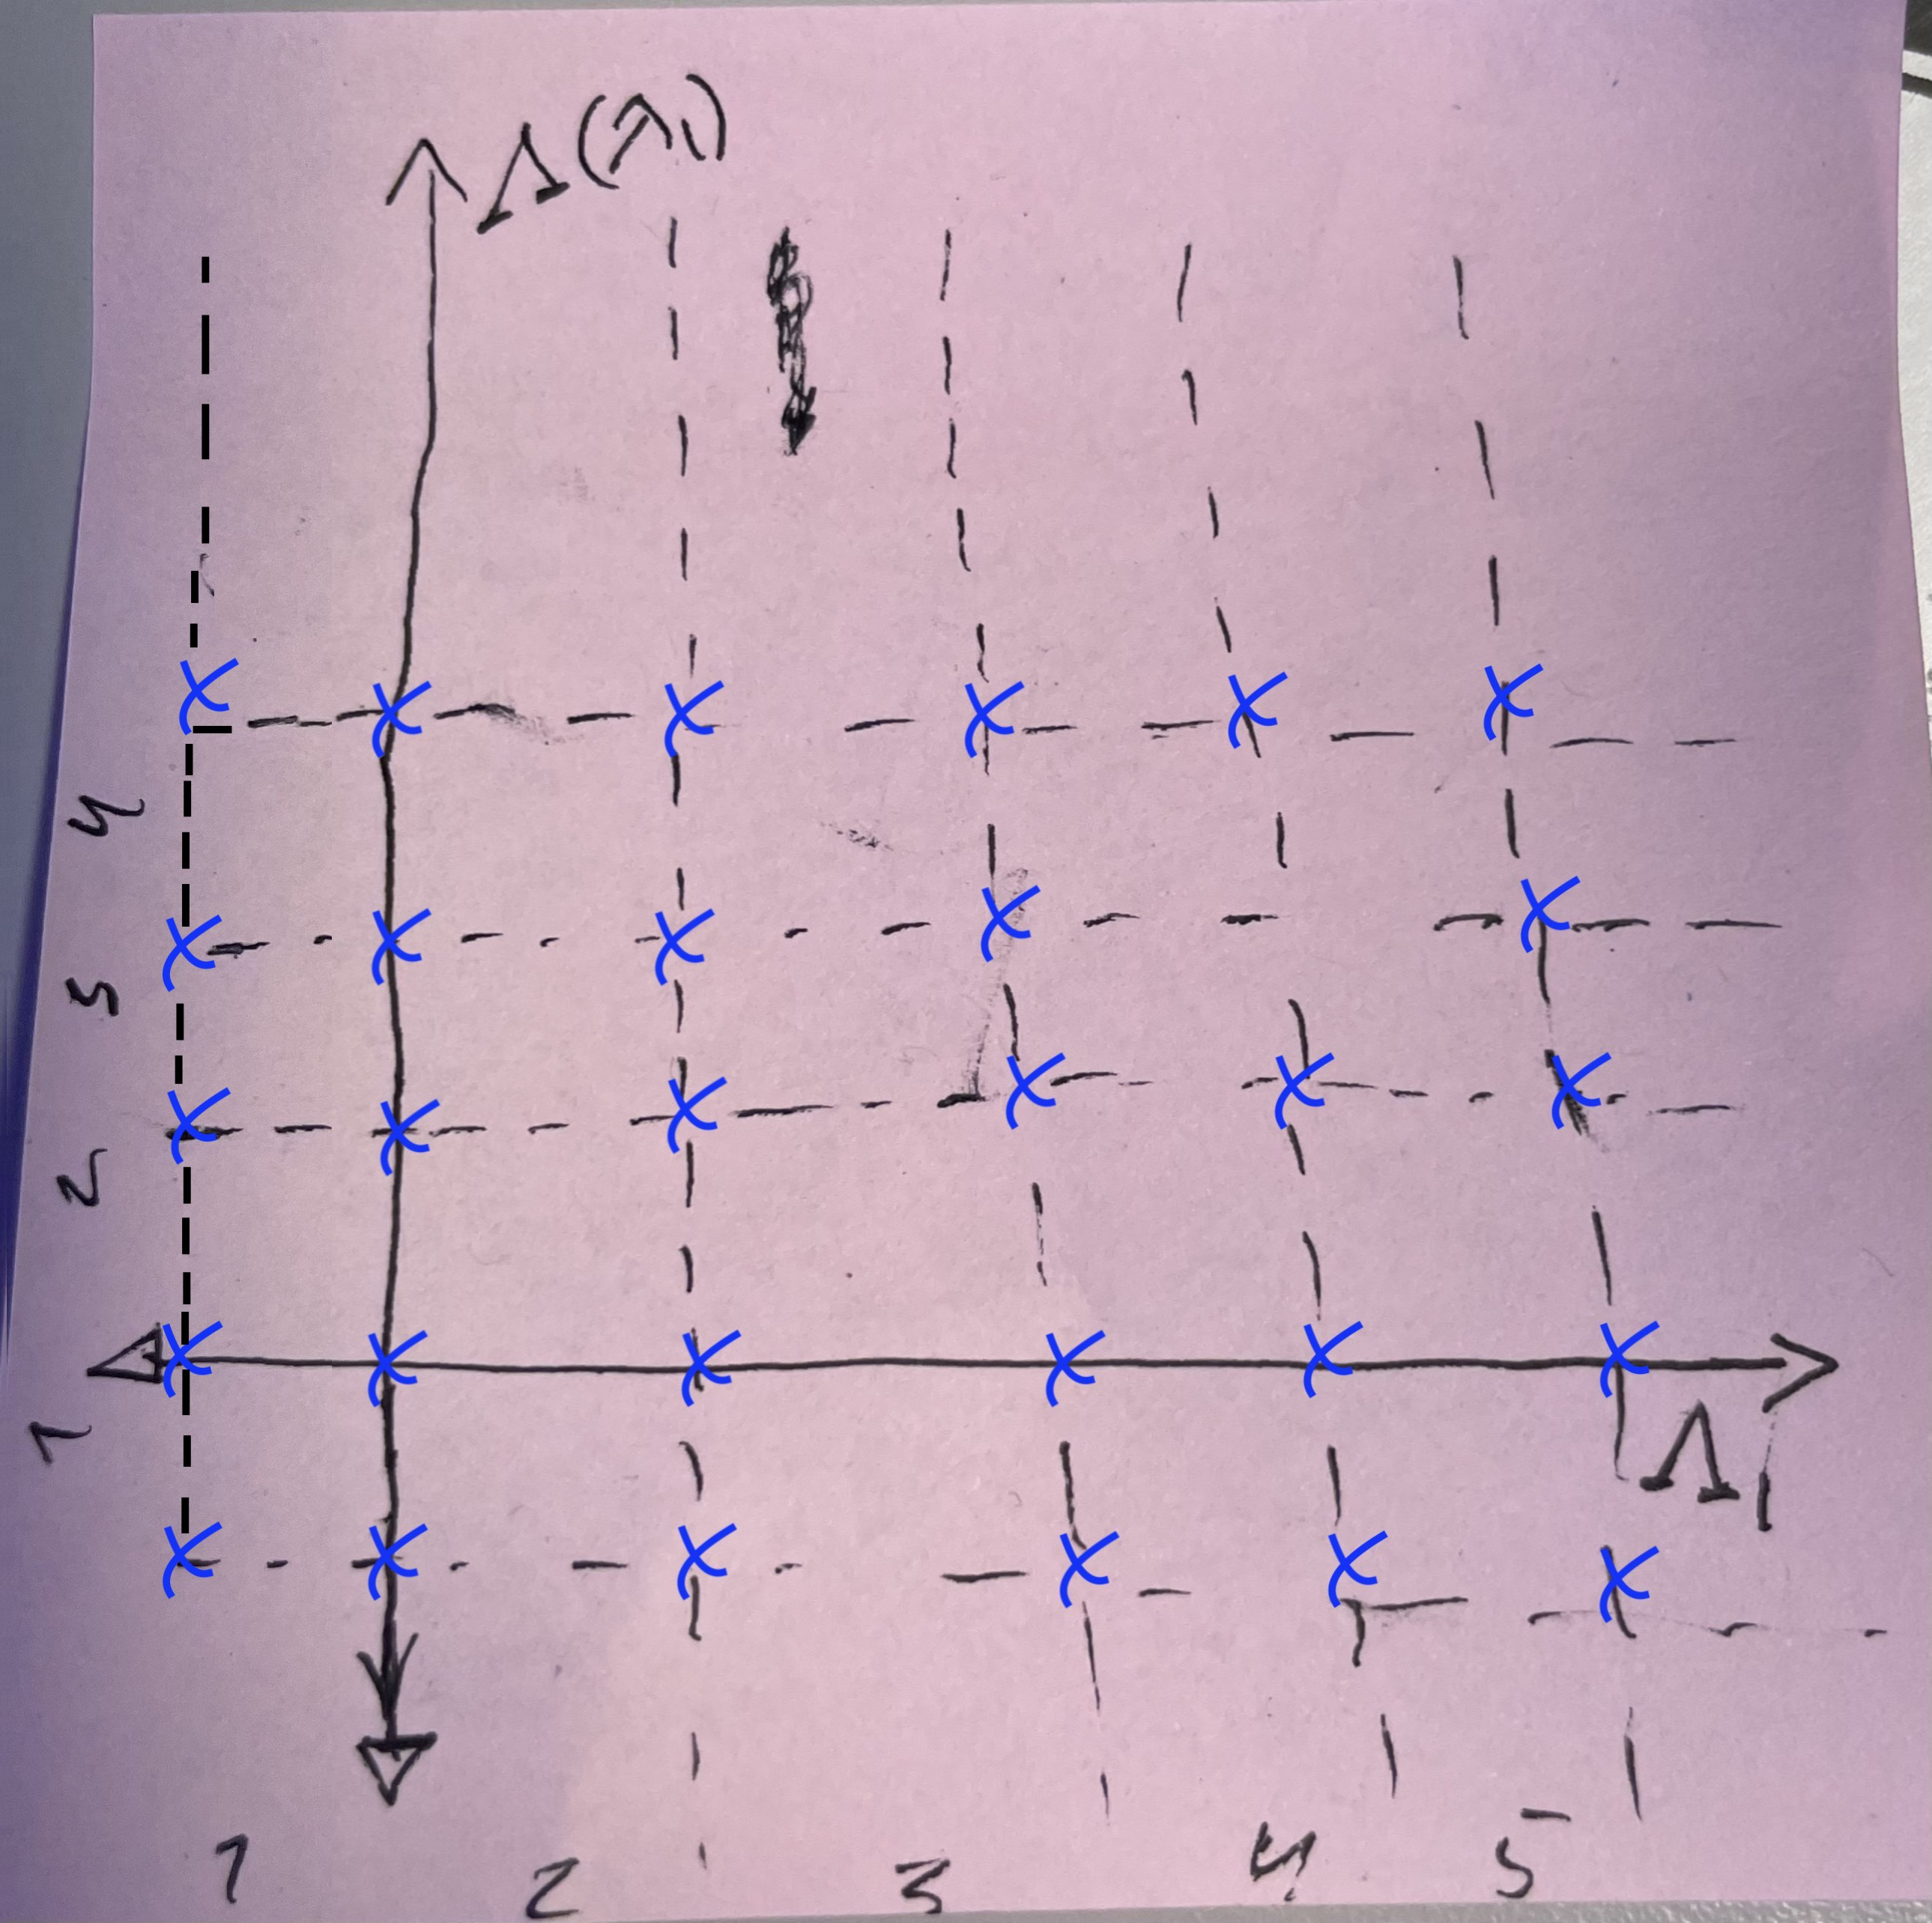
\includegraphics[width=0.9\linewidth]{spec_no_shift.jpg}
        %* Figure 1
        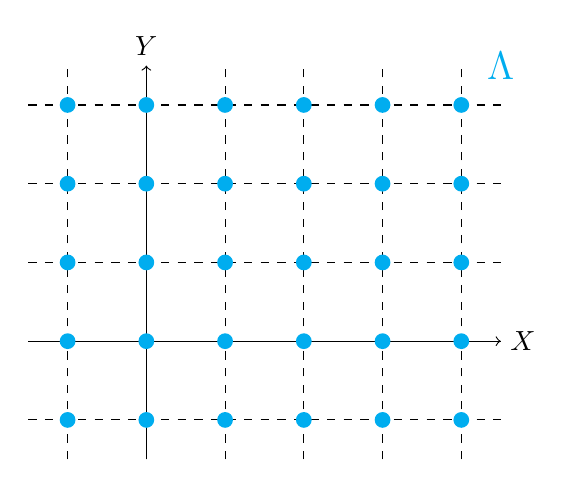
\begin{tikzpicture}
            \foreach \z in {0}{  % Controles whether the axes are inverted or not, 1 = yes, anything else = no
                

\ifnum\z=1
    % Axis lines
    %\draw[->] (-1.5,0) -- (4.5,0) node[right] {$\lambfuncGen{\lambda_2}$};
    %\draw[->] (0,-1.5) -- (0,3.5) node[above] {$\Lambda_2$};
    \draw[->] (-1.5,0) -- (4.5,0) node[right] {$Y$};
    \draw[->] (0,-1.5) -- (0,3.5) node[above] {$X$};

    % Dashed lines at each integer in the x direction
    \foreach \x in {-1,...,4}
        \draw[dashed] (\x,-1.5) -- (\x,3.5);

    % Dashed lines at each integer in the y direction
    \foreach \y in {-1,...,3}
        \draw[dashed] (-1.5,\y) -- (4.5,\y);
\else
    % Axis lines
    %\draw[->] (-1.5,0) -- (4.5,0) node[right] {$\Lambda_1$};
    %\draw[->] (0,-1.5) -- (0,3.5) node[above] {$\lambfunc$};
    \draw[->] (-1.5,0) -- (4.5,0) node[right] {$X$};
    \draw[->] (0,-1.5) -- (0,3.5) node[above] {$Y$};

    % Dashed lines at each integer in the x direction
    \foreach \x in {-1,...,4}
        \draw[dashed] (\x,-1.5) -- (\x,3.5);

    % Dashed lines at each integer in the y direction
    \foreach \y in {-1,...,3}
        \draw[dashed] (-1.5,\y) -- (4.5,\y);
\fi

% Lambda symbol in upper right corner
\node[cyan] at (4.5,3.5) {\Large $\Lambda$}; 
%\draw[orange] (4,3) node[above right] {$\Lambda$};
                % Cyan circles at an integer coordinate with no border
                \foreach \x in {-1,...,4}
                    \foreach \y in {-1,...,3}
                        \fill[cyan] (\x,\y) circle (0.1);
            }
        \end{tikzpicture}
        %* —————————————————
        \caption{Lattice spectra}
        \label{fig:lattice_spectra}
    \end{subfigure}\quad
    \begin{subfigure}{.47\textwidth}
        \centering
        %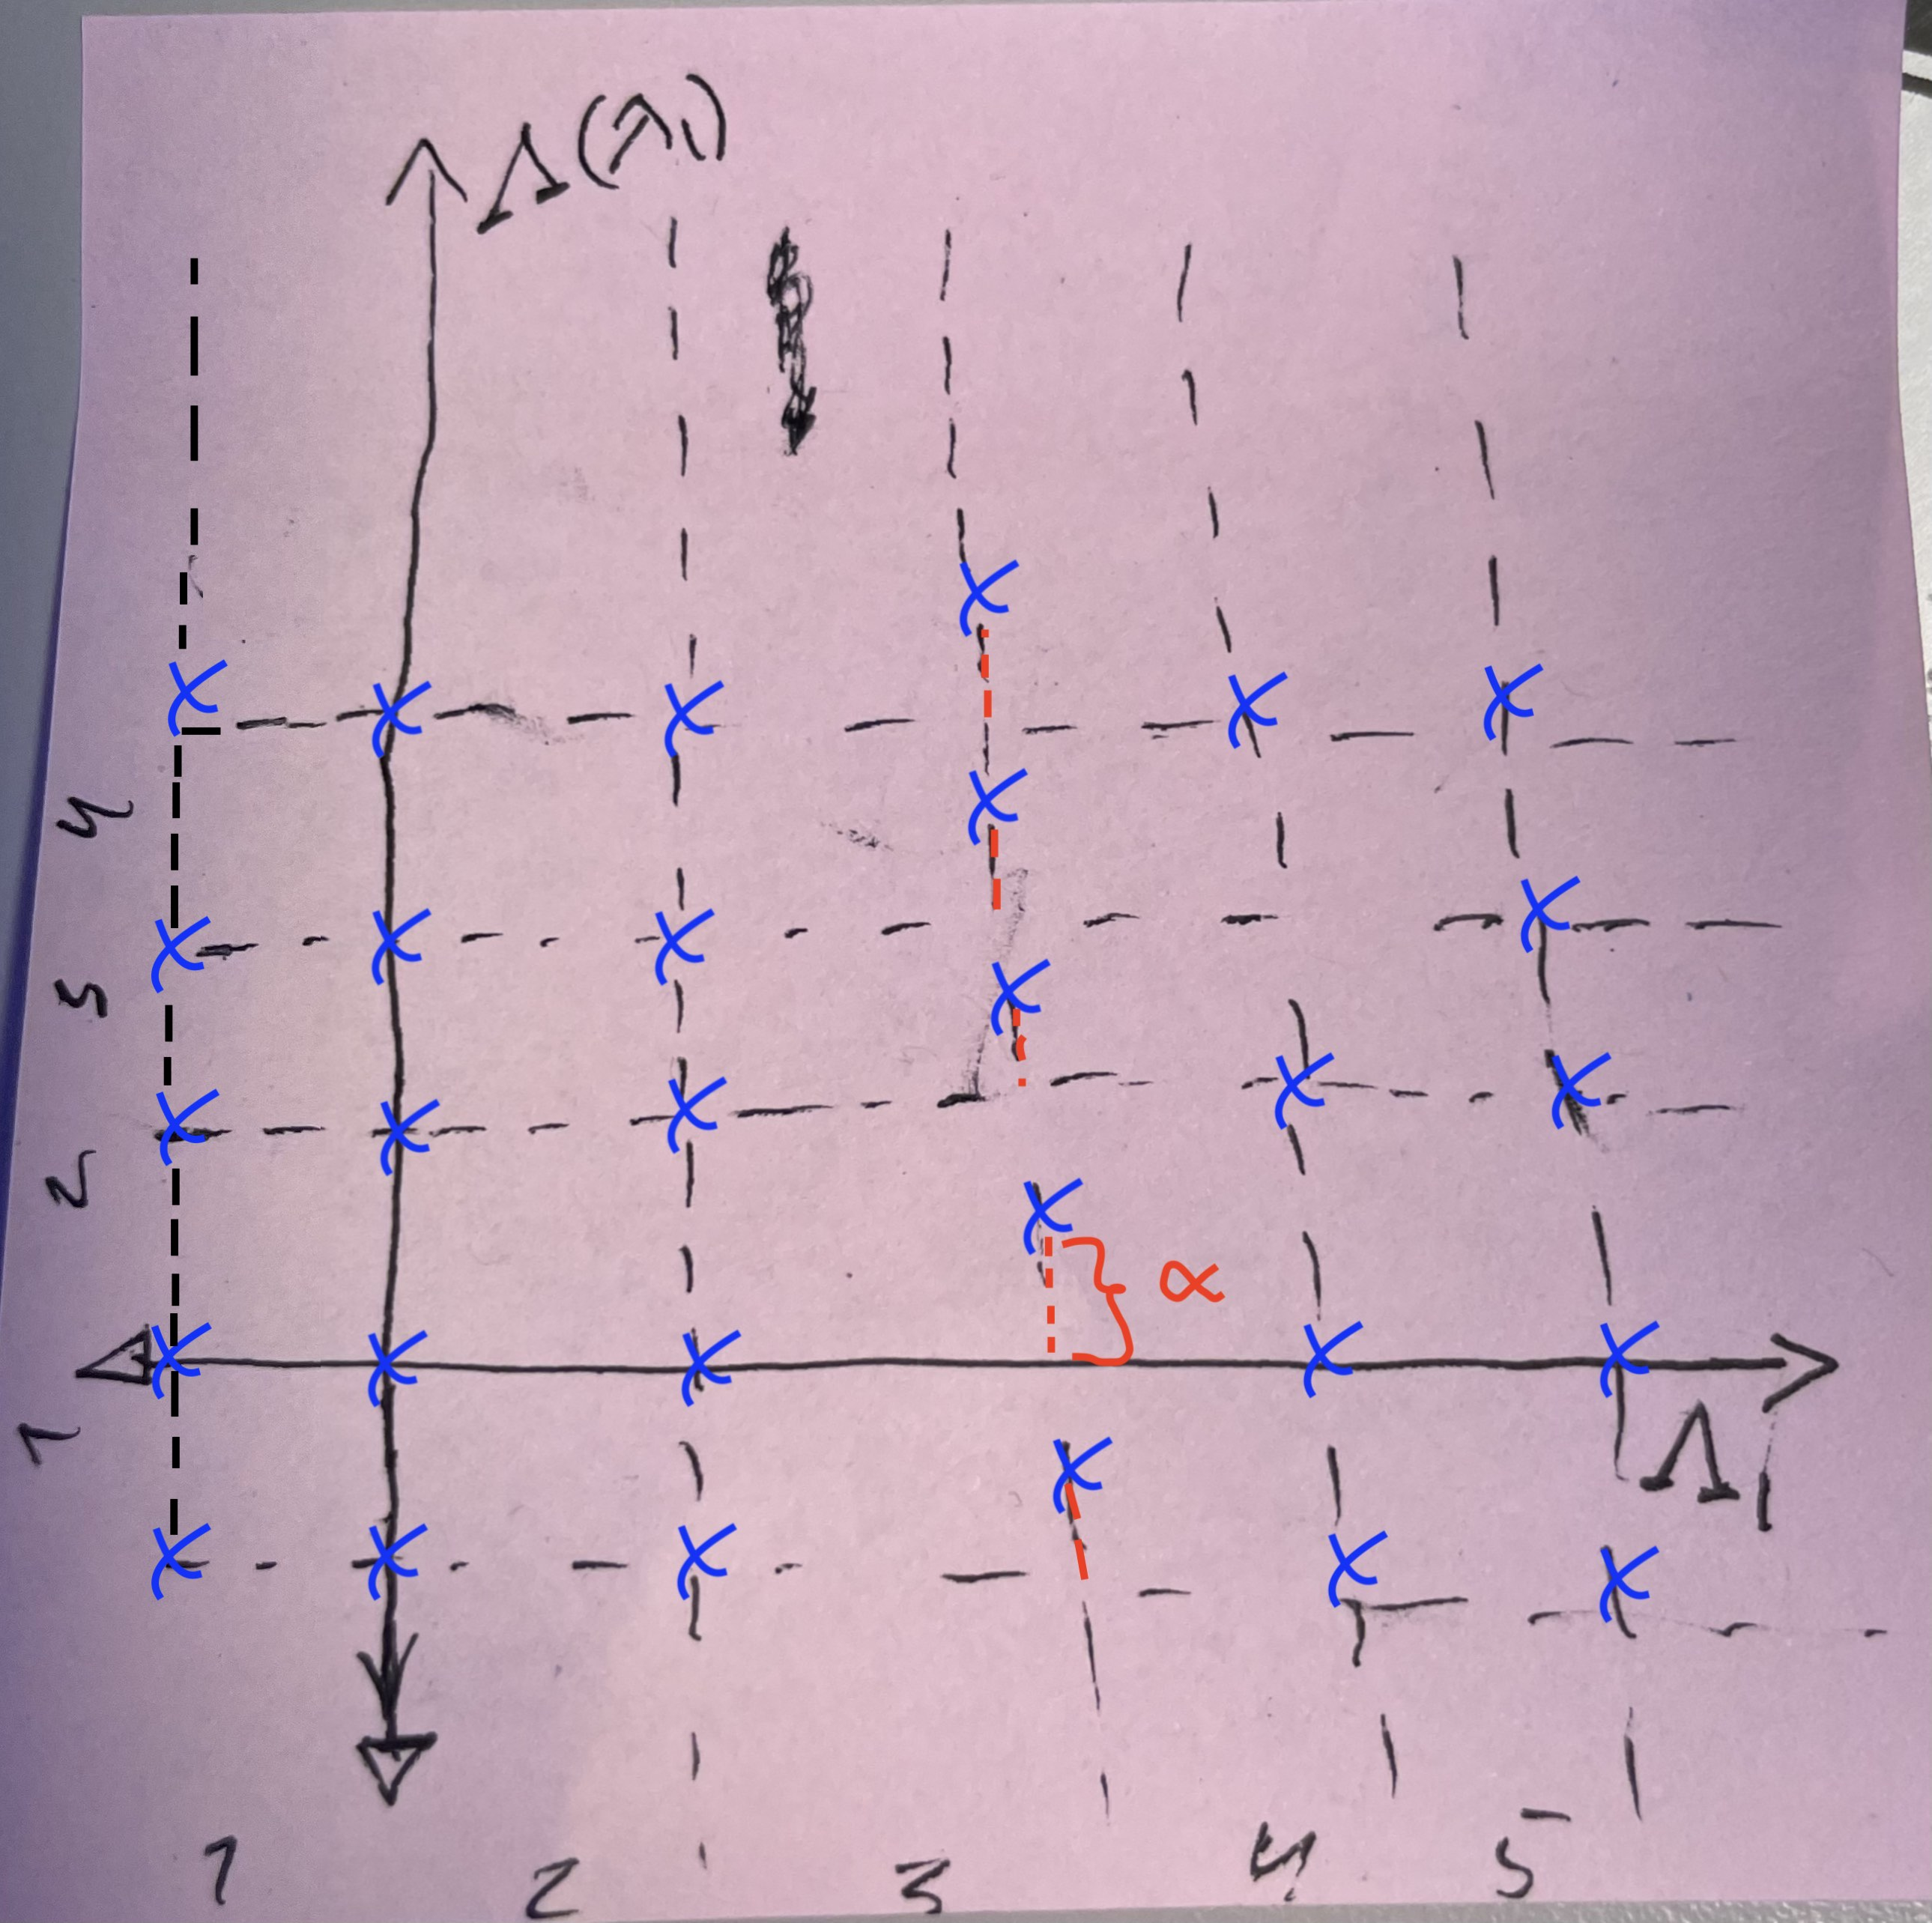
\includegraphics[width=0.9\linewidth]{spec_single_shift.jpg}
        %* Figure 2
        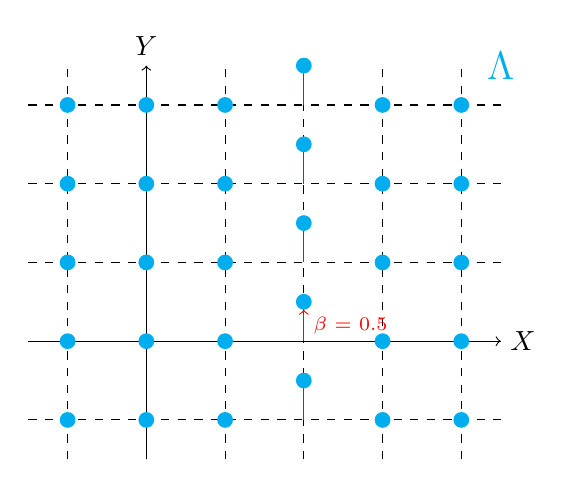
\begin{tikzpicture}
            \foreach \z in {0}{  % Controles whether the axes are inverted or not, 1 = yes, anything else = no
                

\ifnum\z=1
    % Axis lines
    %\draw[->] (-1.5,0) -- (4.5,0) node[right] {$\lambfuncGen{\lambda_2}$};
    %\draw[->] (0,-1.5) -- (0,3.5) node[above] {$\Lambda_2$};
    \draw[->] (-1.5,0) -- (4.5,0) node[right] {$Y$};
    \draw[->] (0,-1.5) -- (0,3.5) node[above] {$X$};

    % Dashed lines at each integer in the x direction
    \foreach \x in {-1,...,4}
        \draw[dashed] (\x,-1.5) -- (\x,3.5);

    % Dashed lines at each integer in the y direction
    \foreach \y in {-1,...,3}
        \draw[dashed] (-1.5,\y) -- (4.5,\y);
\else
    % Axis lines
    %\draw[->] (-1.5,0) -- (4.5,0) node[right] {$\Lambda_1$};
    %\draw[->] (0,-1.5) -- (0,3.5) node[above] {$\lambfunc$};
    \draw[->] (-1.5,0) -- (4.5,0) node[right] {$X$};
    \draw[->] (0,-1.5) -- (0,3.5) node[above] {$Y$};

    % Dashed lines at each integer in the x direction
    \foreach \x in {-1,...,4}
        \draw[dashed] (\x,-1.5) -- (\x,3.5);

    % Dashed lines at each integer in the y direction
    \foreach \y in {-1,...,3}
        \draw[dashed] (-1.5,\y) -- (4.5,\y);
\fi

% Lambda symbol in upper right corner
\node[cyan] at (4.5,3.5) {\Large $\Lambda$}; 
%\draw[orange] (4,3) node[above right] {$\Lambda$};
                % The single shift 
                \def\BetaSingle{0.5}

                % x in the range [-1,1]
                % Cyan circles at an integer coordinate with no border
                \foreach \x in {-1,...,1}
                \foreach \y in {-1,...,3}
                    \fill[cyan] (\x,\y) circle (0.1);  % Cyan circle
                    %\draw[fill=cyan] (\x,\y) circle (0.1);  % Black circle with cyan fill

                % x = 2
                \foreach \x in {2}{
                \foreach \y in {-1,...,3}{
                    \ifnum\y=0
                        %\draw[->, thick, red] (\x,\y) -- (\x,\y+\BetaSingle-0.1) node[midway, right] {\scriptsize $\beta$ = \BetaSingle};  % Line indicating the shift amount
                        \draw[->, red] (\x,\y) -- (\x,\y+\BetaSingle-0.1) node[midway, right] {\scriptsize $\beta$ = \BetaSingle};  % Line indicating the shift amount
                    \else
                        \draw[red] (\x,\y) -- (\x,\y+\BetaSingle);  % Line indicating the shift amount
                    \fi
                    \fill[cyan] (\x,\y+\BetaSingle) circle (0.1);  % Cyan circles at an integer coordinate with no border
                    %\draw[fill=cyan] (\x,\y+\BetaSingle) circle (0.1);  % Black circle with cyan fill
                }}

                % x in the range [3,4]
                % Cyan circles at an integer coordinate with no border
                \foreach \x in {3,...,4}{
                    \foreach \y in {-1,...,3}{
                        \fill[cyan] (\x,\y) circle (0.1);  % Cyan circle
                        %\draw[fill=cyan] (\x,\y) circle (0.1);  % Black circle with cyan fill
                }}
            }
        \end{tikzpicture}
        %* —————————————————
        \caption{Single vertical shift}
        \label{fig:single_shift_vertical}
    \end{subfigure}\\
    \begin{subfigure}{.47\textwidth}
        \centering
        %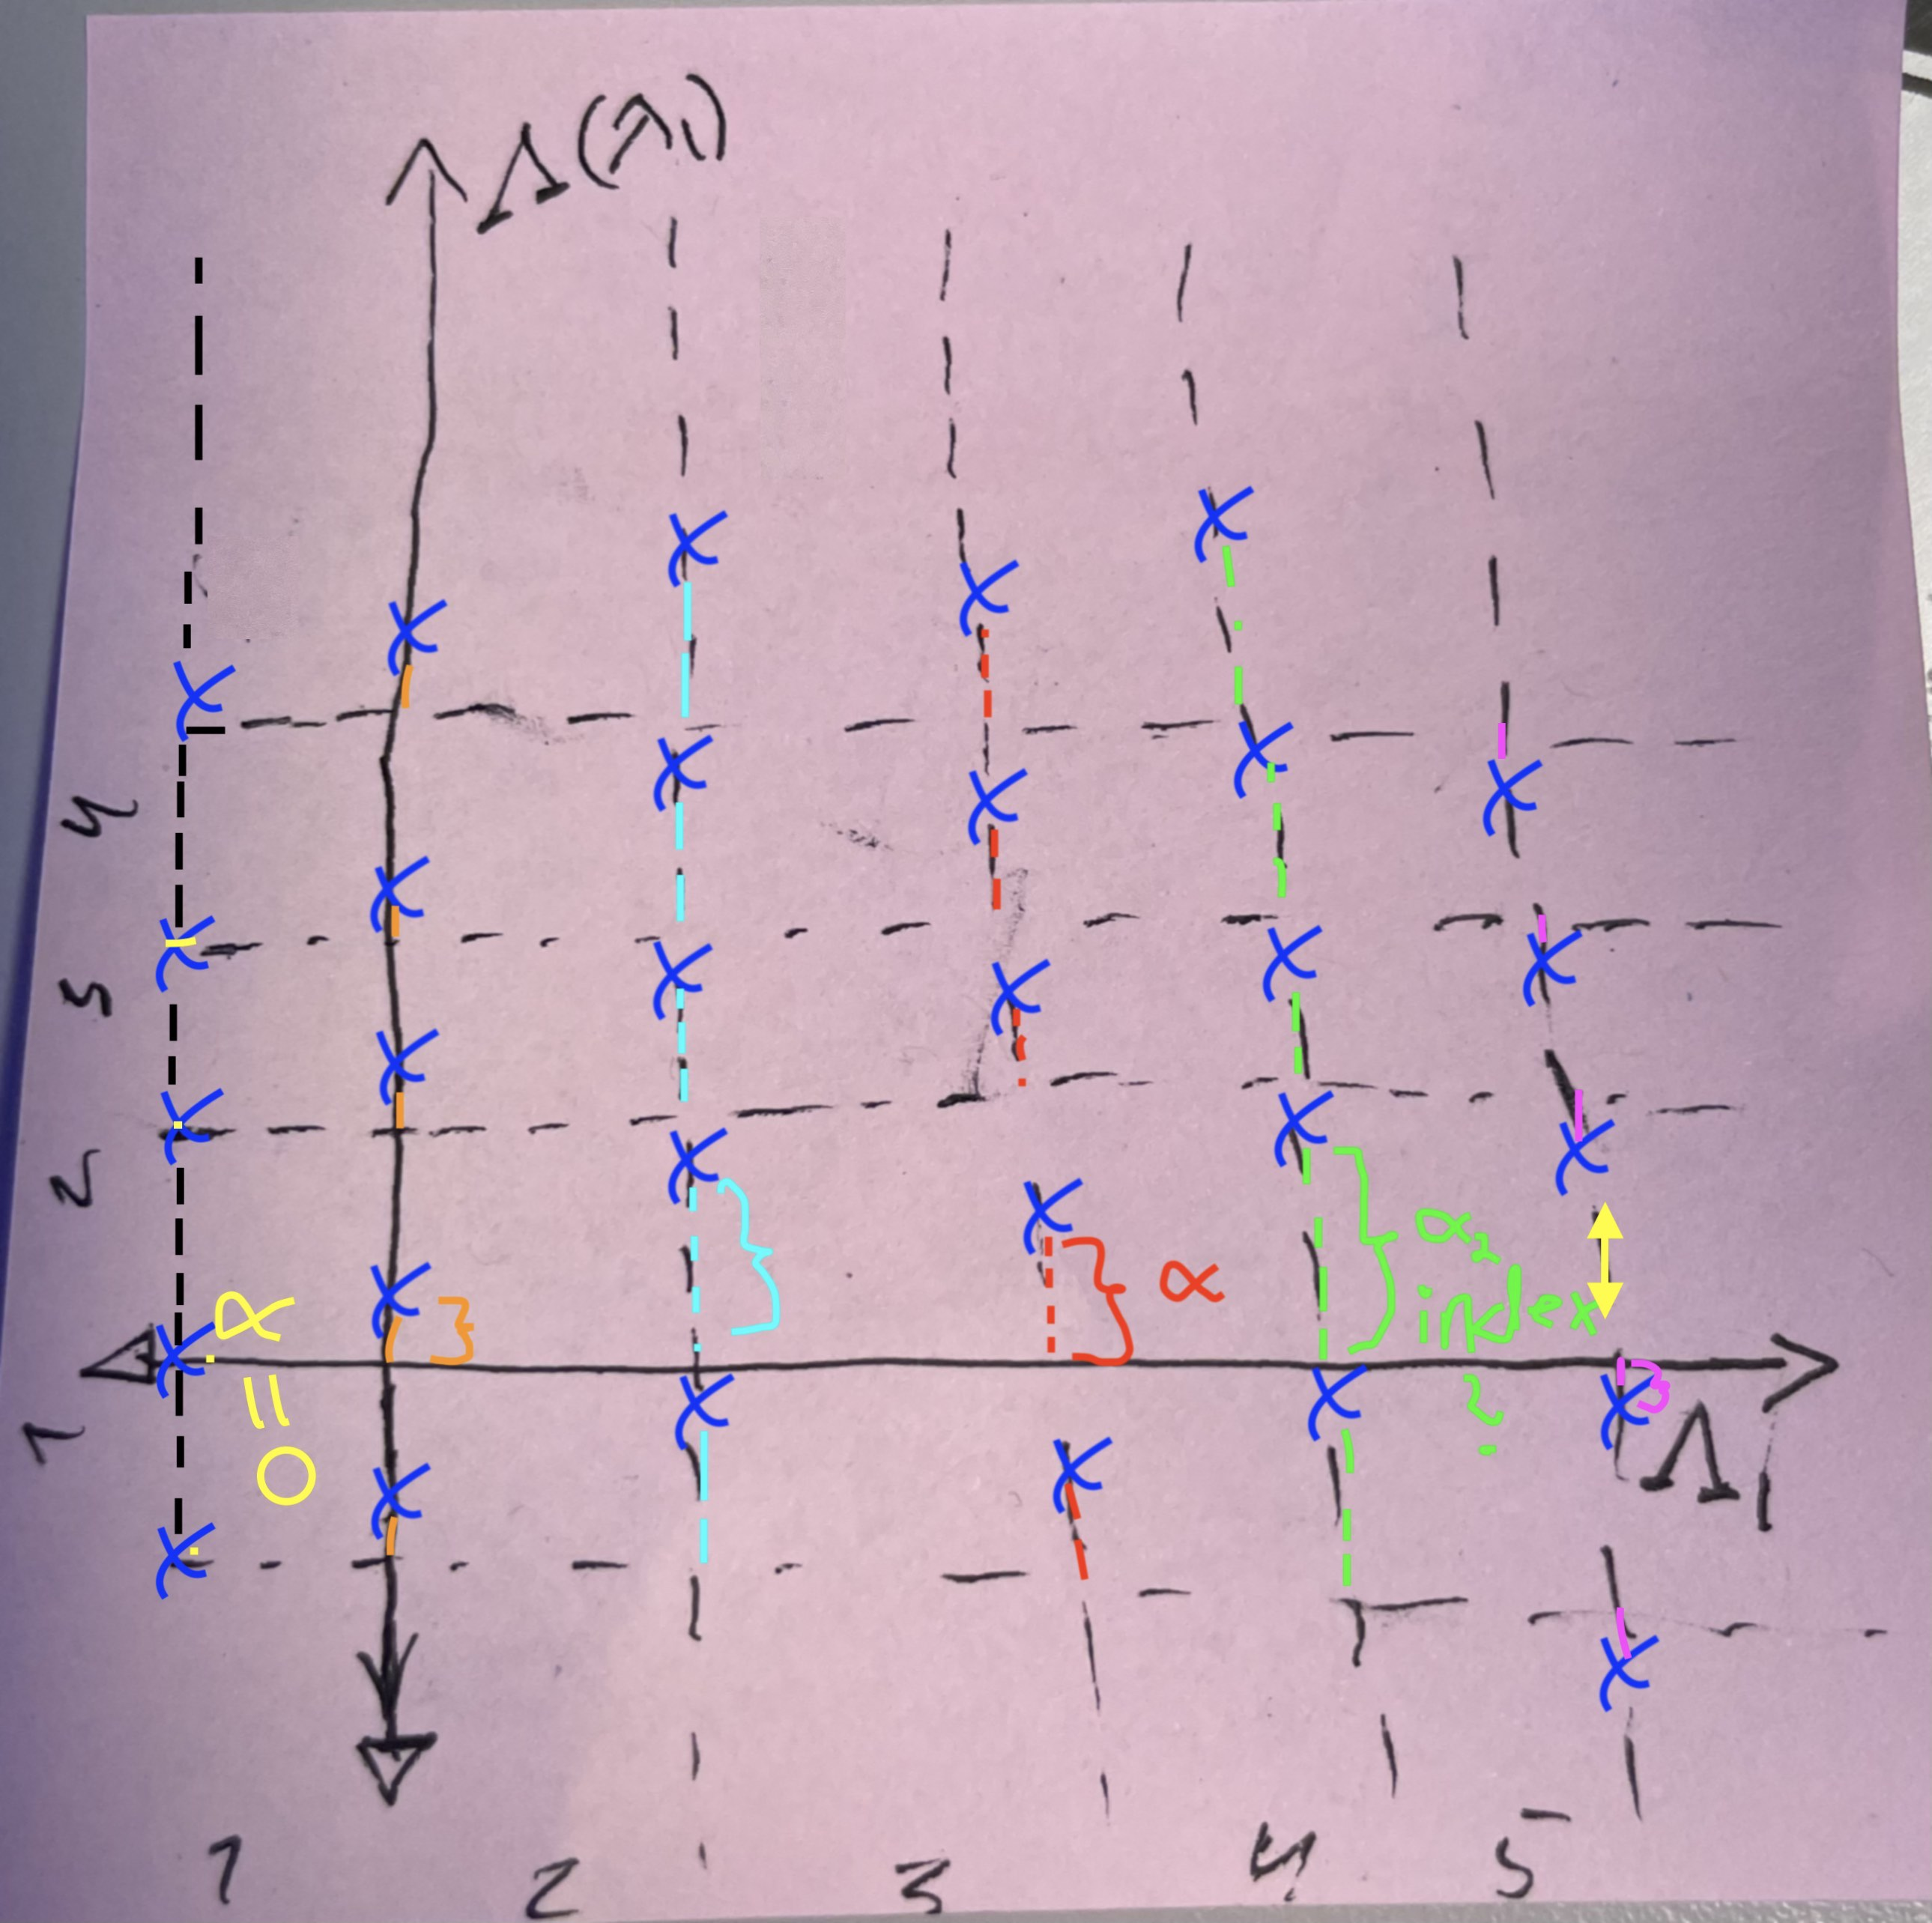
\includegraphics[width=0.9\linewidth]{multiple_shift_left_zero.jpg}
        %* Figure 3
        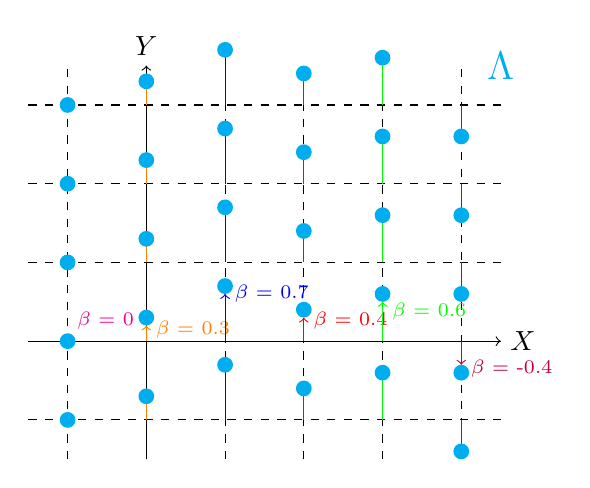
\begin{tikzpicture}
            \foreach \z in {0}{  % Controles whether the axes are inverted or not, 1 = yes, anything else = no
                

\ifnum\z=1
    % Axis lines
    %\draw[->] (-1.5,0) -- (4.5,0) node[right] {$\lambfuncGen{\lambda_2}$};
    %\draw[->] (0,-1.5) -- (0,3.5) node[above] {$\Lambda_2$};
    \draw[->] (-1.5,0) -- (4.5,0) node[right] {$Y$};
    \draw[->] (0,-1.5) -- (0,3.5) node[above] {$X$};

    % Dashed lines at each integer in the x direction
    \foreach \x in {-1,...,4}
        \draw[dashed] (\x,-1.5) -- (\x,3.5);

    % Dashed lines at each integer in the y direction
    \foreach \y in {-1,...,3}
        \draw[dashed] (-1.5,\y) -- (4.5,\y);
\else
    % Axis lines
    %\draw[->] (-1.5,0) -- (4.5,0) node[right] {$\Lambda_1$};
    %\draw[->] (0,-1.5) -- (0,3.5) node[above] {$\lambfunc$};
    \draw[->] (-1.5,0) -- (4.5,0) node[right] {$X$};
    \draw[->] (0,-1.5) -- (0,3.5) node[above] {$Y$};

    % Dashed lines at each integer in the x direction
    \foreach \x in {-1,...,4}
        \draw[dashed] (\x,-1.5) -- (\x,3.5);

    % Dashed lines at each integer in the y direction
    \foreach \y in {-1,...,3}
        \draw[dashed] (-1.5,\y) -- (4.5,\y);
\fi

% Lambda symbol in upper right corner
\node[cyan] at (4.5,3.5) {\Large $\Lambda$}; 
%\draw[orange] (4,3) node[above right] {$\Lambda$};
                % Shift list
                \def\BetaMinOne{0}
                \def\BetaZero{0.3}
                \def\BetaOne{0.7}
                \def\BetaTwo{0.4}
                \def\BetaThree{0.6}
                \def\BetaFour{-0.4}

                % x = -1
                \foreach \x in {-1}{
                \foreach \y in {-1,...,3}{
                    \ifnum\y=0
                    \draw[->, magenta] (\x,\y) -- (\x,\y+0.05\BetaMinOne) node[midway, above right] {\scriptsize $\beta$ = \BetaMinOne};  % Line indicating the shift amount
                    \else
                    \draw[magenta] (\x,\y) -- (\x,\y+\BetaMinOne);  % Line indicating the shift amount
                    \fi
                    \fill[cyan] (\x,\y+\BetaMinOne) circle (0.1);  % Cyan circles at an integer coordinate with no border
                }}
                % x = 0
                \foreach \x in {0}{
                \foreach \y in {-1,...,3}{
                    \ifnum\y=0
                    \draw[->, orange] (\x,\y) -- (\x,\y+\BetaZero-0.1) node[near end, right] {\scriptsize $\beta$ = \BetaZero};  % Line indicating the shift amount
                    \else
                    \draw[orange] (\x,\y) -- (\x,\y+\BetaZero);  % Line indicating the shift amount
                    \fi
                    \fill[cyan] (\x,\y+\BetaZero) circle (0.1);  % Cyan circles at an integer coordinate with no border
                }}
                % x = 1
                \foreach \x in {1}{
                \foreach \y in {-1,...,3}{
                    \ifnum\y=0
                    \draw[->, blue] (\x,\y) -- (\x,\y+\BetaOne-0.1) node[at end, right] {\scriptsize $\beta$ = \BetaOne};  % Line indicating the shift amount
                    \else
                    \draw[blue] (\x,\y) -- (\x,\y+\BetaOne);  % Line indicating the shift amount
                    \fi
                    \fill[cyan] (\x,\y+\BetaOne) circle (0.1);  % Cyan circles at an integer coordinate with no border
                }}
                % x = 2
                \foreach \x in {2}{
                \foreach \y in {-1,...,3}{
                    \ifnum\y=0
                    \draw[->, red] (\x,\y) -- (\x,\y+\BetaTwo-0.1) node[very near end, right] {\scriptsize $\beta$ = \BetaTwo};  % Line indicating the shift amount
                    \else
                    \draw[red] (\x,\y) -- (\x,\y+\BetaTwo);  % Line indicating the shift amount
                    \fi
                    \fill[cyan] (\x,\y+\BetaTwo) circle (0.1);  % Cyan circles at an integer coordinate with no border
                }}
                % x = 3
                \foreach \x in {3}{
                \foreach \y in {-1,...,3}{
                    \ifnum\y=0
                    \draw[->, green] (\x,\y) -- (\x,\y+\BetaThree-0.1) node[near end, right] {\scriptsize $\beta$ = \BetaThree};  % Line indicating the shift amount
                    \else
                    \draw[green] (\x,\y) -- (\x,\y+\BetaThree);  % Line indicating the shift amount
                    \fi
                    \fill[cyan] (\x,\y+\BetaThree) circle (0.1);  % Cyan circles at an integer coordinate with no border
                }}
                % x = 4
                \foreach \x in {4}{
                \foreach \y in {-1,...,3}{
                    \ifnum\y=0
                    \draw[->, purple] (\x,\y) -- (\x,\y+\BetaFour+0.1) node[at end, right, yshift=-0.5mm] {\scriptsize $\beta$ = \BetaFour};  % Line indicating the shift amount
                    \else
                    \draw[purple] (\x,\y) -- (\x,\y+\BetaFour);  % Line indicating the shift amount
                    \fi
                    \fill[cyan] (\x,\y+\BetaFour) circle (0.1);  % Cyan circles at an integer coordinate with no border
                }}
            }
        \end{tikzpicture}
        %* —————————————————
        \caption{Multiple individual vertical shifts}
        \label{fig:multiple_shift_vertical}
    \end{subfigure}\quad
    \begin{subfigure}{.47\textwidth}
        \centering
        %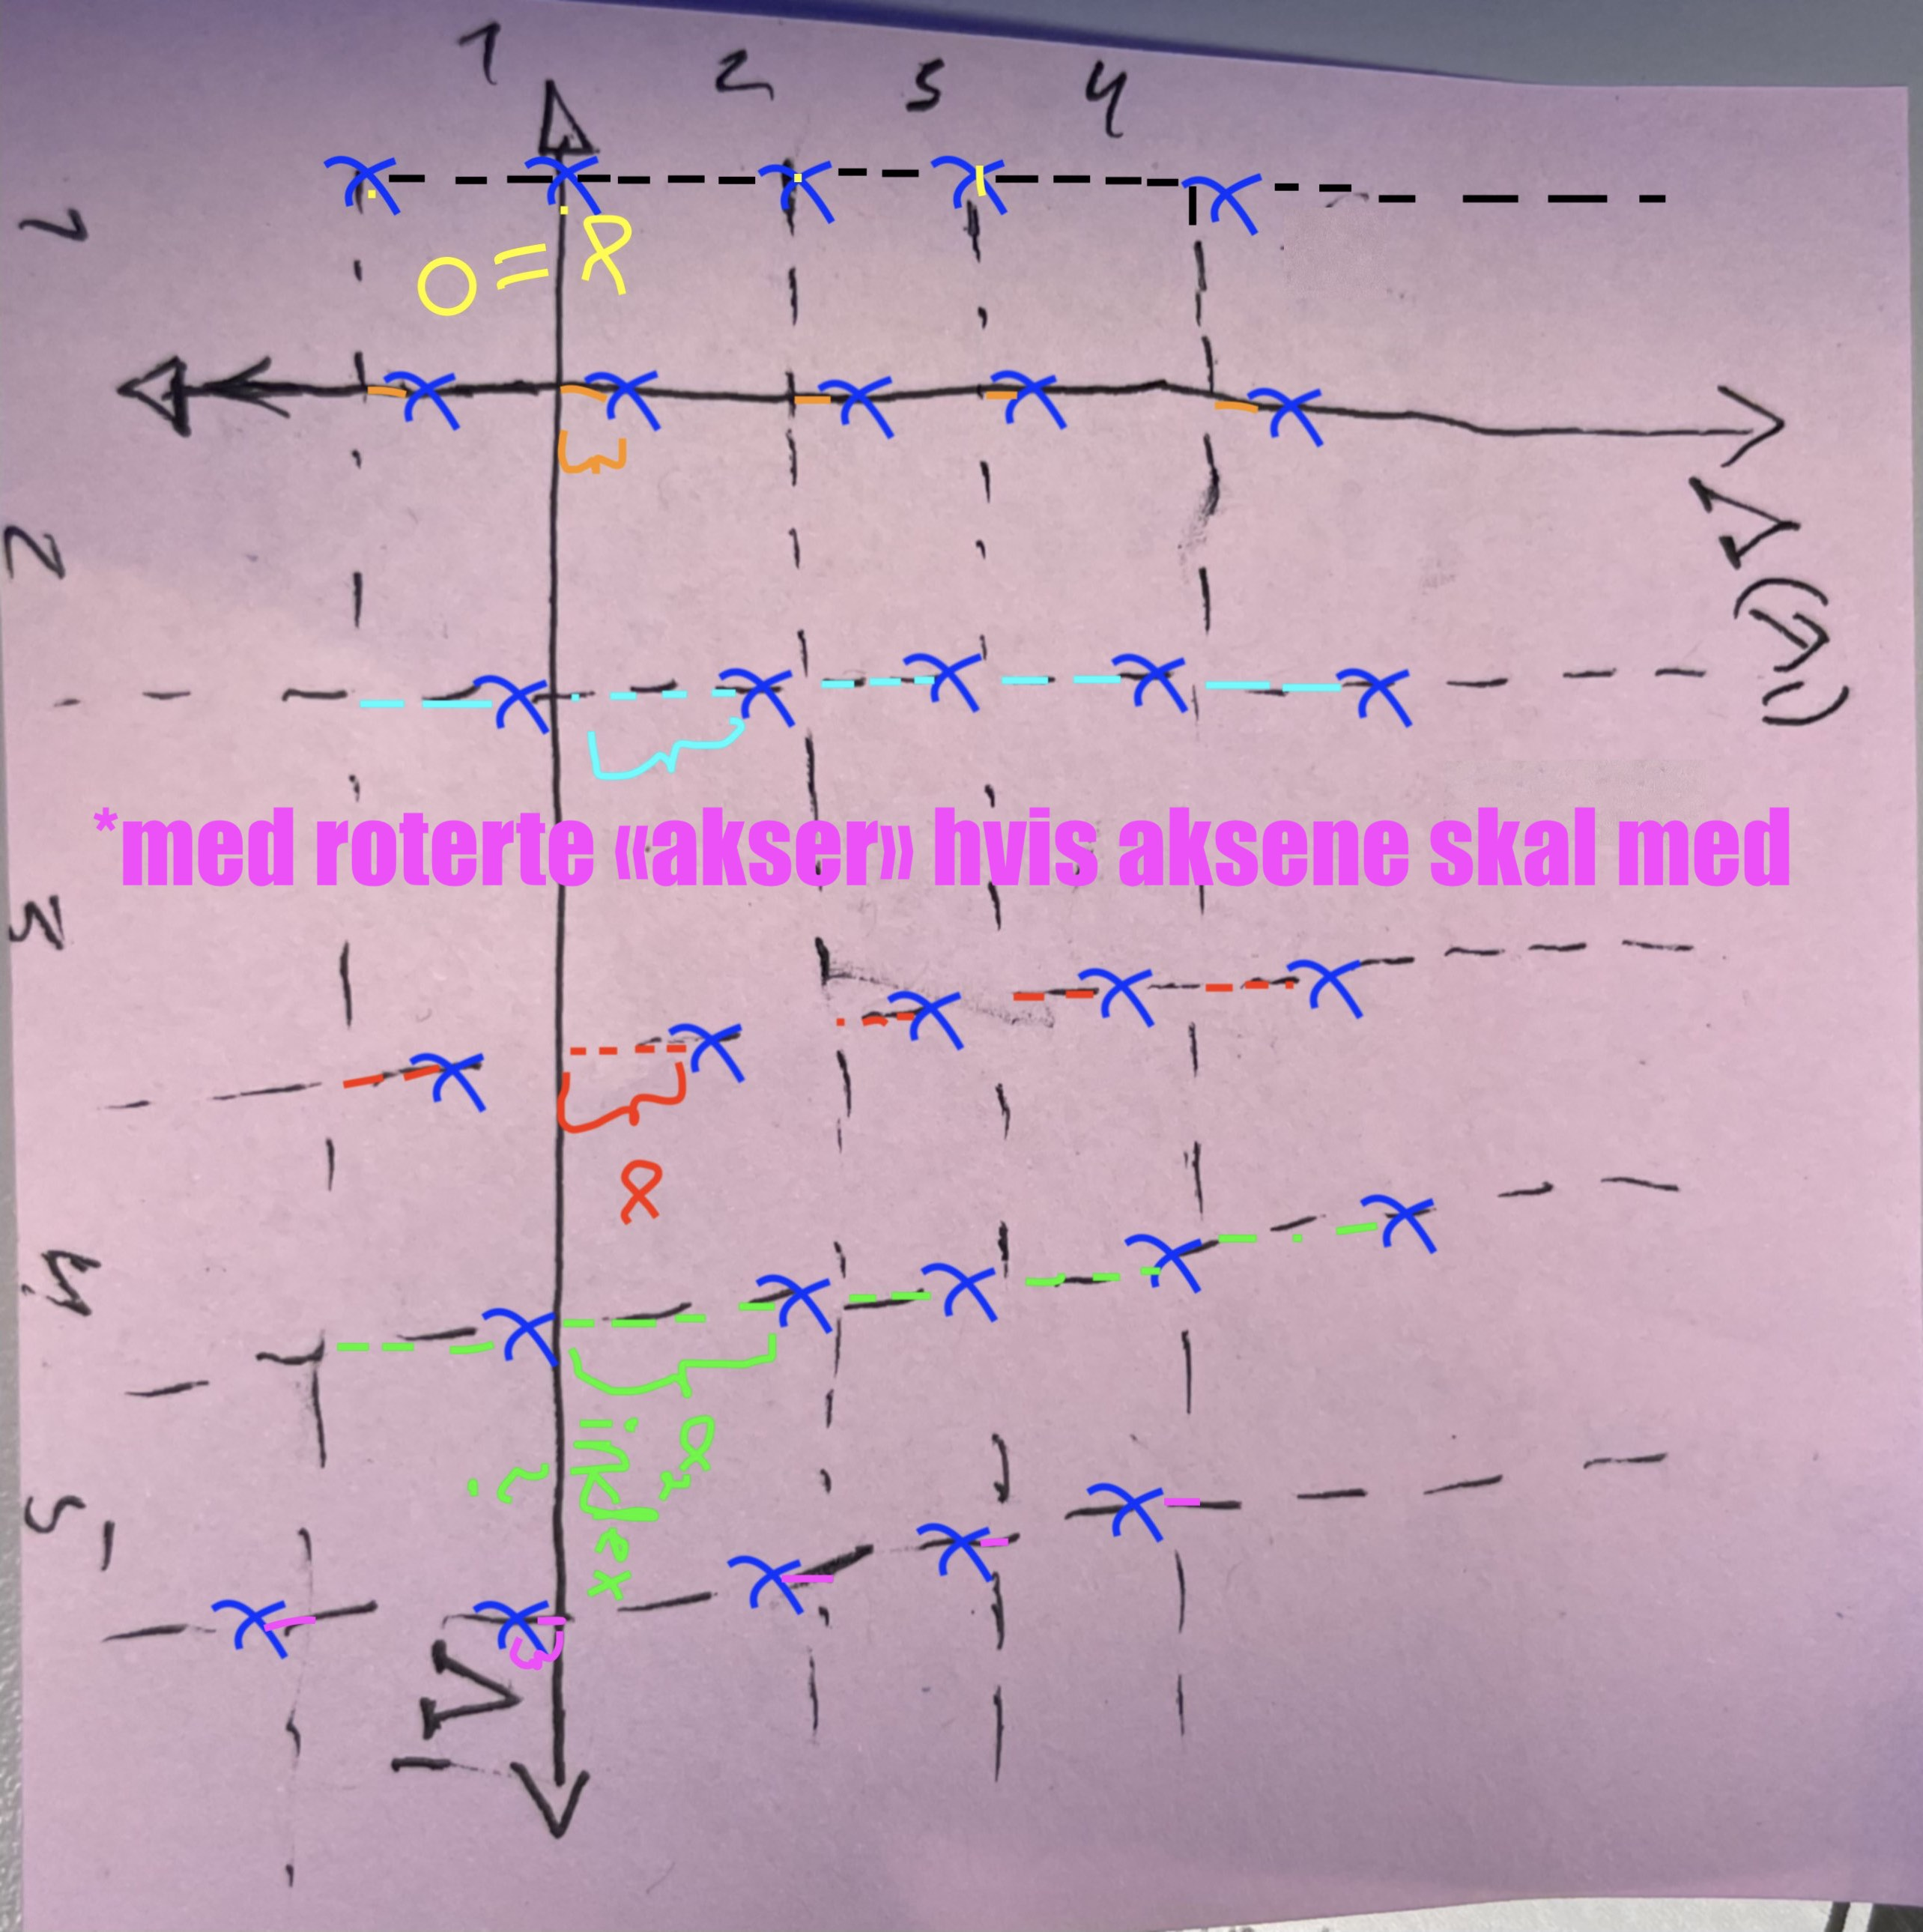
\includegraphics[width=0.9\linewidth]{multiple_shift_left_zero_horizontal.jpg}
        %* Figure 4
        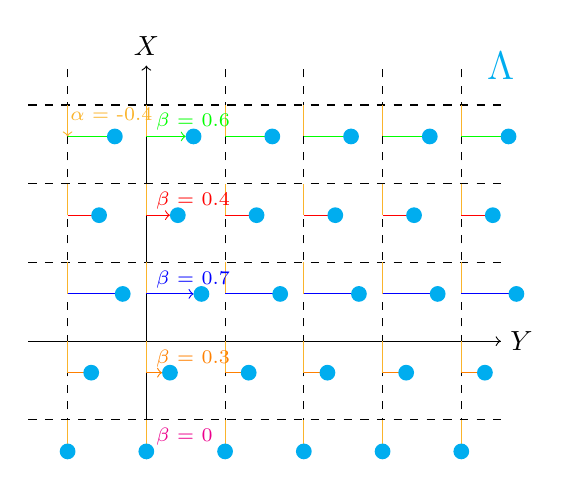
\begin{tikzpicture}
            \foreach \z in {1}{  % Controles whether the axes are inverted or not, 1 = yes, anything else = no
                

\ifnum\z=1
    % Axis lines
    %\draw[->] (-1.5,0) -- (4.5,0) node[right] {$\lambfuncGen{\lambda_2}$};
    %\draw[->] (0,-1.5) -- (0,3.5) node[above] {$\Lambda_2$};
    \draw[->] (-1.5,0) -- (4.5,0) node[right] {$Y$};
    \draw[->] (0,-1.5) -- (0,3.5) node[above] {$X$};

    % Dashed lines at each integer in the x direction
    \foreach \x in {-1,...,4}
        \draw[dashed] (\x,-1.5) -- (\x,3.5);

    % Dashed lines at each integer in the y direction
    \foreach \y in {-1,...,3}
        \draw[dashed] (-1.5,\y) -- (4.5,\y);
\else
    % Axis lines
    %\draw[->] (-1.5,0) -- (4.5,0) node[right] {$\Lambda_1$};
    %\draw[->] (0,-1.5) -- (0,3.5) node[above] {$\lambfunc$};
    \draw[->] (-1.5,0) -- (4.5,0) node[right] {$X$};
    \draw[->] (0,-1.5) -- (0,3.5) node[above] {$Y$};

    % Dashed lines at each integer in the x direction
    \foreach \x in {-1,...,4}
        \draw[dashed] (\x,-1.5) -- (\x,3.5);

    % Dashed lines at each integer in the y direction
    \foreach \y in {-1,...,3}
        \draw[dashed] (-1.5,\y) -- (4.5,\y);
\fi

% Lambda symbol in upper right corner
\node[cyan] at (4.5,3.5) {\Large $\Lambda$}; 
%\draw[orange] (4,3) node[above right] {$\Lambda$};
                % Shift list
                \def\BetaMinOne{0}
                \def\BetaZero{0.3}
                \def\BetaOne{0.7}
                \def\BetaTwo{0.4}
                \def\BetaThree{0.6}
                \def\BetaFour{-0.6}
                \def\AlphaONE{-0.4}

                % The X shift lines at x=0
                \foreach \x in {-1,...,4}{
                \foreach \y in {-1,...,3}{
                    \ifnum\x=-1
                        \ifnum\y=3
                            \draw[->, Dandelion] (\x,\y) -- (\x,\y+\AlphaONE) node[pos=0.3, right, xshift=-0.9mm] {\scriptsize $\alpha$ = \AlphaONE};  % Line indicating the shift amount
                        \else
                            %\draw[->, thick, purple] (\x,\y) -- (\x,\y+\AlphaONE);  % Line indicating the shift amount
                            \draw[Dandelion] (\x,\y) -- (\x,\y+\AlphaONE);  % Line indicating the shift amount
                        \fi
                    \else
                    \draw[Dandelion] (\x,\y) -- (\x,\y+\AlphaONE);  % Line indicating the shift amount
                    \fi
                }}

                % The Y shift
                % y = -1
                \foreach \y in {-1}{
                \foreach \x in {-1,...,4}{
                    \ifnum\x=0
                    \draw[->, magenta] (\x,\y+\AlphaONE) -- (\x+\BetaMinOne+0.05, \y+\AlphaONE) node[at start, above right, yshift=-0.5mm] {\scriptsize $\beta$ = \BetaMinOne};  % Line indicating the shift amount
                    \else
                    \draw[magenta] (\x,\y+\AlphaONE) -- (\x+\BetaMinOne,\y+\AlphaONE);  % Line indicating the shift amount
                    \fi
                    \fill[cyan] (\x+\BetaMinOne,\y+\AlphaONE) circle (0.1);  % Cyan circles at an integer coordinate with no border
                }}
                % y = 0
                \foreach \y in {0}{
                \foreach \x in {-1,...,4}{
                    \ifnum\x=0
                    \draw[->, orange] (\x,\y+\AlphaONE) -- (\x+\BetaZero-0.1,\y+\AlphaONE) node[at start, above right, yshift=-0.5mm] {\scriptsize $\beta$ = \BetaZero};  % Line indicating the shift amount
                    \else
                    \draw[orange] (\x,\y+\AlphaONE) -- (\x+\BetaZero,\y+\AlphaONE);  % Line indicating the shift amount
                    \fi
                    \fill[cyan] (\x+\BetaZero,\y+\AlphaONE) circle (0.1);  % Cyan circles at an integer coordinate with no border
                }}
                % y = 1
                \foreach \y in {1}{
                \foreach \x in {-1,...,4}{
                    \ifnum\x=0
                    \draw[->, blue] (\x,\y+\AlphaONE) -- (\x+\BetaOne-0.1,\y+\AlphaONE) node[at start, above right, yshift=-0.5mm] {\scriptsize $\beta$ = \BetaOne};  % Line indicating the shift amount
                    \else
                    \draw[blue] (\x,\y+\AlphaONE) -- (\x+\BetaOne,\y+\AlphaONE);  % Line indicating the shift amount
                    \fi
                    \fill[cyan] (\x+\BetaOne,\y+\AlphaONE) circle (0.1);  % Cyan circles at an integer coordinate with no border
                }}
                % y = 2
                \foreach \y in {2}{
                \foreach \x in {-1,...,4}{
                    \ifnum\x=0
                    \draw[->, red] (\x,\y+\AlphaONE) -- (\x+\BetaTwo-0.1,\y+\AlphaONE) node[at start, above right, yshift=-0.5mm] {\scriptsize $\beta$ = \BetaTwo};  % Line indicating the shift amount
                    \else
                    \draw[red] (\x,\y+\AlphaONE) -- (\x+\BetaTwo,\y+\AlphaONE);  % Line indicating the shift amount
                    \fi
                    \fill[cyan] (\x+\BetaTwo,\y+\AlphaONE) circle (0.1);  % Cyan circles at an integer coordinate with no border
                }}
                % y = 3
                \foreach \y in {3}{
                \foreach \x in {-1,...,4}{
                    \ifnum\x=0
                    \draw[->, green] (\x,\y+\AlphaONE) -- (\x+\BetaThree-0.1,\y+\AlphaONE) node[at start, above right, yshift=-0.5mm] {\scriptsize $\beta$ = \BetaThree};  % Line indicating the shift amount
                    \else
                    \draw[green] (\x,\y+\AlphaONE) -- (\x+\BetaThree,\y+\AlphaONE);  % Line indicating the shift amount
                    \fi
                    \fill[cyan] (\x+\BetaThree,\y+\AlphaONE) circle (0.1);  % Cyan circles at an integer coordinate with no border
                }}
            }
        \end{tikzpicture}
        %* —————————————————
        \caption{Multiple individual horizontal shifts}
        \label{fig:multiple_shift_horizontal}
    \end{subfigure}
    \label{fig:spectra_figures}
    \caption{Caption}
\end{figure}






\mycomment{  %! Block comment, thick lines in this figure

\begin{figure}[t]%h!
    \centering
    \begin{subfigure}{.47\textwidth}
        \centering
        %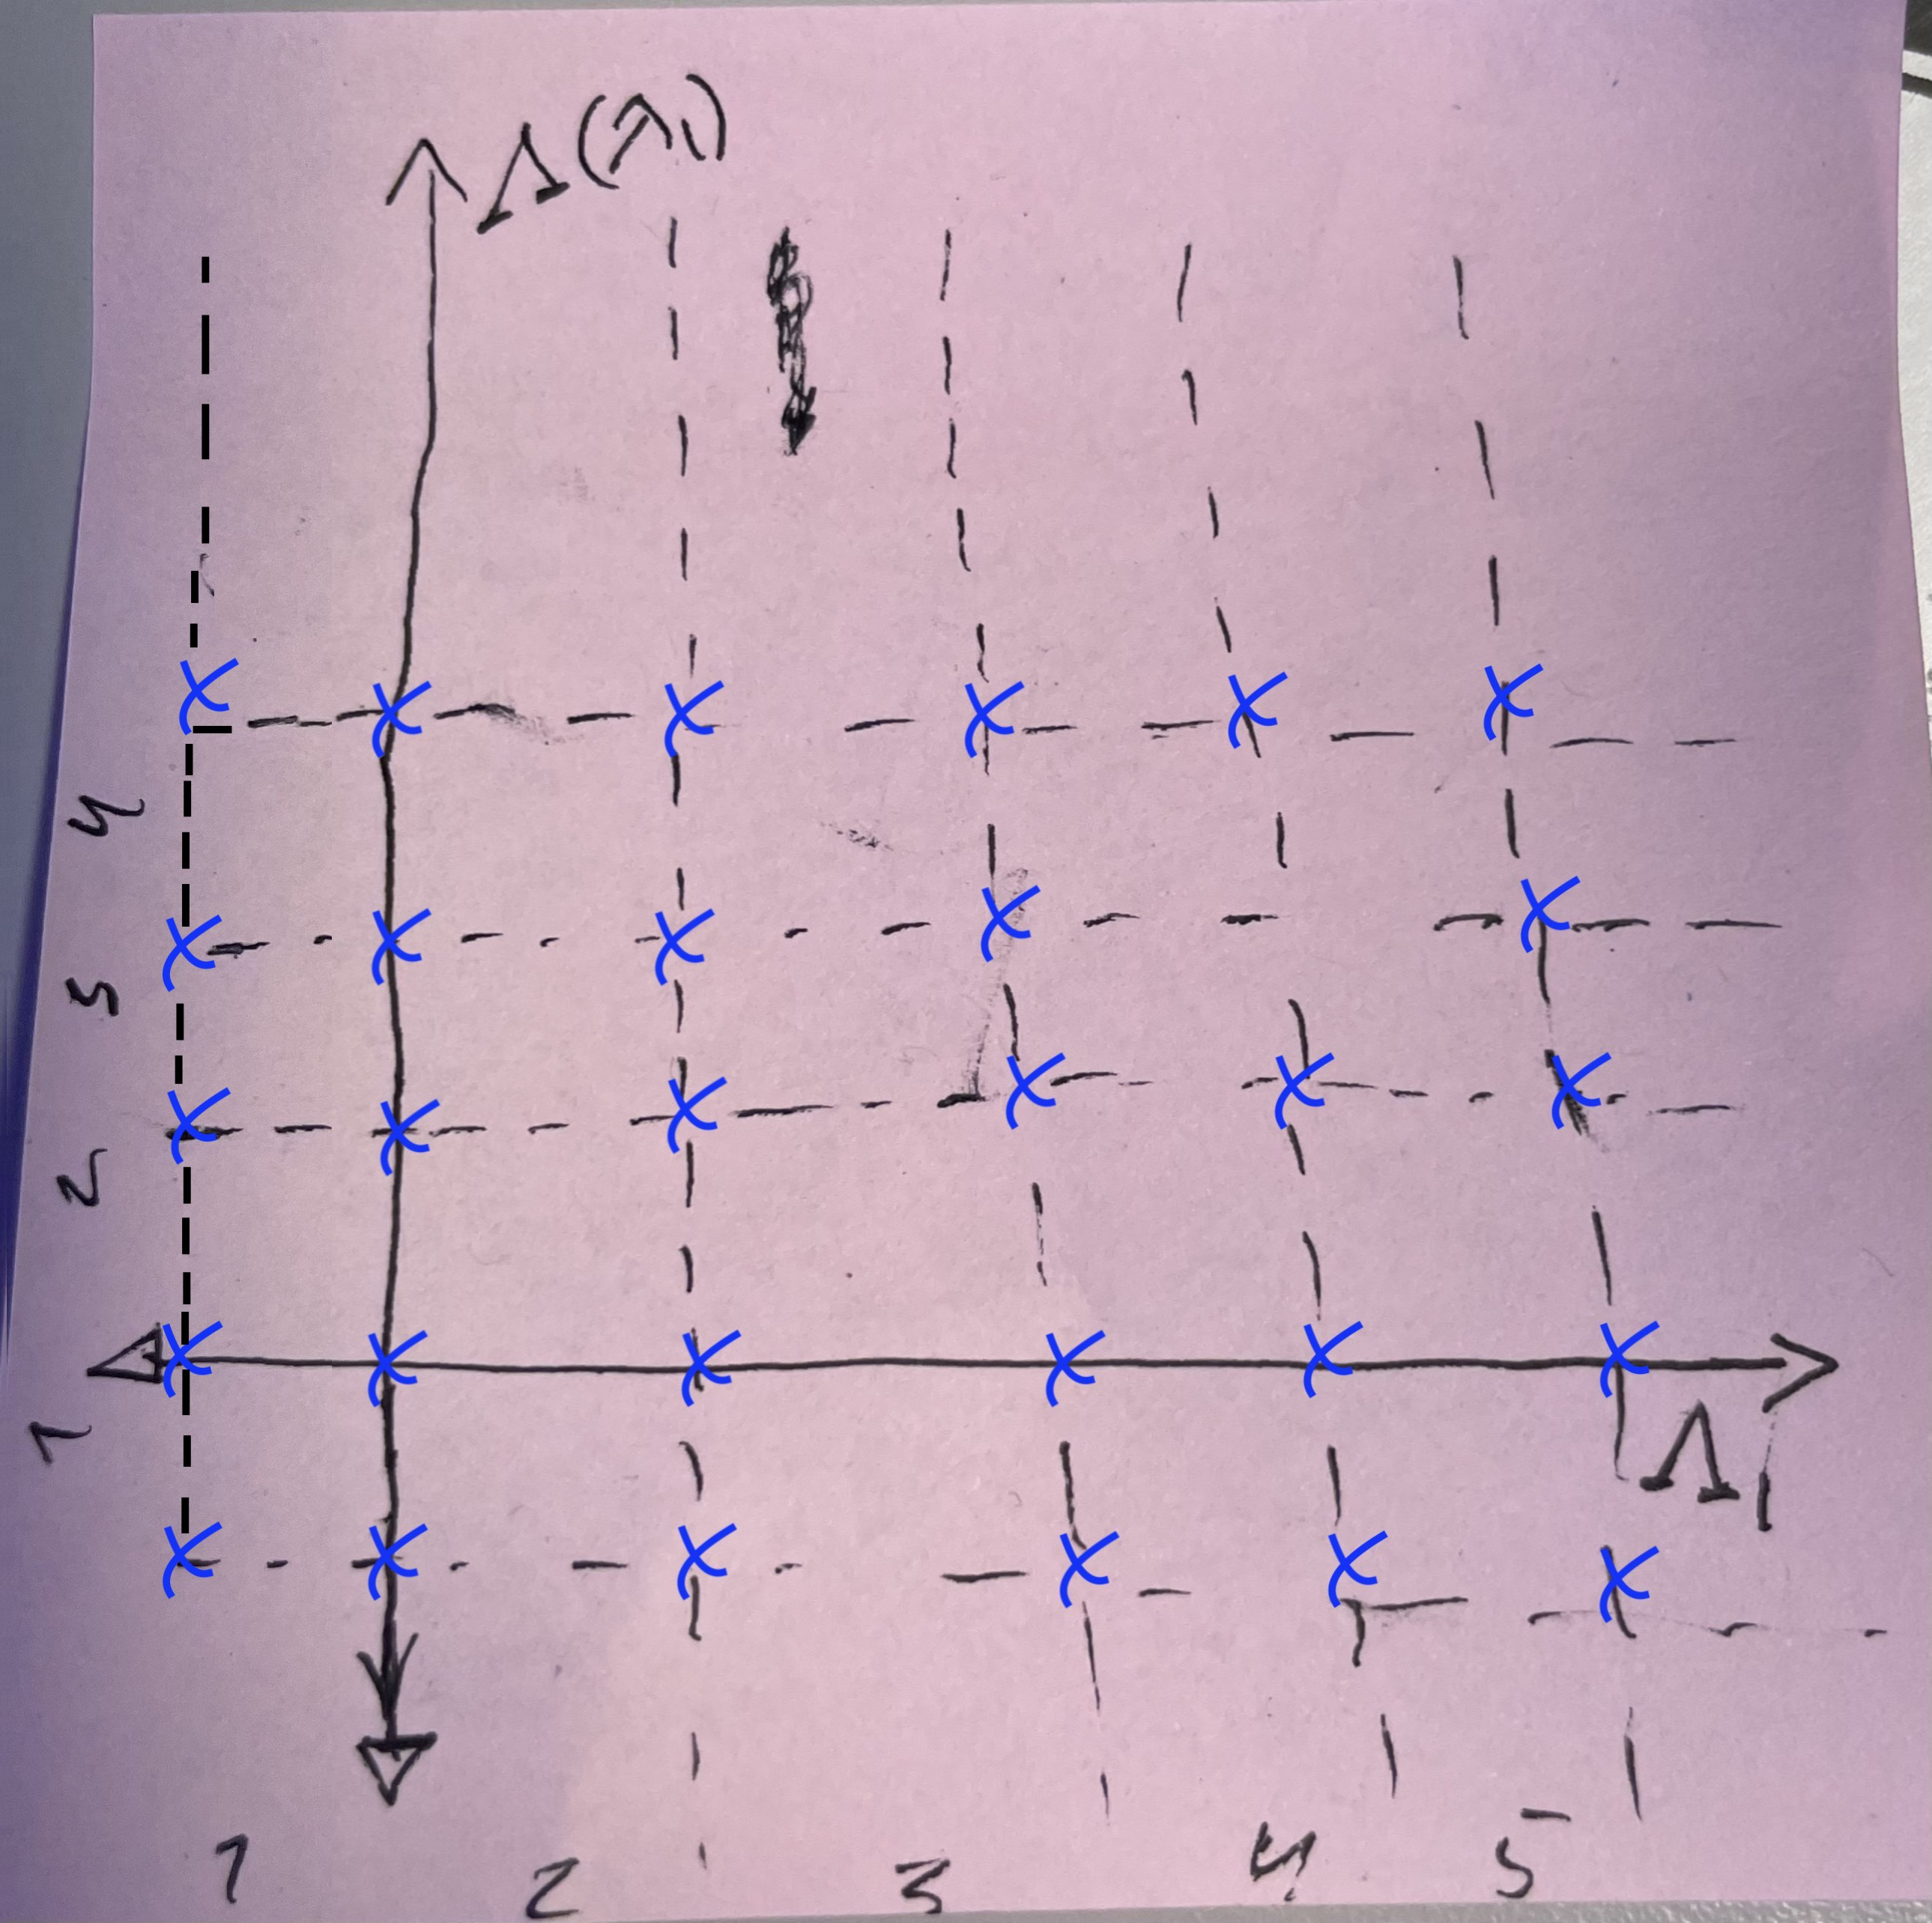
\includegraphics[width=0.9\linewidth]{spec_no_shift.jpg}
        %* Figure 1
        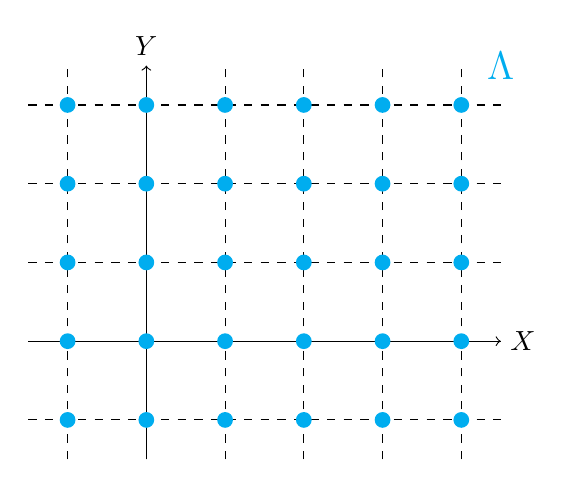
\begin{tikzpicture}
            \foreach \z in {0}{  % Controles whether the axes are inverted or not, 1 = yes, anything else = no
                

\ifnum\z=1
    % Axis lines
    %\draw[->] (-1.5,0) -- (4.5,0) node[right] {$\lambfuncGen{\lambda_2}$};
    %\draw[->] (0,-1.5) -- (0,3.5) node[above] {$\Lambda_2$};
    \draw[->] (-1.5,0) -- (4.5,0) node[right] {$Y$};
    \draw[->] (0,-1.5) -- (0,3.5) node[above] {$X$};

    % Dashed lines at each integer in the x direction
    \foreach \x in {-1,...,4}
        \draw[dashed] (\x,-1.5) -- (\x,3.5);

    % Dashed lines at each integer in the y direction
    \foreach \y in {-1,...,3}
        \draw[dashed] (-1.5,\y) -- (4.5,\y);
\else
    % Axis lines
    %\draw[->] (-1.5,0) -- (4.5,0) node[right] {$\Lambda_1$};
    %\draw[->] (0,-1.5) -- (0,3.5) node[above] {$\lambfunc$};
    \draw[->] (-1.5,0) -- (4.5,0) node[right] {$X$};
    \draw[->] (0,-1.5) -- (0,3.5) node[above] {$Y$};

    % Dashed lines at each integer in the x direction
    \foreach \x in {-1,...,4}
        \draw[dashed] (\x,-1.5) -- (\x,3.5);

    % Dashed lines at each integer in the y direction
    \foreach \y in {-1,...,3}
        \draw[dashed] (-1.5,\y) -- (4.5,\y);
\fi

% Lambda symbol in upper right corner
\node[cyan] at (4.5,3.5) {\Large $\Lambda$}; 
%\draw[orange] (4,3) node[above right] {$\Lambda$};
                % Cyan circles at an integer coordinate with no border
                \foreach \x in {-1,...,4}
                    \foreach \y in {-1,...,3}
                        \fill[cyan] (\x,\y) circle (0.1);
            }
        \end{tikzpicture}
        %* —————————————————
        \caption{Lattice spectra}
        %?  \label{fig:lattice_spectra}
    \end{subfigure}\quad
    \begin{subfigure}{.47\textwidth}
        \centering
        %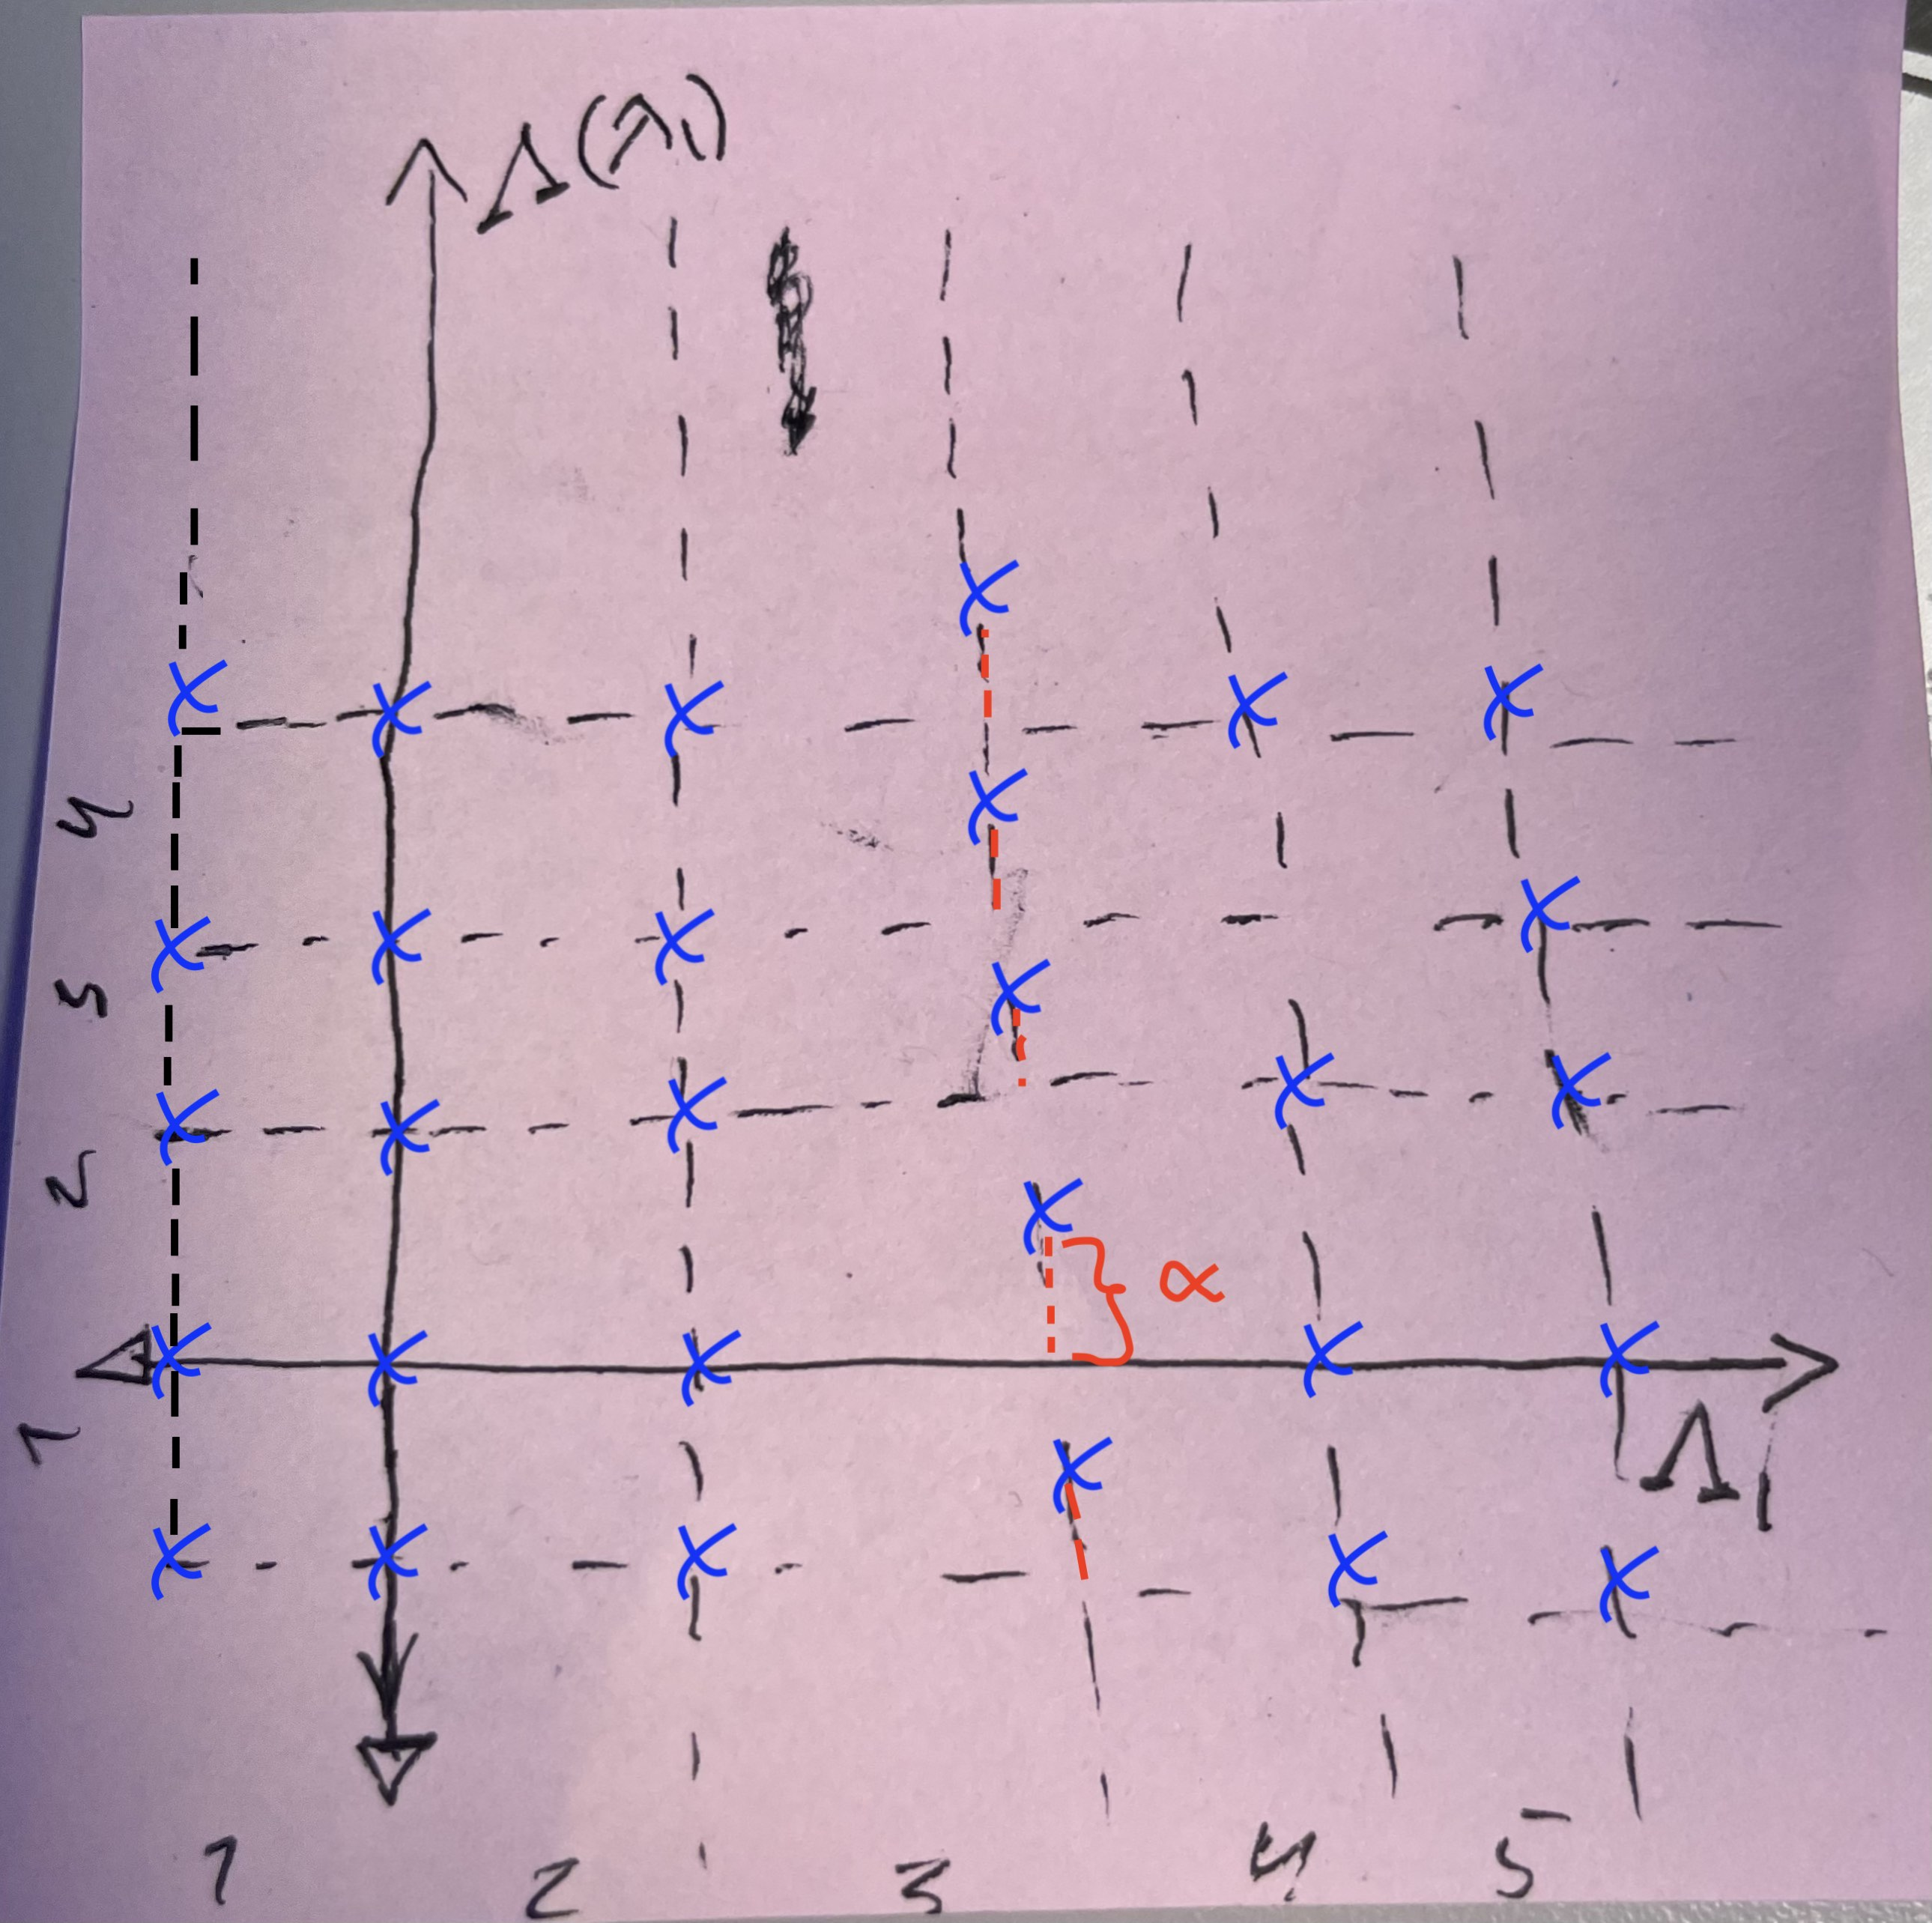
\includegraphics[width=0.9\linewidth]{spec_single_shift.jpg}
        %* Figure 2
        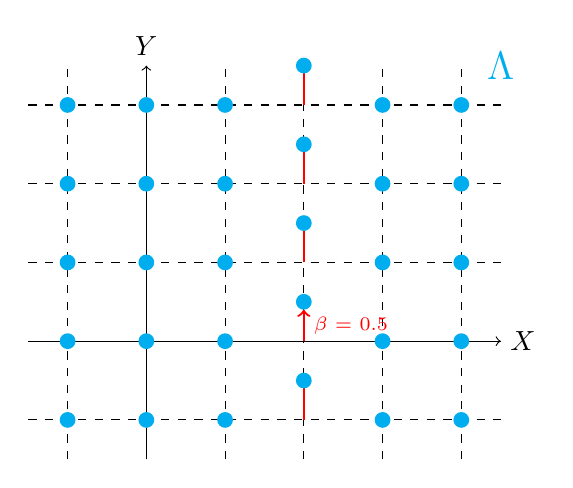
\begin{tikzpicture}
            \foreach \z in {0}{  % Controles whether the axes are inverted or not, 1 = yes, anything else = no
                

\ifnum\z=1
    % Axis lines
    %\draw[->] (-1.5,0) -- (4.5,0) node[right] {$\lambfuncGen{\lambda_2}$};
    %\draw[->] (0,-1.5) -- (0,3.5) node[above] {$\Lambda_2$};
    \draw[->] (-1.5,0) -- (4.5,0) node[right] {$Y$};
    \draw[->] (0,-1.5) -- (0,3.5) node[above] {$X$};

    % Dashed lines at each integer in the x direction
    \foreach \x in {-1,...,4}
        \draw[dashed] (\x,-1.5) -- (\x,3.5);

    % Dashed lines at each integer in the y direction
    \foreach \y in {-1,...,3}
        \draw[dashed] (-1.5,\y) -- (4.5,\y);
\else
    % Axis lines
    %\draw[->] (-1.5,0) -- (4.5,0) node[right] {$\Lambda_1$};
    %\draw[->] (0,-1.5) -- (0,3.5) node[above] {$\lambfunc$};
    \draw[->] (-1.5,0) -- (4.5,0) node[right] {$X$};
    \draw[->] (0,-1.5) -- (0,3.5) node[above] {$Y$};

    % Dashed lines at each integer in the x direction
    \foreach \x in {-1,...,4}
        \draw[dashed] (\x,-1.5) -- (\x,3.5);

    % Dashed lines at each integer in the y direction
    \foreach \y in {-1,...,3}
        \draw[dashed] (-1.5,\y) -- (4.5,\y);
\fi

% Lambda symbol in upper right corner
\node[cyan] at (4.5,3.5) {\Large $\Lambda$}; 
%\draw[orange] (4,3) node[above right] {$\Lambda$};
                % The single shift 
                \def\BetaSingle{0.5}

                % x in the range [-1,1]
                % Cyan circles at an integer coordinate with no border
                \foreach \x in {-1,...,1}
                \foreach \y in {-1,...,3}
                    \fill[cyan] (\x,\y) circle (0.1);  % Cyan circle
                    %\draw[fill=cyan] (\x,\y) circle (0.1);  % Black circle with cyan fill

                % x = 2
                \foreach \x in {2}{
                \foreach \y in {-1,...,3}{
                    \ifnum\y=0
                        \draw[->, thick, red] (\x,\y) -- (\x,\y+\BetaSingle-0.1) node[midway, right] {\scriptsize $\beta$ = \BetaSingle};  % Line indicating the shift amount
                        %\draw[thick, red] (\x,\y) -- (\x,\y+\BetaSingle-0.1) node[midway, right] {\scriptsize $\beta$ = \BetaSingle};  % Line indicating the shift amount
                    \else
                        \draw[thick, red] (\x,\y) -- (\x,\y+\BetaSingle);  % Line indicating the shift amount
                    \fi
                    \fill[cyan] (\x,\y+\BetaSingle) circle (0.1);  % Cyan circles at an integer coordinate with no border
                    %\draw[fill=cyan] (\x,\y+\BetaSingle) circle (0.1);  % Black circle with cyan fill
                }}

                % x in the range [3,4]
                % Cyan circles at an integer coordinate with no border
                \foreach \x in {3,...,4}{
                    \foreach \y in {-1,...,3}{
                        \fill[cyan] (\x,\y) circle (0.1);  % Cyan circle
                        %\draw[fill=cyan] (\x,\y) circle (0.1);  % Black circle with cyan fill
                }}
            }
        \end{tikzpicture}
        %* —————————————————
        \caption{Single shift vertical}
        %?  \label{fig:single_shift_vertical}
    \end{subfigure}\\
    \begin{subfigure}{.47\textwidth}
        \centering
        %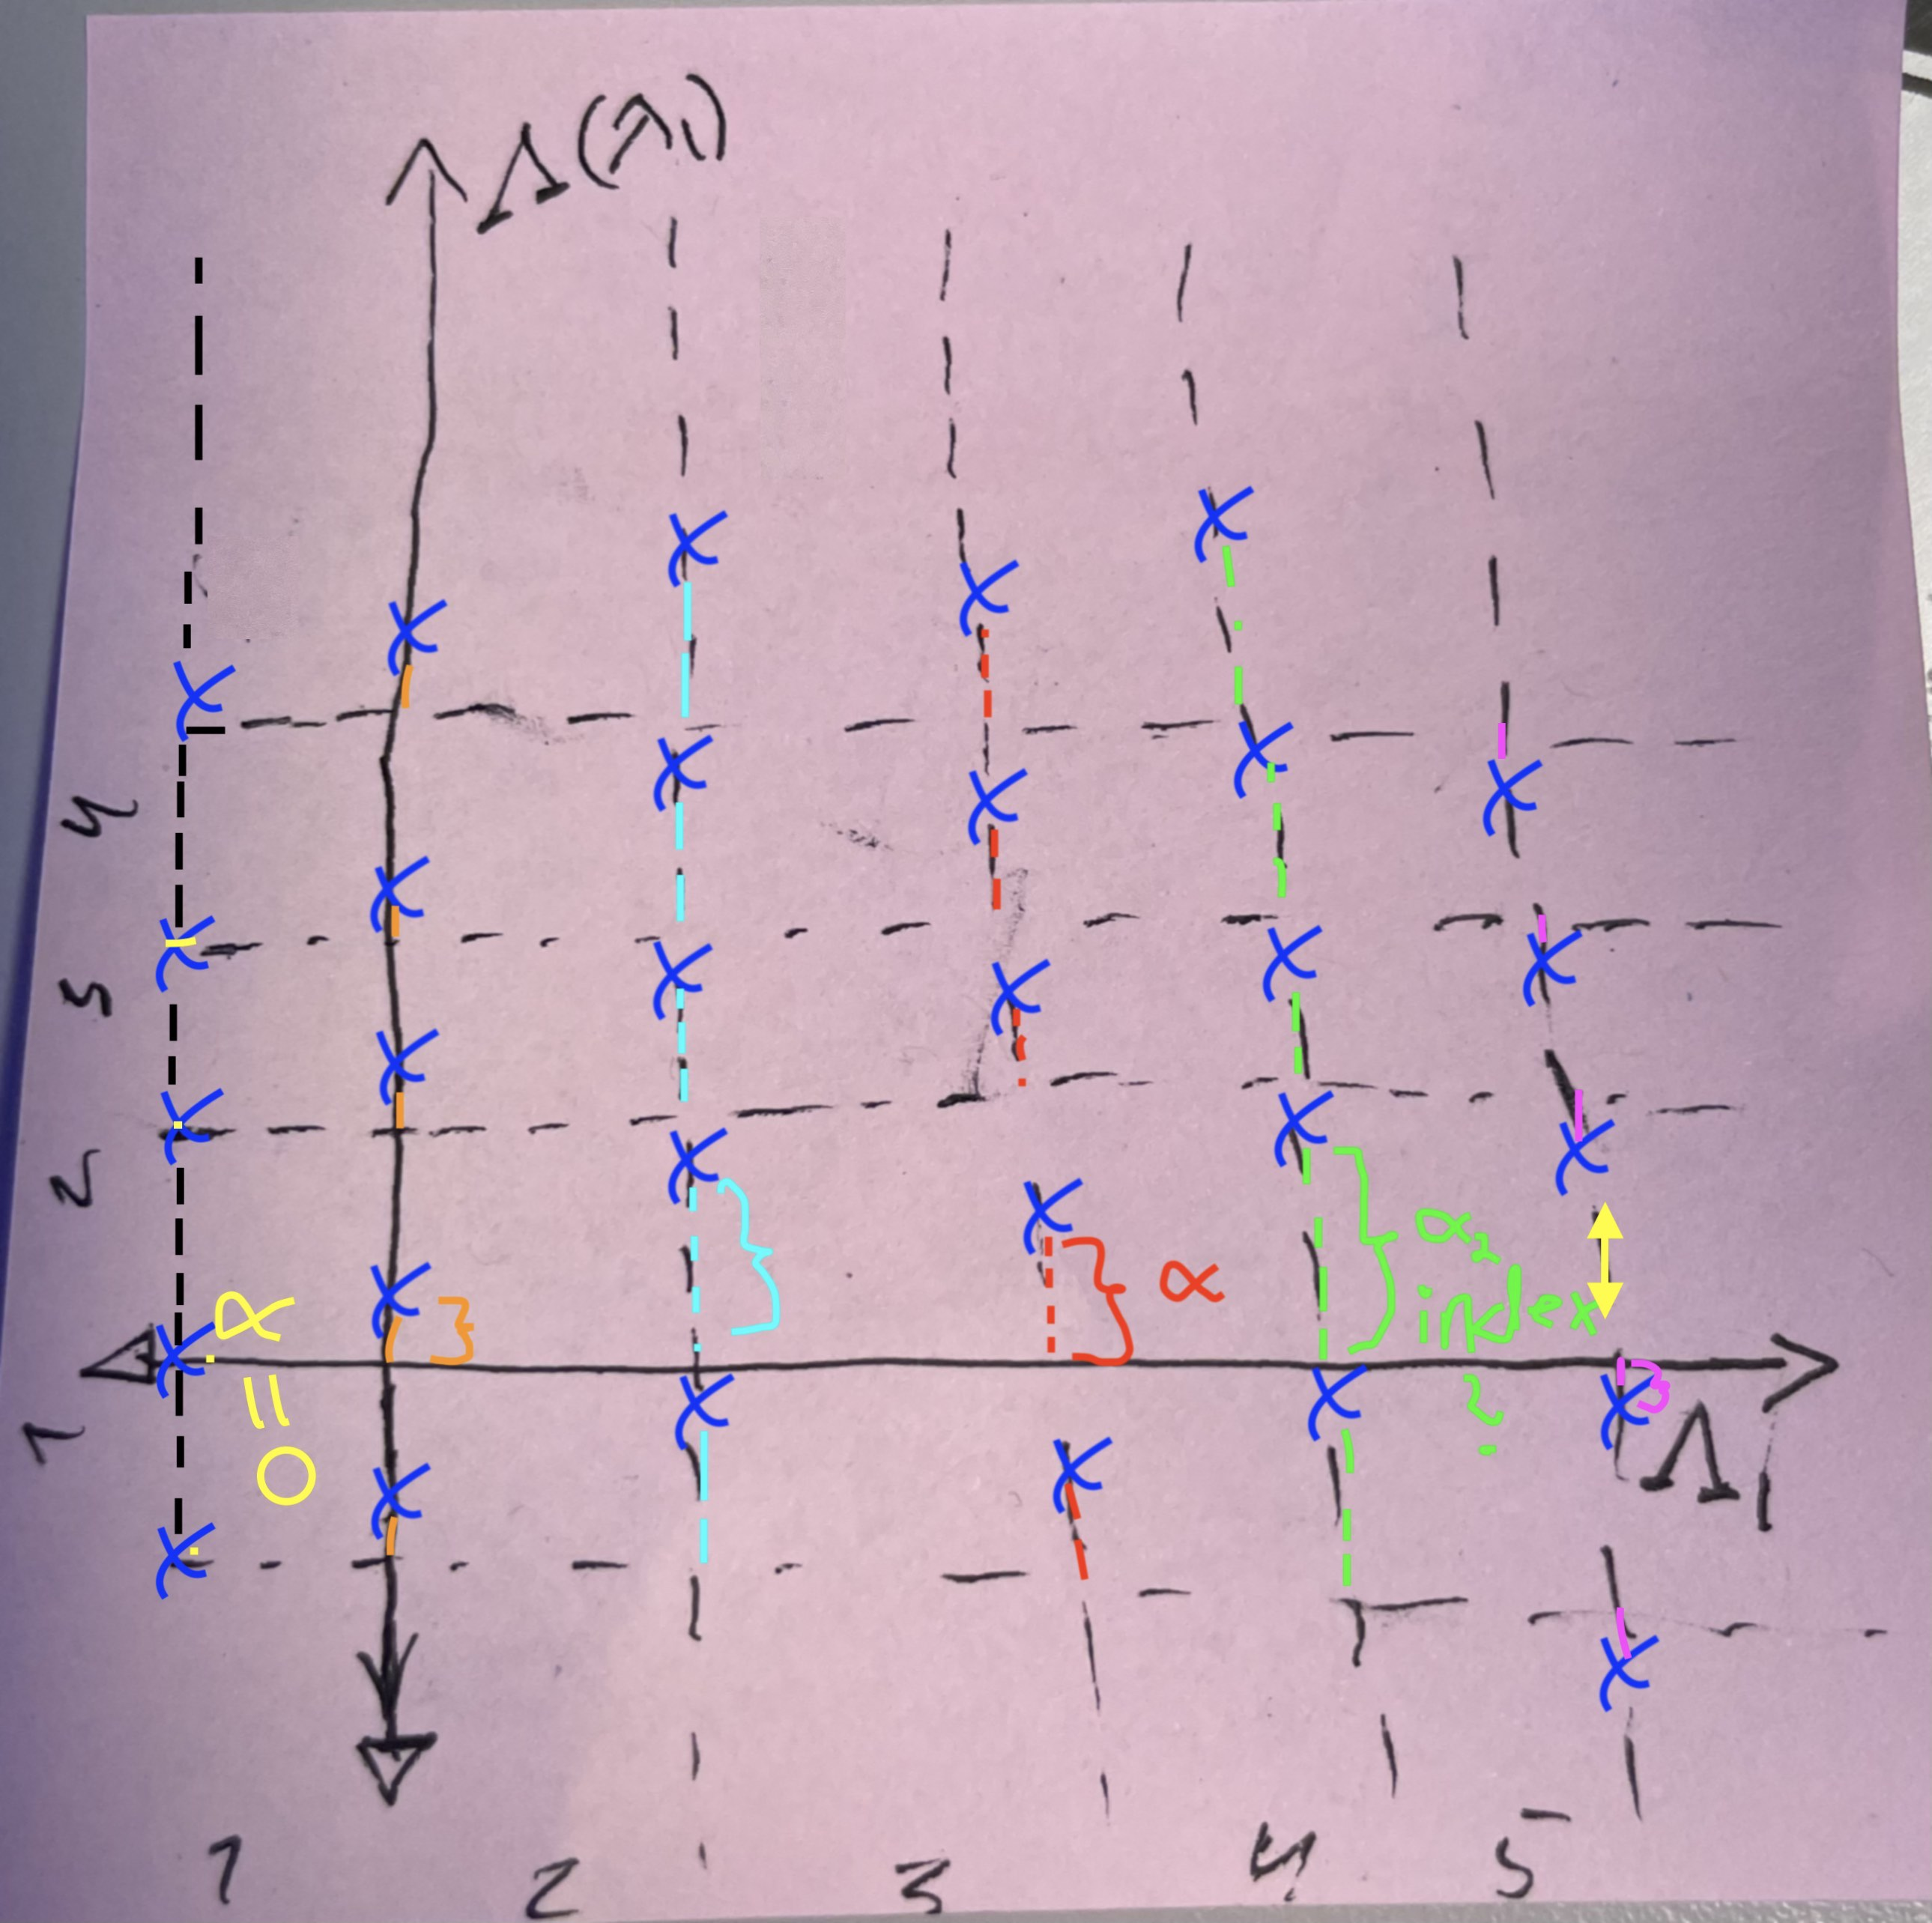
\includegraphics[width=0.9\linewidth]{multiple_shift_left_zero.jpg}
        %* Figure 3
        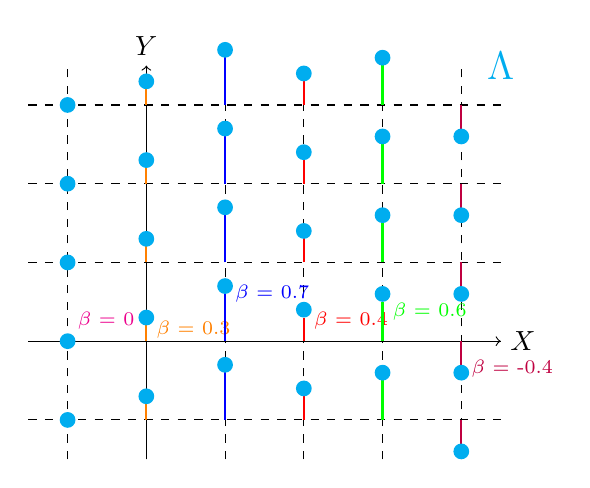
\begin{tikzpicture}
            \foreach \z in {0}{  % Controles whether the axes are inverted or not, 1 = yes, anything else = no
                

\ifnum\z=1
    % Axis lines
    %\draw[->] (-1.5,0) -- (4.5,0) node[right] {$\lambfuncGen{\lambda_2}$};
    %\draw[->] (0,-1.5) -- (0,3.5) node[above] {$\Lambda_2$};
    \draw[->] (-1.5,0) -- (4.5,0) node[right] {$Y$};
    \draw[->] (0,-1.5) -- (0,3.5) node[above] {$X$};

    % Dashed lines at each integer in the x direction
    \foreach \x in {-1,...,4}
        \draw[dashed] (\x,-1.5) -- (\x,3.5);

    % Dashed lines at each integer in the y direction
    \foreach \y in {-1,...,3}
        \draw[dashed] (-1.5,\y) -- (4.5,\y);
\else
    % Axis lines
    %\draw[->] (-1.5,0) -- (4.5,0) node[right] {$\Lambda_1$};
    %\draw[->] (0,-1.5) -- (0,3.5) node[above] {$\lambfunc$};
    \draw[->] (-1.5,0) -- (4.5,0) node[right] {$X$};
    \draw[->] (0,-1.5) -- (0,3.5) node[above] {$Y$};

    % Dashed lines at each integer in the x direction
    \foreach \x in {-1,...,4}
        \draw[dashed] (\x,-1.5) -- (\x,3.5);

    % Dashed lines at each integer in the y direction
    \foreach \y in {-1,...,3}
        \draw[dashed] (-1.5,\y) -- (4.5,\y);
\fi

% Lambda symbol in upper right corner
\node[cyan] at (4.5,3.5) {\Large $\Lambda$}; 
%\draw[orange] (4,3) node[above right] {$\Lambda$};
                % Shift list
                \def\BetaMinOne{0}
                \def\BetaZero{0.3}
                \def\BetaOne{0.7}
                \def\BetaTwo{0.4}
                \def\BetaThree{0.6}
                \def\BetaFour{-0.4}

                % x = -1
                \foreach \x in {-1}{
                \foreach \y in {-1,...,3}{
                    \ifnum\y=0
                    \draw[thick, magenta] (\x,\y) -- (\x,\y+0.05\BetaMinOne) node[midway, above right] {\scriptsize $\beta$ = \BetaMinOne};  % Line indicating the shift amount
                    \else
                    \draw[thick, magenta] (\x,\y) -- (\x,\y+\BetaMinOne);  % Line indicating the shift amount
                    \fi
                    \fill[cyan] (\x,\y+\BetaMinOne) circle (0.1);  % Cyan circles at an integer coordinate with no border
                }}
                % x = 0
                \foreach \x in {0}{
                \foreach \y in {-1,...,3}{
                    \ifnum\y=0
                    %\draw[->, orange] (\x,\y) -- (\x,\y+\BetaZero-0.1) node[near end, right] {\scriptsize $\beta$ = \BetaZero};  % Line indicating the shift amount
                    \draw[thick, orange] (\x,\y) -- (\x,\y+\BetaZero-0.1) node[near end, right] {\scriptsize $\beta$ = \BetaZero};  % Line indicating the shift amount
                    \else
                    \draw[thick, orange] (\x,\y) -- (\x,\y+\BetaZero);  % Line indicating the shift amount
                    \fi
                    \fill[cyan] (\x,\y+\BetaZero) circle (0.1);  % Cyan circles at an integer coordinate with no border
                }}
                % x = 1
                \foreach \x in {1}{
                \foreach \y in {-1,...,3}{
                    \ifnum\y=0
                    %\draw[->, blue] (\x,\y) -- (\x,\y+\BetaOne-0.1) node[at end, right] {\scriptsize $\beta$ = \BetaOne};  % Line indicating the shift amount
                    \draw[thick, blue] (\x,\y) -- (\x,\y+\BetaOne-0.1) node[at end, right] {\scriptsize $\beta$ = \BetaOne};  % Line indicating the shift amount
                    \else
                    \draw[thick, blue] (\x,\y) -- (\x,\y+\BetaOne);  % Line indicating the shift amount
                    \fi
                    \fill[cyan] (\x,\y+\BetaOne) circle (0.1);  % Cyan circles at an integer coordinate with no border
                }}
                % x = 2
                \foreach \x in {2}{
                \foreach \y in {-1,...,3}{
                    \ifnum\y=0
                    %\draw[->, red] (\x,\y) -- (\x,\y+\BetaTwo-0.1) node[very near end, right] {\scriptsize $\beta$ = \BetaTwo};  % Line indicating the shift amount
                    \draw[thick, red] (\x,\y) -- (\x,\y+\BetaTwo-0.1) node[very near end, right] {\scriptsize $\beta$ = \BetaTwo};  % Line indicating the shift amount
                    \else
                    \draw[thick, red] (\x,\y) -- (\x,\y+\BetaTwo);  % Line indicating the shift amount
                    \fi
                    \fill[cyan] (\x,\y+\BetaTwo) circle (0.1);  % Cyan circles at an integer coordinate with no border
                }}
                % x = 3
                \foreach \x in {3}{
                \foreach \y in {-1,...,3}{
                    \ifnum\y=0
                    %\draw[->, green] (\x,\y) -- (\x,\y+\BetaThree-0.1) node[near end, right] {\scriptsize $\beta$ = \BetaThree};  % Line indicating the shift amount
                    \draw[thick, green] (\x,\y) -- (\x,\y+\BetaThree-0.1) node[near end, right] {\scriptsize $\beta$ = \BetaThree};  % Line indicating the shift amount
                    \else
                    \draw[thick, green] (\x,\y) -- (\x,\y+\BetaThree);  % Line indicating the shift amount
                    \fi
                    \fill[cyan] (\x,\y+\BetaThree) circle (0.1);  % Cyan circles at an integer coordinate with no border
                }}
                % x = 4
                \foreach \x in {4}{
                \foreach \y in {-1,...,3}{
                    \ifnum\y=0
                    %\draw[->, purple] (\x,\y) -- (\x,\y+\BetaFour+0.1) node[at end, right, yshift=-0.5mm] {\scriptsize $\beta$ = \BetaFour};  % Line indicating the shift amount
                    \draw[thick, purple] (\x,\y) -- (\x,\y+\BetaFour+0.1) node[at end, right, yshift=-0.5mm] {\scriptsize $\beta$ = \BetaFour};  % Line indicating the shift amount
                    \else
                    \draw[thick, purple] (\x,\y) -- (\x,\y+\BetaFour);  % Line indicating the shift amount
                    \fi
                    \fill[cyan] (\x,\y+\BetaFour) circle (0.1);  % Cyan circles at an integer coordinate with no border
                }}
            }
        \end{tikzpicture}
        %* —————————————————
        \caption{Multiple individual shifts vertical}
        %?  \label{fig:multiple_shift_vertical}
    \end{subfigure}\quad
    \begin{subfigure}{.47\textwidth}
        \centering
        %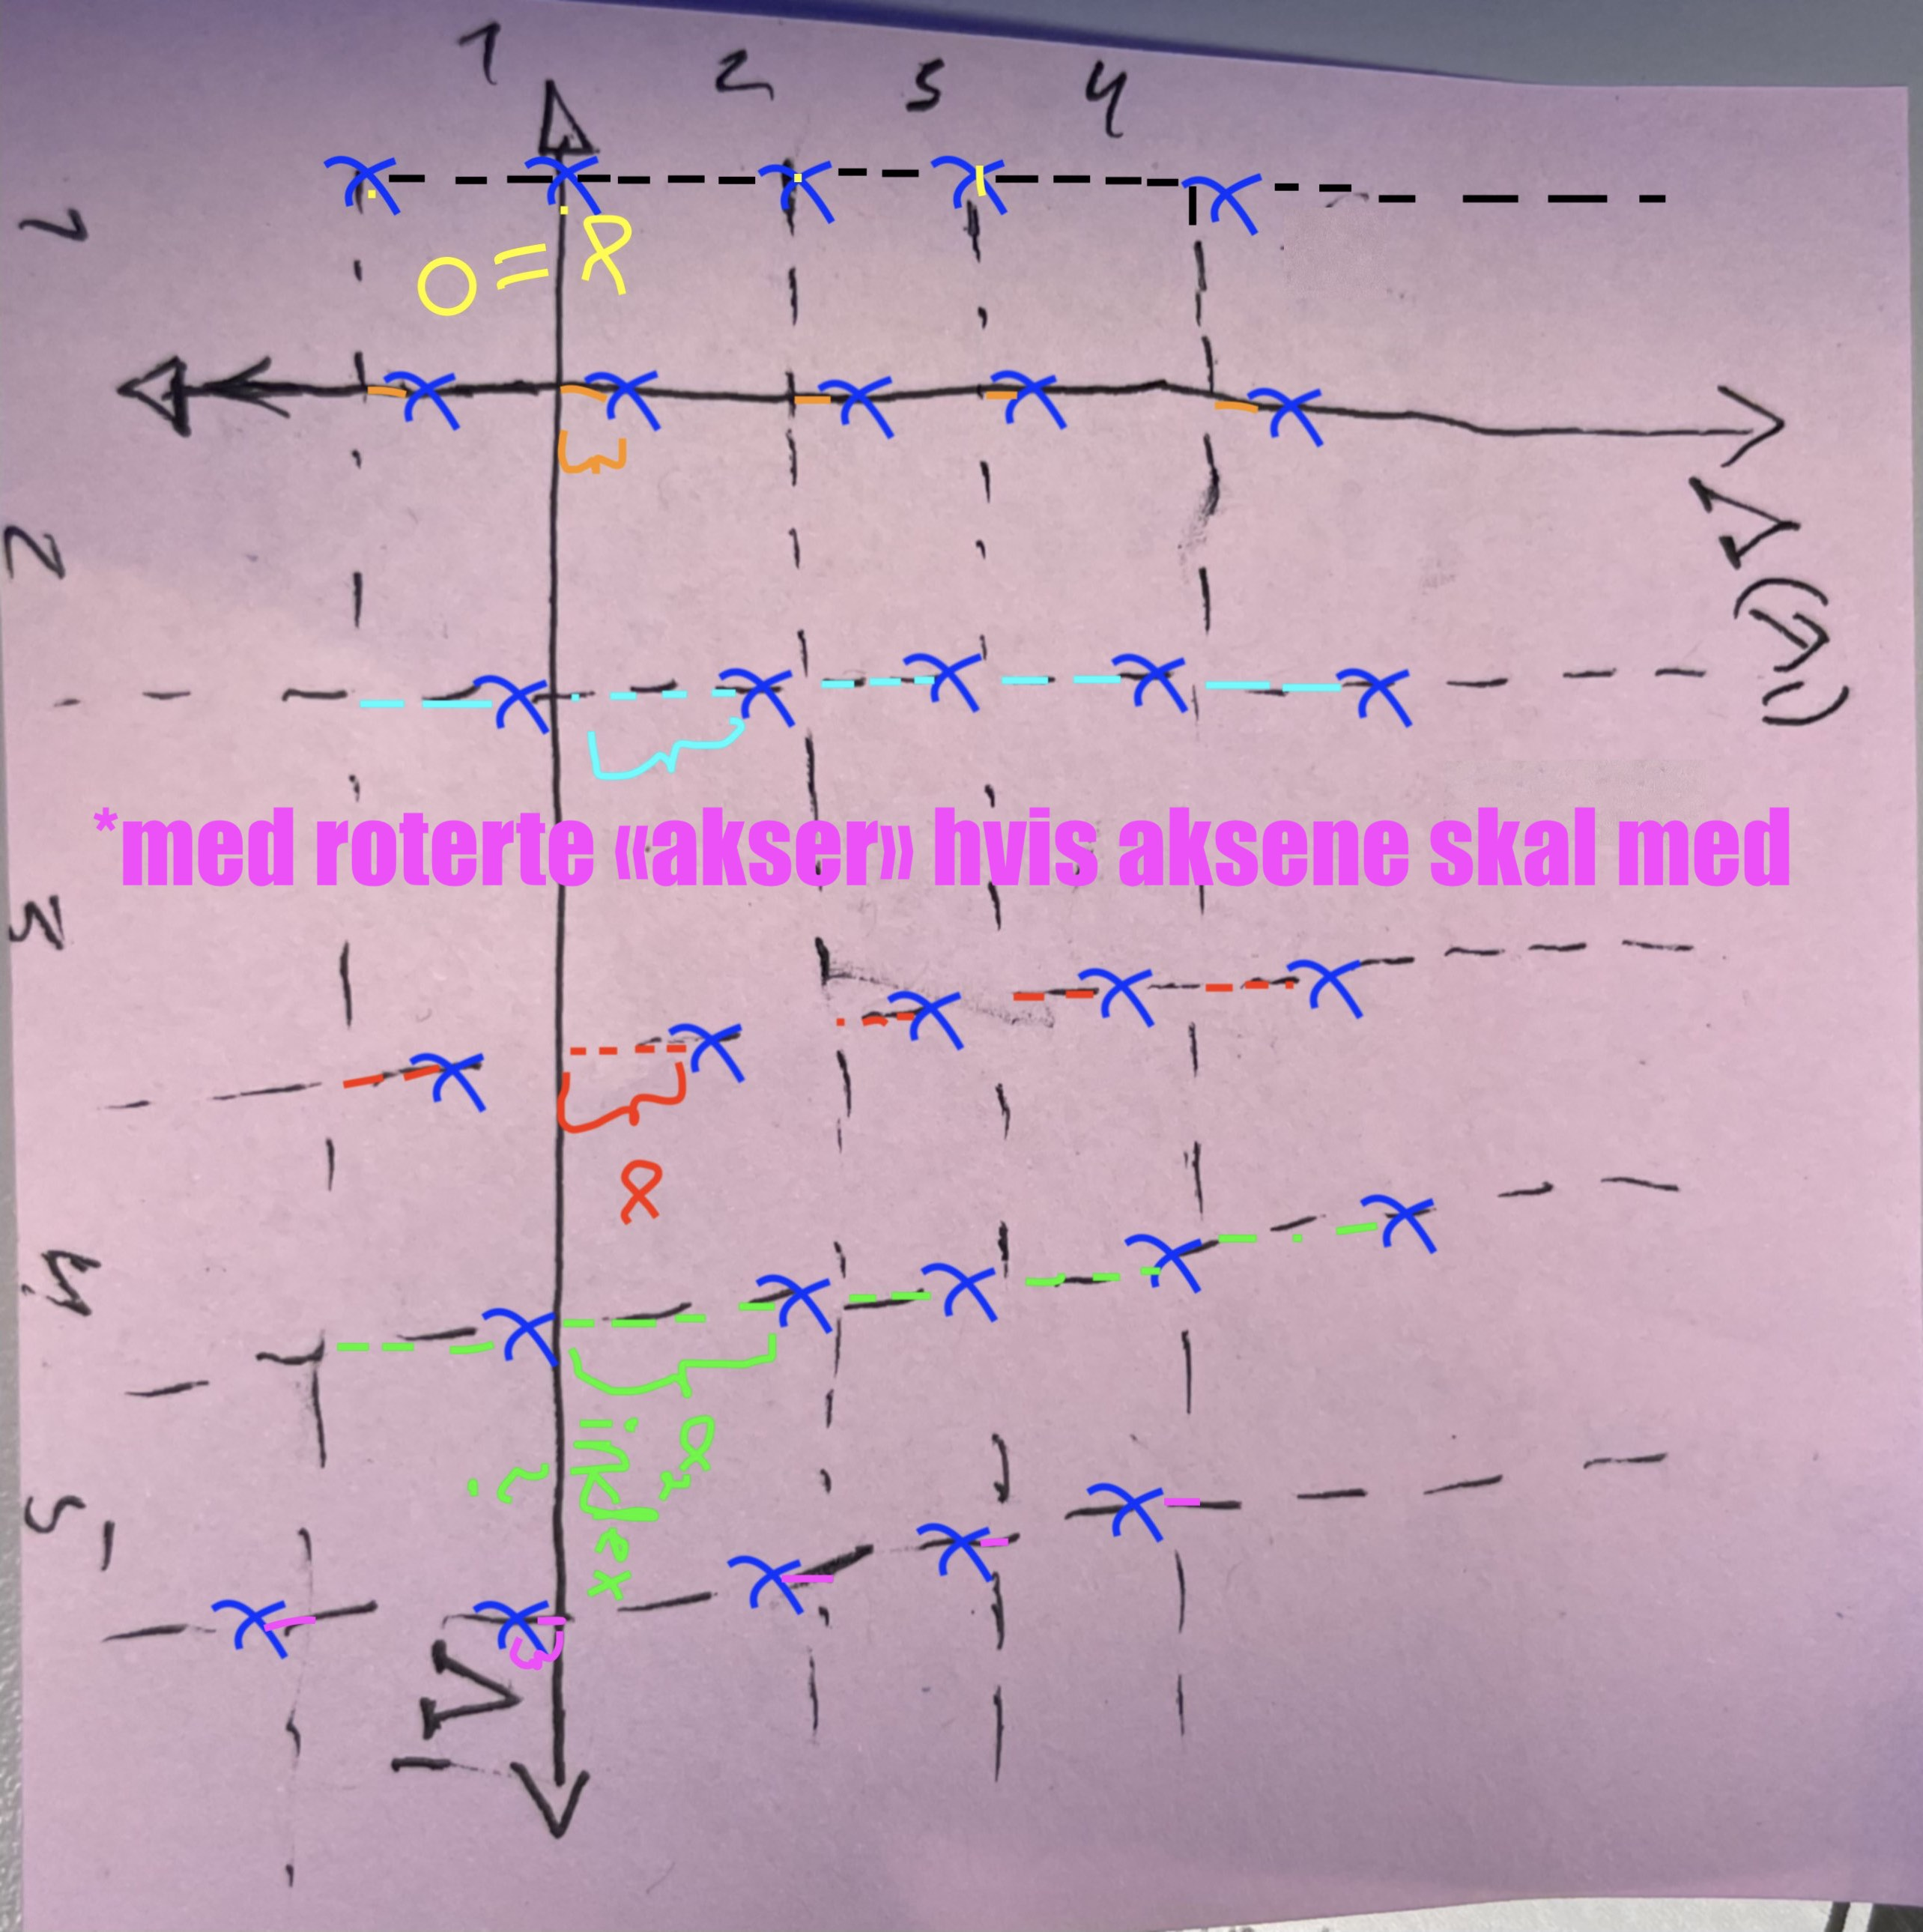
\includegraphics[width=0.9\linewidth]{multiple_shift_left_zero_horizontal.jpg}
        %* Figure 4
        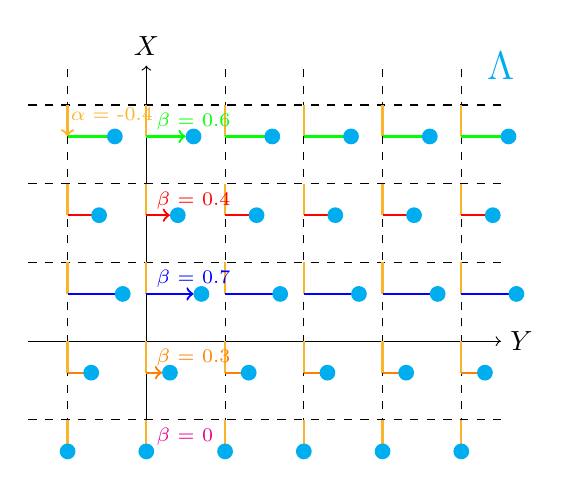
\begin{tikzpicture}
            \foreach \z in {1}{  % Controles whether the axes are inverted or not, 1 = yes, anything else = no
                

\ifnum\z=1
    % Axis lines
    %\draw[->] (-1.5,0) -- (4.5,0) node[right] {$\lambfuncGen{\lambda_2}$};
    %\draw[->] (0,-1.5) -- (0,3.5) node[above] {$\Lambda_2$};
    \draw[->] (-1.5,0) -- (4.5,0) node[right] {$Y$};
    \draw[->] (0,-1.5) -- (0,3.5) node[above] {$X$};

    % Dashed lines at each integer in the x direction
    \foreach \x in {-1,...,4}
        \draw[dashed] (\x,-1.5) -- (\x,3.5);

    % Dashed lines at each integer in the y direction
    \foreach \y in {-1,...,3}
        \draw[dashed] (-1.5,\y) -- (4.5,\y);
\else
    % Axis lines
    %\draw[->] (-1.5,0) -- (4.5,0) node[right] {$\Lambda_1$};
    %\draw[->] (0,-1.5) -- (0,3.5) node[above] {$\lambfunc$};
    \draw[->] (-1.5,0) -- (4.5,0) node[right] {$X$};
    \draw[->] (0,-1.5) -- (0,3.5) node[above] {$Y$};

    % Dashed lines at each integer in the x direction
    \foreach \x in {-1,...,4}
        \draw[dashed] (\x,-1.5) -- (\x,3.5);

    % Dashed lines at each integer in the y direction
    \foreach \y in {-1,...,3}
        \draw[dashed] (-1.5,\y) -- (4.5,\y);
\fi

% Lambda symbol in upper right corner
\node[cyan] at (4.5,3.5) {\Large $\Lambda$}; 
%\draw[orange] (4,3) node[above right] {$\Lambda$};
                % Shift list
                \def\BetaMinOne{0}
                \def\BetaZero{0.3}
                \def\BetaOne{0.7}
                \def\BetaTwo{0.4}
                \def\BetaThree{0.6}
                \def\BetaFour{-0.6}
                \def\AlphaONE{-0.4}

                % The X shift lines at x=0
                \foreach \x in {-1,...,4}{
                \foreach \y in {-1,...,3}{
                    \ifnum\x=-1
                        \ifnum\y=3
                            \draw[->, thick, Dandelion] (\x,\y) -- (\x,\y+\AlphaONE) node[pos=0.3, right, xshift=-0.9mm] {\scriptsize $\alpha$ = \AlphaONE};  % Line indicating the shift amount
                        \else
                            %\draw[->, thick, purple] (\x,\y) -- (\x,\y+\AlphaONE);  % Line indicating the shift amount
                            \draw[thick, Dandelion] (\x,\y) -- (\x,\y+\AlphaONE);  % Line indicating the shift amount
                        \fi
                    \else
                    \draw[thick, Dandelion] (\x,\y) -- (\x,\y+\AlphaONE);  % Line indicating the shift amount
                    \fi
                }}

                % The Y shift
                % y = -1
                \foreach \y in {-1}{
                \foreach \x in {-1,...,4}{
                    \ifnum\x=0
                    % no arrow here. It looks ugly for thick lines
                    \draw[thick, magenta] (\x,\y+\AlphaONE) -- (\x+\BetaMinOne+0.05, \y+\AlphaONE) node[at start, above right, yshift=-0.5mm] {\scriptsize $\beta$ = \BetaMinOne};  % Line indicating the shift amount
                    \else
                    \draw[thick, magenta] (\x,\y+\AlphaONE) -- (\x+\BetaMinOne,\y+\AlphaONE);  % Line indicating the shift amount
                    \fi
                    \fill[cyan] (\x+\BetaMinOne,\y+\AlphaONE) circle (0.1);  % Cyan circles at an integer coordinate with no border
                }}
                % y = 0
                \foreach \y in {0}{
                \foreach \x in {-1,...,4}{
                    \ifnum\x=0
                    \draw[->, thick, orange] (\x,\y+\AlphaONE) -- (\x+\BetaZero-0.1,\y+\AlphaONE) node[at start, above right, yshift=-0.5mm] {\scriptsize $\beta$ = \BetaZero};  % Line indicating the shift amount
                    \else
                    \draw[thick, orange] (\x,\y+\AlphaONE) -- (\x+\BetaZero,\y+\AlphaONE);  % Line indicating the shift amount
                    \fi
                    \fill[cyan] (\x+\BetaZero,\y+\AlphaONE) circle (0.1);  % Cyan circles at an integer coordinate with no border
                }}
                % y = 1
                \foreach \y in {1}{
                \foreach \x in {-1,...,4}{
                    \ifnum\x=0
                    \draw[->, thick, blue] (\x,\y+\AlphaONE) -- (\x+\BetaOne-0.1,\y+\AlphaONE) node[at start, above right, yshift=-0.5mm] {\scriptsize $\beta$ = \BetaOne};  % Line indicating the shift amount
                    \else
                    \draw[thick, blue] (\x,\y+\AlphaONE) -- (\x+\BetaOne,\y+\AlphaONE);  % Line indicating the shift amount
                    \fi
                    \fill[cyan] (\x+\BetaOne,\y+\AlphaONE) circle (0.1);  % Cyan circles at an integer coordinate with no border
                }}
                % y = 2
                \foreach \y in {2}{
                \foreach \x in {-1,...,4}{
                    \ifnum\x=0
                    \draw[->, thick, red] (\x,\y+\AlphaONE) -- (\x+\BetaTwo-0.1,\y+\AlphaONE) node[at start, above right, yshift=-0.5mm] {\scriptsize $\beta$ = \BetaTwo};  % Line indicating the shift amount
                    \else
                    \draw[thick, red] (\x,\y+\AlphaONE) -- (\x+\BetaTwo,\y+\AlphaONE);  % Line indicating the shift amount
                    \fi
                    \fill[cyan] (\x+\BetaTwo,\y+\AlphaONE) circle (0.1);  % Cyan circles at an integer coordinate with no border
                }}
                % y = 3
                \foreach \y in {3}{
                \foreach \x in {-1,...,4}{
                    \ifnum\x=0
                    \draw[->, thick, green] (\x,\y+\AlphaONE) -- (\x+\BetaThree-0.1,\y+\AlphaONE) node[at start, above right, yshift=-0.5mm] {\scriptsize $\beta$ = \BetaThree};  % Line indicating the shift amount
                    \else
                    \draw[thick, green] (\x,\y+\AlphaONE) -- (\x+\BetaThree,\y+\AlphaONE);  % Line indicating the shift amount
                    \fi
                    \fill[cyan] (\x+\BetaThree,\y+\AlphaONE) circle (0.1);  % Cyan circles at an integer coordinate with no border
                }}
            }
        \end{tikzpicture}
        %* —————————————————
        \caption{Multiple individual shifts horizontal}
        %?  \label{fig:multiple_shift_horizontal}
    \end{subfigure}
    %?  \label{fig:spectra_figures}
    % \caption{Illustration of four spectral pairs for $(I^2,\Lambda)$ on a coordinate plane $X\times Y$. Dashed lines highlight the coordinate plane itself, and the cyan circles represent elements from the spectrum. In \cref{fig:lattice_spectra,fig:single_shift_vertical} $\Lambda$ is given by \labelcref{eq:first_construction} and \labelcref{eq:lam_single_shift_vertical} respectivly, where $\beta=0.5$ for the latter. In \cref{fig:multiple_shift_vertical,fig:multiple_shift_horizontal} $\Lambda$ is given by \labelcref{eq:lam_multiple_shift_vertical,eq:lam_multiple_shift_horizontal} respectivly.}
\end{figure}

}  %! End

\clearpage
The author's thesis structure. No need to copy this "organized mess". Note the pinned \verb|thesis.tex| and \verb|commands.tex|, and also the happy pets down below. 
\begin{figure}[h!]
    \centering
    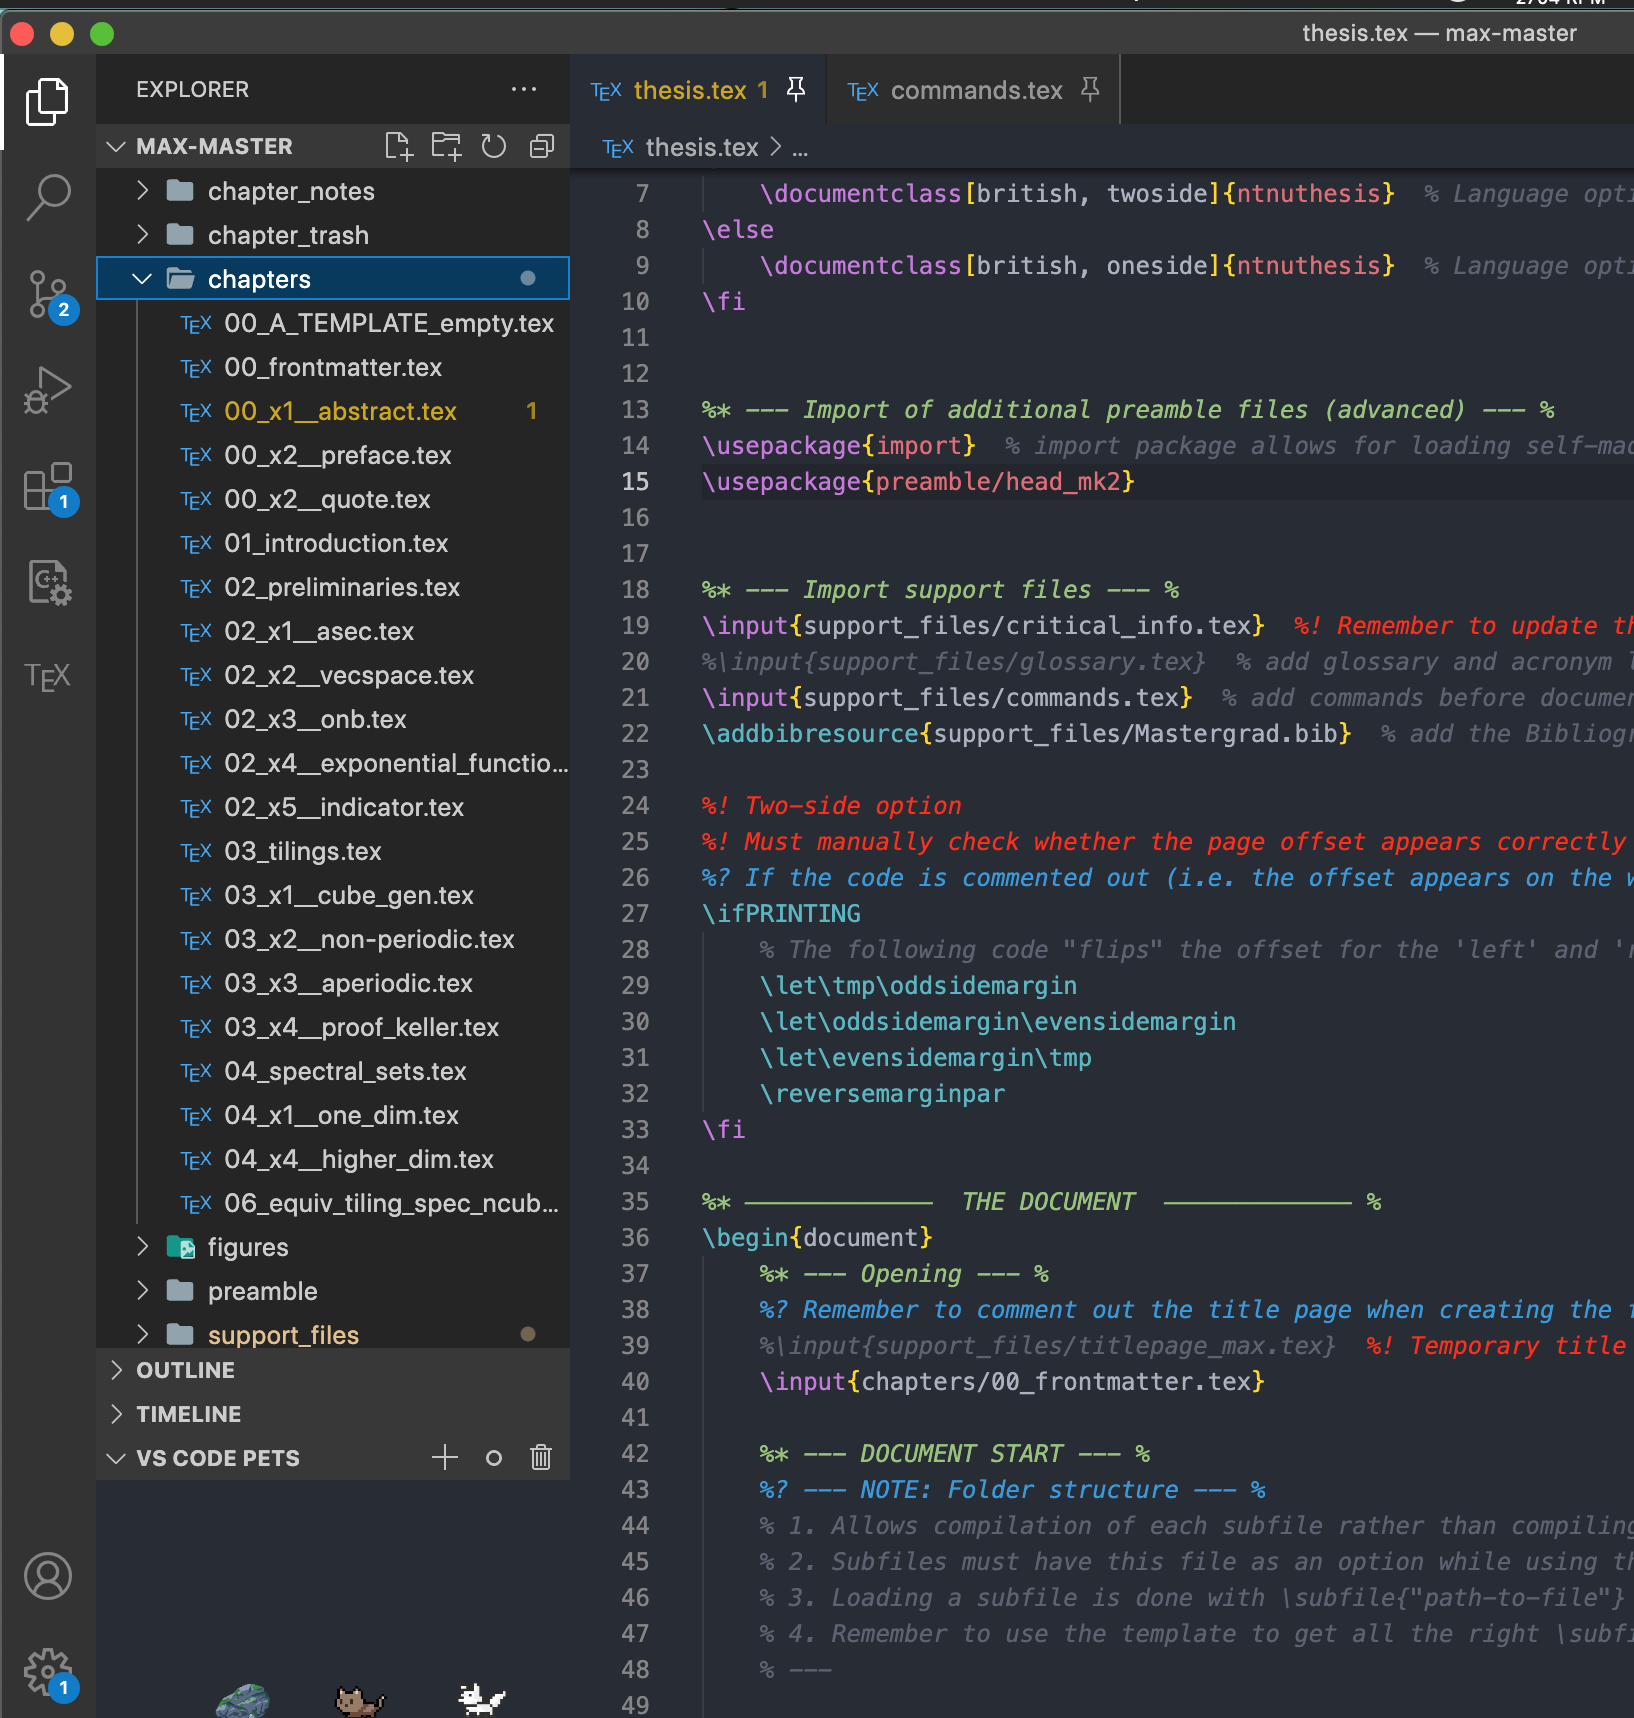
\includegraphics[width=0.8\linewidth]{one_ex.png}
\end{figure}


\end{document}


